% --------------------------------------------------------------
% This is all preamble stuff that you don't have to worry about.
% Head down to where it says "Start here"
% --------------------------------------------------------------

\documentclass[12pt]{report}

\usepackage{graphicx}
\usepackage[margin=1in]{geometry}
\usepackage{amsmath,amsthm,amssymb, diagbox, enumerate, textcomp, caption, subcaption, tabu, xcolor, csquotes,tcolorbox}
\usepackage{tikz}
\usetikzlibrary{mindmap}
\usepackage{hyperref}
\usepackage{float}
\usepackage{pgfplots}
\usepackage{tikz-cd}
\usepackage{mathtools}
\pgfplotsset{compat=1.15}

\newtcolorbox{mybox}{fontupper=\footnotesize}


\usepackage[export]{adjustbox}% 'export' allows adjustbox keys in \includegraphics



\usepackage{chngcntr}

\counterwithin*{equation}{section}
\counterwithin*{equation}{subsection}

\usepackage[style=authoryear]{biblatex}
\addbibresource{references.bib}% Syntax for version >= 1.2

% English language.
\usepackage[english]{babel}


\usepackage[notextcomp]{stix}% Stix font
\usepackage{helvet}% Helvetica, served as a model for arial
\usepackage{xcolor}
\usepackage{titlesec}
\titleformat{\chapter}[display]
  {\normalfont\sffamily\huge\bfseries}
  {\chaptertitlename\ \thechapter}{20pt}{\Huge}
\titleformat{\section}
  {\normalfont\sffamily\Large\bfseries}
  {\thesection}{1em}{}
  \titleformat{\subsection}
  {\normalfont\sffamily\large\bfseries}
  {\thesubsection}{1em}{}
   \titleformat{\subsubsection}
  {\normalfont\sffamily\normalsize\bfseries}
  {\thesubsubsection}{1em}{}
     \titleformat{\paragraph}
  {\normalfont\sffamily\normalsize\bfseries}
  {\theparagraph}{1em}{}


\definecolor{gray75}{gray}{0.75}
\newcommand{\hsp}{\hspace{20pt}}
\titleformat{\chapter}[hang]{\Huge\normalfont\sffamily\bfseries}{\thechapter\hsp\textcolor{gray75}{|}\hsp}{0pt}{\Huge\normalfont\sffamily\bfseries}

\usepackage[T1]{fontenc}
\usepackage{titlesec, blindtext, color}
\definecolor{gray75}{gray}{0.75}
%\newcommand{\hsp}{\hspace{20pt}}
\titleformat{\chapter}[hang]{\sffamily\Huge\bfseries}{\thechapter\hsp\textcolor{gray75}{|}\hsp}{0pt}{\sffamily\Huge\bfseries}






\newenvironment{theorem}[2][Theorem]{\begin{trivlist}
\item[\hskip \labelsep {\bfseries #1}\hskip \labelsep {\bfseries #2.}]}{\end{trivlist}}
\newenvironment{lemma}[2][Lemma]{\begin{trivlist}
\item[\hskip \labelsep {\bfseries #1}\hskip \labelsep {\bfseries #2.}]}{\end{trivlist}}
\newenvironment{exercise}[2][Exercise]{\begin{trivlist}
\item[\hskip \labelsep {\bfseries #1}\hskip \labelsep {\bfseries #2.}]}{\end{trivlist}}
\newenvironment{reflection}[2][Reflection]{\begin{trivlist}
\item[\hskip \labelsep {\bfseries #1}\hskip \labelsep {\bfseries #2.}]}{\end{trivlist}}



\begin{document}

% --------------------------------------------------------------
%                         Start here
% --------------------------------------------------------------

%\renewcommand{\qedsymbol}{\filledbox}

\title{
Lecture Notes \\
\large Macroeconomics \\
MeC @ ISEG --- 2018/2019
}
\author{Olaf Ghanizadeh}




\maketitle


\tableofcontents

\newpage

\chapter{Economic Growth Theory}
\section{Trend and business cycle: long-run stylised facts}

\section{The Solow-Swan model}\label{solow-swan-model}
\subsection*{General assumptions}
\begin{enumerate}
    \item A closed economy
    \item No Government, thus we do not have to consider taxes and all income is available for consumption
\end{enumerate}

\textbf{Assumes a Neoclassical production function:}
\begin{equation}\label{production_function}
Y(t)=F\left[B(t)K(t), A(t)L(t)\right]
\end{equation}
 where
 \begin{align*}
 \frac{\partial F}{\partial (B,K)}>0
 &&
 \frac{\partial F}{\partial (A,L)}>0
 \end{align*}

We are familiar with this production function and its inputs. $B$ and $A$ represent effectiveness of capital and labor respectively. 

The production function \ref{production_function} has a few mathematical characteristics:
\begin{itemize}
\item
  It is a positive function, i.e.~the output cannot be negative
\item
  To simplify we assume that the function is continuous and
  twice-differentiable
\item
  Marginal productivity is positive
\item
  Returns to scale are constant
  \begin{itemize}
  \item The economy is big enough to have exhausted the gains from specialization
  \item In a small economy we can expect "more than double" increase in output with specialization (Economies of Scale i.e.)
  \end{itemize}
  \item Inputs other than capital, labour and knowledge are not important, such as land other natural resources. 
\item
  The model satisfies the Inada-conditions
 
\begin{align*}
\lim_{B * K \rightarrow 0 } \frac{\partial F}{\partial (B,K)}= \infty   
&&
\lim_{A * L \rightarrow 0 } \frac{\partial F}{\partial (A,L)}= \infty
\end{align*}

\begin{align*}
\lim_{B * K \rightarrow \infty } \frac{\partial F}{\partial (B,K)}= 0    
&&
\lim_{A * L \rightarrow \infty } \frac{\partial F}{\partial (A,L)}= 0
\end{align*}

  \begin{itemize}
  \item
    In economic terms it says that marginal product of capital is very large when the capital stock is sufficiently small and that it becomes smaller when capital grows. Imagine an economy with $K(0)$; it will not have any output. When we introduce a little bit of capital, the marginal product of that initial capital is very high. 
  \end{itemize}
\end{itemize}

\subsubsection*{Production Functions with different forms of technical progress}
The model can use technical progress, we have have a few different types of technical progress. It is useful to notice that such progress can be both tangible and intangible. An example is how the increased hand-hygiene in hospitals significantly reduced the amount of hospital related deaths. 

\subsubsection*{Capital Augmenting technical progress}
\begin{align}
A(t) = 1 \implies Y(t)=F\left[B(t)K(t),L(t)\right]
\end{align}
The equation shows that labor cannot get more productive. 

\subsubsection*{Factor Augmenting technical progress}
\begin{align}
A(t) = 1 \implies Y(t)=F\left[B(t)K(t),L(t)\right]
\end{align}

\subsubsection*{Labour Augmenting technical progress}
\begin{align}
B(t) = 1 \implies Y(t)=F\left[K(t),A(t)L(t)\right]
\end{align}
The equation shows that capital cannot get more productive. 

\subsubsection{The Solow-Swan model on intensive form}
Output only changes over time, $t$ if the inputs $(K, L, A)$ change. More specifically we need an increase in A, knowledge, to increase the output of capital and labor over time.
To simplify we can omit time from the production function. 


The empirical data showed us that the Labor Augmenting production function seems to be more correct.

Intensive form means that we look at the production function in terms of effective labor. 
\subsubsection*{The Production Function}
\begin{equation}
Y=F(K,AL)
\end{equation}
Since we are assuming that we have constant returns to scale on inputs K and AL, we can rewrite the production function on the intensive form, which means we look at output and capital input in terms of effective labor. We divide by AL.

\begin{equation*}
\frac{Y}{AL}=\frac{F(K,AL)}{AL}\implies\frac{Y}{AL}=F(\frac{K}{AL},1)
\end{equation*}

Now we define $\frac{Y}{AL}$ as \textit{y} which is output per unit of effective labor and $\frac{K}{AL}$ as \textit{k} which is capital per unit of effective labor. We also define $F(\frac{K}{AL},1)$ as \textit{f(k)}. We can then rewrite the production function like this:

\begin{equation}\label{production_intensive}
y=f(k)
\end{equation}

This now shows us that the output per unit of effective labour is a function of capital per unit of effective labor. 

\begin{quotation}
To see the intuition behind \ref{production_intensive}, think of dividing the economy into $AL$ small economies, each with 1 unit of effective labor and $K/AL$ units of capital. Since the production function has constant returns, each of these small economies produces $1/AL$ as much as is produced in the large, undivided economy. Thus the amount of output per unit of effective labor depends only on the quantity of capital per unit of effective labor, and not on the over- all size of the economy. This is expressed mathematically in equation \ref{production_intensive}. \textcite{romer_advanced_2012}[pp. 11]
\end{quotation}

Furthermore the \textit{f(k)} is assumed to satisfy: $f(0)=0, f'(k)>0, f''(k) > 0$. Which means that it is a positive function with a maximum. 

\begin{quotation}
Since $F(K,AL)$ equals $AL \cdot f (K/AL)$, it follows that the marginal product of capital, $\partial F(K,AL)/ \partial K$ equals $ALf'(K/AL)(1/AL)$, which is just $f '(k)$. Thus the assumptions that $f '(k)$ is positive and $f ''(k)$ is negative imply that the marginal product of capital is positive, but that it declines as capital (per unit of effective labor) rises. \textcite{romer_advanced_2012}[p. 12]
\end{quotation}

\subsubsection*{The Evolution of inputs over time}
\begin{equation*}
L(t)=L(0)*e^{nt}
\end{equation*}

$L(t)$ is the workforce in any period t. $L(0)$ represents the initial workforce. So the total workforce evolution depends on it's initial level times an exponential function of time - $t$ - and the exogenous rate of growth of the population - $n$.

\begin{align*}
A(t)=A(0)*e^{gt} ,&& g>0
\end{align*}

$A(t)$ represents the knowledge as a production input in the economy over time. As with $L(t)$ it varies depending on the initial level of knowledge $A(0)$, times an exponential function of time - $t$ - and the exogenous rate of technical progress - $g$.

Both technical progress ($A(t)$) and the workforce ($L(t)$) grow exponentially over time. 

\begin{equation*}
    \dot{K}(t)=s*Y(t)-\delta*K(t)
\end{equation*}

This equation gives us evolution of capital over time, and it depends on the savings rate times total production for the same period and and an exogenous rate of depreciation - $\delta$ - times the capital stock. In the long run, since we have no government and a closed economy all savings are invested, therefore we can simplify by defining: $sY(t) = I(t) $.

\subsubsection*{The Consumption Function}
\begin{equation}
C=(1-s)Y_d
\end{equation}
\begin{equation*}
\end{equation*}
We assume that the economy is closed and that we have no government, so disposable income is unaffected by taxes or trade, therefore we can write $Y_d=Y$. In the consumption function we have $s$ which is the marginal propensity to save and what isn't saved is consumed. 

\subsubsection*{Savings and Investment}
In the Solow growth model, the savings rate is an exogenous variable, and it is the variable that is most likely to be the target of policy changes. 

We defined investment as being equal to total savings

\begin{equation}
I = \dot{K} + \delta K
\end{equation}
 
\begin{figure}[H]
\centering
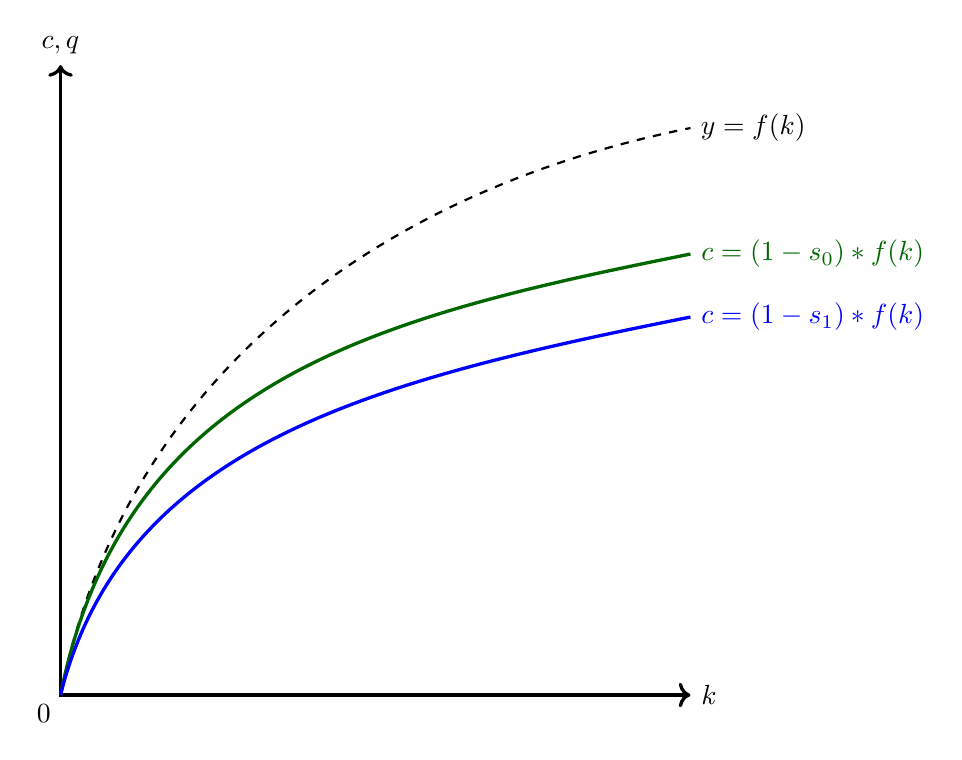
\begin{tikzpicture}[scale=0.8]\label{consumption_function_solow}
\draw[very thick,<->] (0,10) node[above]{$c,q$}--(0,0)--(10,0) node[right]{$k$};
\node [below left] at (0,0) {$0$};
\draw[dashed, thick] (0,0) ..controls (1,5) and (5,8) .. (10,9) node[right]{$y=f(k)$};
\draw[very thick, black!60!green] (0,0) ..controls (1,5) and (5,6) .. (10,7) node[right]{$c=(1-s_0)*f(k)$};
\draw [very thick, blue] (0,0) ..controls (1,4) and (5,5) .. (10,6) node[right]{$c=(1-s_1)*f(k)$};
\end{tikzpicture}
\caption{The Consumption Function the Solow Model and a change in the savings rate}
\end{figure}

Given consumption is a part of total production, the graph for consumption has the same shape as the production function. An increase of the savings rate will push the consumption function down - as $s_1 > s_0$.

\subsubsection*{The dynamics of $k$}
\begin{tcolorbox}[fontupper=\large, fontlower=\normalsize]
\begin{equation}\label{solow_fundamental}
    \dot{k}(t)=sf(k(t))-k(n+g+\delta)
\end{equation}
\tcblower
The Fundamental Equation of The Solow Model
\end{tcolorbox}

\ref{solow_fundamental} is what is refered to as the key equation of the Solow Model. $\dot{k}(t)$ is the growth rate of the capital stock per unit of effective labour, and it depends on the investment per unit of effective labour - $sf(k(t))$ - and the break even level of investment - $k(n+g+ \delta )$ - which is the minimum level of investment needed to maintain a constant level of $k$. Two reasons for this to be break even level of investment:
\begin{itemize}
    \item Existing capital is depreciating, and it must be replaced to keep the capital stock from falling, this is given by $\delta k$
    \item The quantity of effective labour is growing at rate $n+g$, thus keeping the investment constant is not enough to keep the capital stock per unit of effective labour constant, so capital stock must also grow by $n+g$
\end{itemize}
The following graph returns the relation described above:

\begin{figure}[H]
\centering
\begin{tikzpicture}[scale=0.8]
\draw[thick,<->] (0,10) node[above]{$\frac{I}{AL}$}--(0,0)--(10,0) node[right]{$k$};
\node [below left] at (0,0) {$0$};
\draw(0,0)--(9,9) node[right]{$(n+g+\delta) k$};
\draw(0,0) ..controls (1,5) and (5,6) .. (10,7) node[right]{$sf(k)$};
\draw[dashed] (6.1,6.1) -- (6.1,0) node[below]{$k^*$};
\end{tikzpicture}
\caption{Investment in the Solow Model}
\end{figure}

\begin{itemize}
    \item The 45\textdegree line $(n+g+ \delta)k$ represents the break-even level of investment.
    \item The curve $sf(k)$ represents total investment.
\end{itemize}

Given that the optimal level of investment $k^*$ is given by the interception between the two functions, $sf(k)=(n+g+ \delta)k \implies \dot{k}=0$.

\subsubsection{Steady State in the Solow Model (Balanced Growth Path)}

Recall equation \ref{solow_fundamental}, we can define steady state as the long run equilibrium where quantities grow at constant rates. In the Solow model's steady state, $k=k^{*}$. At $k^{*}$ the variables grow at constant rates: 
\begin{itemize}
    \item Labour grows at rate $n$;
    \item Technical progress grows at rate $g$;
    \item Because $K=ALk$, K grows at rate $n+g$;
    \item Since we assume constant returns to scale, $y=f(k)$, will grow at the same rate as $k$, which is the same as the growth rate of $K$, which will be $n+g$;
    \item Output per worker, $\frac{Y}{L}$, and capital per worker, $\frac{K}{L}$, are both growing at the constant rate $g$.
\end{itemize}




\subsubsection*{The Golden Rule of Capital Accumulation}
The Golden Rule of Capital Accumulation ensures that the level of consumption is maxmimized. There exists a level of the savings rate, which maximizes the consumption, denoted as $s_\text{gold}$. The savings rate that reaches this level corresponds to a capital accumulation level $k_\text{gold}$. At $k_\text{gold}$ the capital accumulated is just enough to keep the capital stock constant after depreciation has been subtracted. Thus:

$$f'(k_\text{gold}) = \delta + n + g $$

If we are below $k_\text{gold}$, we can both save more and increase consumption at the steady state, and if we are above we can save less and still increase consumption at the steady state. 

With a Cobb-Douglas production function, the savings rate at the optimal level is $\alpha$. Because $s_{\text{gold}}$ is expressed as:

$$
s_{\text{gold}} = \frac{\text{MPK}}{APK}
$$

\subsubsection*{Dynamic inefficiency}
\begin{itemize}
    \item When the economy is below $k^*_\text{gold}$ , higher saving will increase consumption; when it is above $k^*_\text{gold}$, steady-state consumption can be increased by saving less.
    \item In the latter case, capital-labor ratio is too high so that individuals are investing too much and not consuming enough (dynamic inefficiency).
    
\item  Such dynamic inefficiency will not arise once we endogenous consumption-saving decisions. (Ramsey)
\end{itemize}
\subsubsection{Primary conclusions of the Solow Model}
\begin{enumerate}[i]
\item Simple and tractable framework, which allows us to discuss capital accumulation and the implications of technological progress
  \item Steady state is reached when the growth in the capital stock is just enough to keep the kapital stock per unit of effective labour constant. 
  \item Savings rate $s$ is exogenous and thus dynamic inefficiency can exist.
  \item No sustained growth without technological progress, which in the Solow model is exogenous $g_A$.
  \item Capital accumulation: determined by the saving rate, the depreciation rate and the rate of population growth. All are exogenous
  \item Differences in capital does not sufficiently explain cross-country income differences. 
\end{enumerate}


\begin{figure}
    \centering
    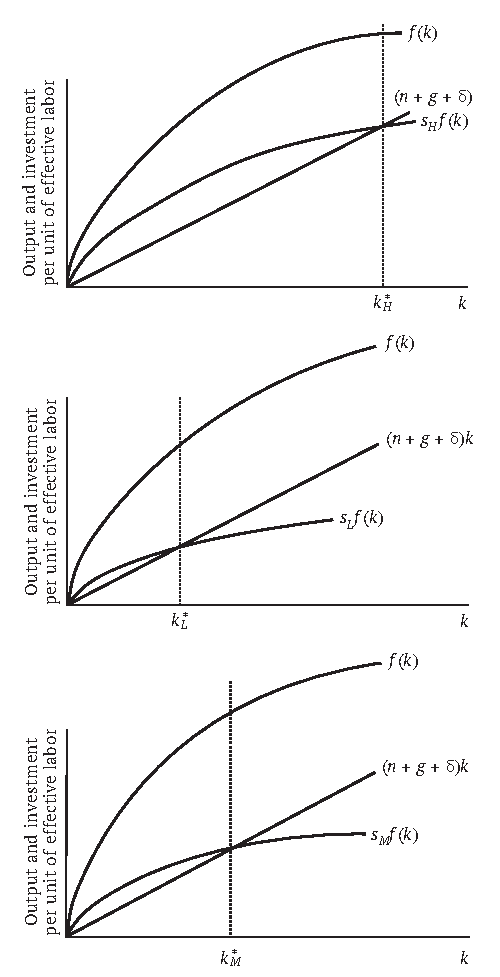
\includegraphics{1_0_Growth_Theory/solow_graphs.pdf}
    \caption{Output investment and consumption along the balanced growth path}
    \label{fig:my_label}
\end{figure}





\newpage
 \section{The Ramsey-Cass-Koopmans model}\label{ramsey-model}
 
 \subsubsection{Assumptions}
\begin{itemize}
    \item Large number of identical firms, each having access to the production function $F(K,AL)$;
    \item Workers and capital are in competitive factor markets, implying they are paid the respective marginal productivity's;
    \item $A$ is given and grows at rate $g$;
    \item As firms are owned by households all profits accrue to them. 
\end{itemize}

\subsubsection{Consumption in the Ramsey Model}

In the Solow Model the consumption was given by an exogenous function. 

\begin{itemize}
    \item $ \bar{H}$ = The total number of households
    \item $ \frac{L(t)}{\bar{H}} $ = Workers per household
\end{itemize}
In continuous time, we have the following maximization problem: 

\begin{equation}
\begin{aligned}
& \underset{x(t)}{\max}
& & \int_{t=0}^{\infty} \rho ^{-\eta t}.V[x(t);S(t)].dt \\
& \text{subject to}
& & \dot{S}(t)= g\left[x(t);S(t)\right]\\
\label{tab:ramsey1}
\end{aligned}
\end{equation}

In discrete time we have the following: 

\begin{equation*}
\begin{aligned}
& \underset{x(t)}{\max}
& &   \sum_{t=0}^{\infty} (1+\eta)^{-t}.V(x_{t};S_{t}) \\
& \text{subject to} 
& & \Delta S_{t+1}=S_{t+1}-S_{t}=g(x_{t},S_{t}) \\ 
& \text{Where}
& & \eta \in (0,1)
\end{aligned}
\end{equation*}

Where $V(t)$ is the Utility Flow, or the Felicity Function which is defined as:

\begin{equation}
    V(t)=u(t)*\frac{L(t)}{\bar{H}}
\end{equation}


\begin{equation}
    u(t)=\frac{C(t)^{1-\theta}-1}{1-\theta} , \theta>0  
\end{equation}

$C(t)$ is the consumption of each household member. 
Considering $L(t)=L(0).e^{nt}=>L(t)=e^{nt}$ because $L(0)=1$. 
Thus we can rewrite \ref{tab:ramsey1} as follows: 

\begin{equation}
\begin{aligned}
 & \underset{U}{\max}
 & & \int_{t=0}^{\infty} e^{(-\rho-\theta.n) t}*\frac{C(t)^{1-\theta}-\rho^{(1-\theta).n.t}}{1-\theta}dt \\
 & \text{subject to} 
 & & \dot{k}(t)=w(t).L(t) + R(t).K(t)-c(t)-\delta K(t) 
\end{aligned}
\end{equation}

The constraint in this case implies that profits are zero. That is because the model assumes competitive markets. 

\paragraph{}

By optimizing through an Hamiltonian we get

\begin{equation*}
    H=\frac{C(t)^{1-\theta}-e^{(1-\theta).n.t}}{1-\theta}+\lambda.(w.L+R.K-c-\delta .K)
\end{equation*}

From this Hamiltonian function we get the optimization conditions, from which we take some conclusions and important functions for the model. 

From the first order condition for K comes: 

\begin{equation}
    \frac{\partial H}{\partial K}=\lambda.(r-\delta)=-\dot{\lambda}+\eta.\lambda \implies \frac{\dot{c}}{c}=\frac{1}{\theta}[(R-\delta)-(\rho - \theta.n)]
\label{tab:euler1}
\end{equation}

This result is very important for this model, and the Diamond model, as it translates the consumption dynamics in the Economy. This is known as the Euler Consumption Function.

From the first order condition for C comes: 

\begin{equation}
\begin{aligned}
& & \frac{ \partial H}{\partial C}=C^{(-\theta)}-\lambda=0 \\
&  \text{because} 
& \lambda=C^{-\theta}
\end{aligned}
\end{equation}

From the first order condition for $\lambda$ comes 

\begin{equation}
    \frac{ \partial H}{ \partial \lambda}=w.L + r.K - c - \delta.K=\dot{K}
\end{equation}

\subsubsection{Variables in the intensive form}
Now rewriting \ref{tab:euler1} in the intensive form:

\begin{equation}
    \frac{\dot{c}}{c}=\frac{f'(k)-(\delta + \rho + \theta.g)}{\theta}
    \label{tab:euler intensive}
\end{equation}

All other variables in the intensive form are like the ones for the Solow model. 

\subsubsection{Consumption dynamics}

We know that a steady state $\dot{c}=0$. Hence, the following condition must apply: 

\begin{equation*}
\begin{aligned}
    f'(k^*)=\rho + \delta + \theta.g \iff\\
 \iff f'(k^*)=\rho + n - n + g - g + \delta + \theta . g \iff \\
  \iff  f'(k)=(n+g+\delta)+[\rho - n - (1-\theta).g]
\end{aligned}
\end{equation*}
\paragraph{}

We know that $(n+g+\delta)$ is equal to $f'(k_{G})$ by the golden rule of capital accumulation and we know that $[\rho - n - (1-\theta).g]$ is positive. Hence, we can infer that $f'(k^*)>f'(k_{G})$ and so $k^*<k_{G}$, demonstrating that there can be no dynamic inefficiency in a Ramsey Economy.

\subsubsection{Capital dynamics}
Capital in the Ramsey model works very much like in the Solow model. It's only worth noting this: 

\begin{equation*}
\begin{aligned}
    \dot{K}=w.L+R.K-C-\delta . K \implies \\
    \implies \dot{k}=f(k)-c-(n+g+\delta)k
\end{aligned}
\end{equation*}

\subsubsection{Steady States}
Any steady state in the Ramsey Model has to comply to the following condition:

\begin{equation*}
    \lim_{t\rightarrow \infty}e^{-(\rho - \theta .n)t}.c(t)^{-\theta}.K(t)=0
\end{equation*}

\subsubsection{System Dynamics}



\begin{equation*}
\begin{aligned}
    \begin{cases} \dot{c}=c.\frac{f'(k)-\delta-\rho-\theta .g}{\theta} \\ 
    \dot{k}=f(k)-(n+g+\delta )k-c
    \end{cases}
\ \implies
\begin{cases}
     \dot{c} \simeq    \frac{f'(k^{*})-\delta-\rho-\theta . g}{\theta}.(c-c^{*})+c^{*}.\frac{1}{\theta}.f''(k^{*}).(k-k^{*}) \\
     \dot{k} \simeq [f'(k^{*}-(n+g+\delta)].(k-k^{*})-(c-c^{*})
\end{cases}
\end{aligned}
\end{equation*}

\paragraph{}
To put in matrix form,

$$    
\begin{bmatrix}
    \dot{c} \\ 
    \dot{k}
\end{bmatrix}
=
\begin{bmatrix}
    0 &  \frac{c^{*}}{\theta}.f''(k^{*}\\
    -1 & f'(k^{*})-(n+g+ \delta)
\end{bmatrix}
.
\begin{bmatrix}
    (c-c^{*}) \\
    (k-k^{*})
\end{bmatrix}
$$

Let 
$
\begin{bmatrix}
    0 &  \frac{c^{*}}{\theta}.f''(k^{*}\\
    -1 & f'(k^{*})-(n+g+ \delta)
\end{bmatrix}$
= $J^{*}$, we can see, then, 

\begin{itemize}
    \item $det(J^{*})=\frac{c^{*}}{\theta}.f''(k^{*})= \lambda_{1}.\lambda_{2} <0$
    \item $tr(J^{*})=f'(k^{*})-(n+g+\delta)=\lambda_{1}+\lambda_{2} >0$
\end{itemize}

From this we can take the equilibrium dynamics, as a graph: 

\begin{figure}[H]
    \centering
    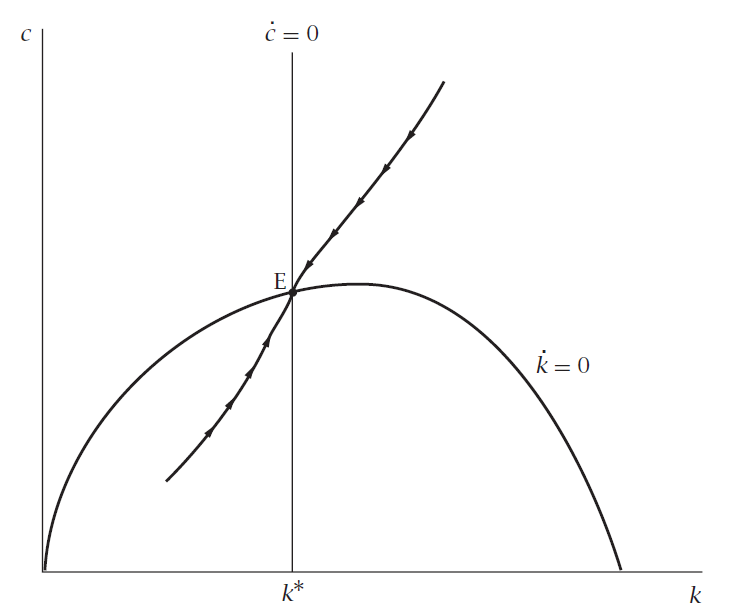
\includegraphics[width=.7\textwidth]{Ramsey.PNG}
    \caption{Ramsey Model Dynamics}
    \label{fig:my_label}
\end{figure}

We can see there is only one stable equilibrium, given by point E, whose equilibrium path we can see by the contract curve. 

The initial point of the economy in terms of consumption and capital accumulation is very important on this model, as it may change the results entirely. 
    \begin{itemize}
        \item If the starting point is between the contract curve and the capital path, it will converge to the contract curve. This will happen on points to the right of E, as well as to the left. 
        \item If the starting point is below the capital accumulation path, to the right of the contract curve, the economy will accumulate capital infinitely, until it reaches a point of zero consumption. This will violate the transversality condition.
        \item If the starting point is above the capital accumulation path, to the left of E, the economy will increase consumption and decrease capital accumulation until it reaches a point of zero capital. This violates the condition $\rho>n+(1-\theta)g$.
        \item We should also note that there is an equilibrium at (0,0), but it is unstable, as a little increase in capital will increase consumption, and this will start a cycle of more consumption - more capital which will end at the stable growth path of the contract curve and eventually point E.
        \item Furthermore the maximum point of the capital accumulation curve $\dot{k}=0$ gives us the golden rule level of capital accumulation, after which increasing capital will only decrease consumption. 
    \end{itemize}

\subsubsection{Fiscal Policy and the government}
For simplicity we'll assume government will take a lump sum tax $T$ (this achieves the same results, without increasing the difficulty of the math if it were a distortionary tax) to finance it's consumption, $G$. Thus equations in the model change as such: 

\begin{equation*}
    \dot{K}=w.L+R.K-T-c-\delta \implies Y=C+I+G
\end{equation*}
We should note that $w.l+R.K=Y$, and $T=G$, which makes government expenditure in this model have a negative impact on total output, by having a negative impact on total capital. 


\paragraph{}
Also,
\begin{equation*}
    \dot{k}=f(k)-c-\gamma-(n+g+\delta).k
\end{equation*}
Where $\gamma=\frac{G}{AL}$

\begin{figure}[H]
    \centering
    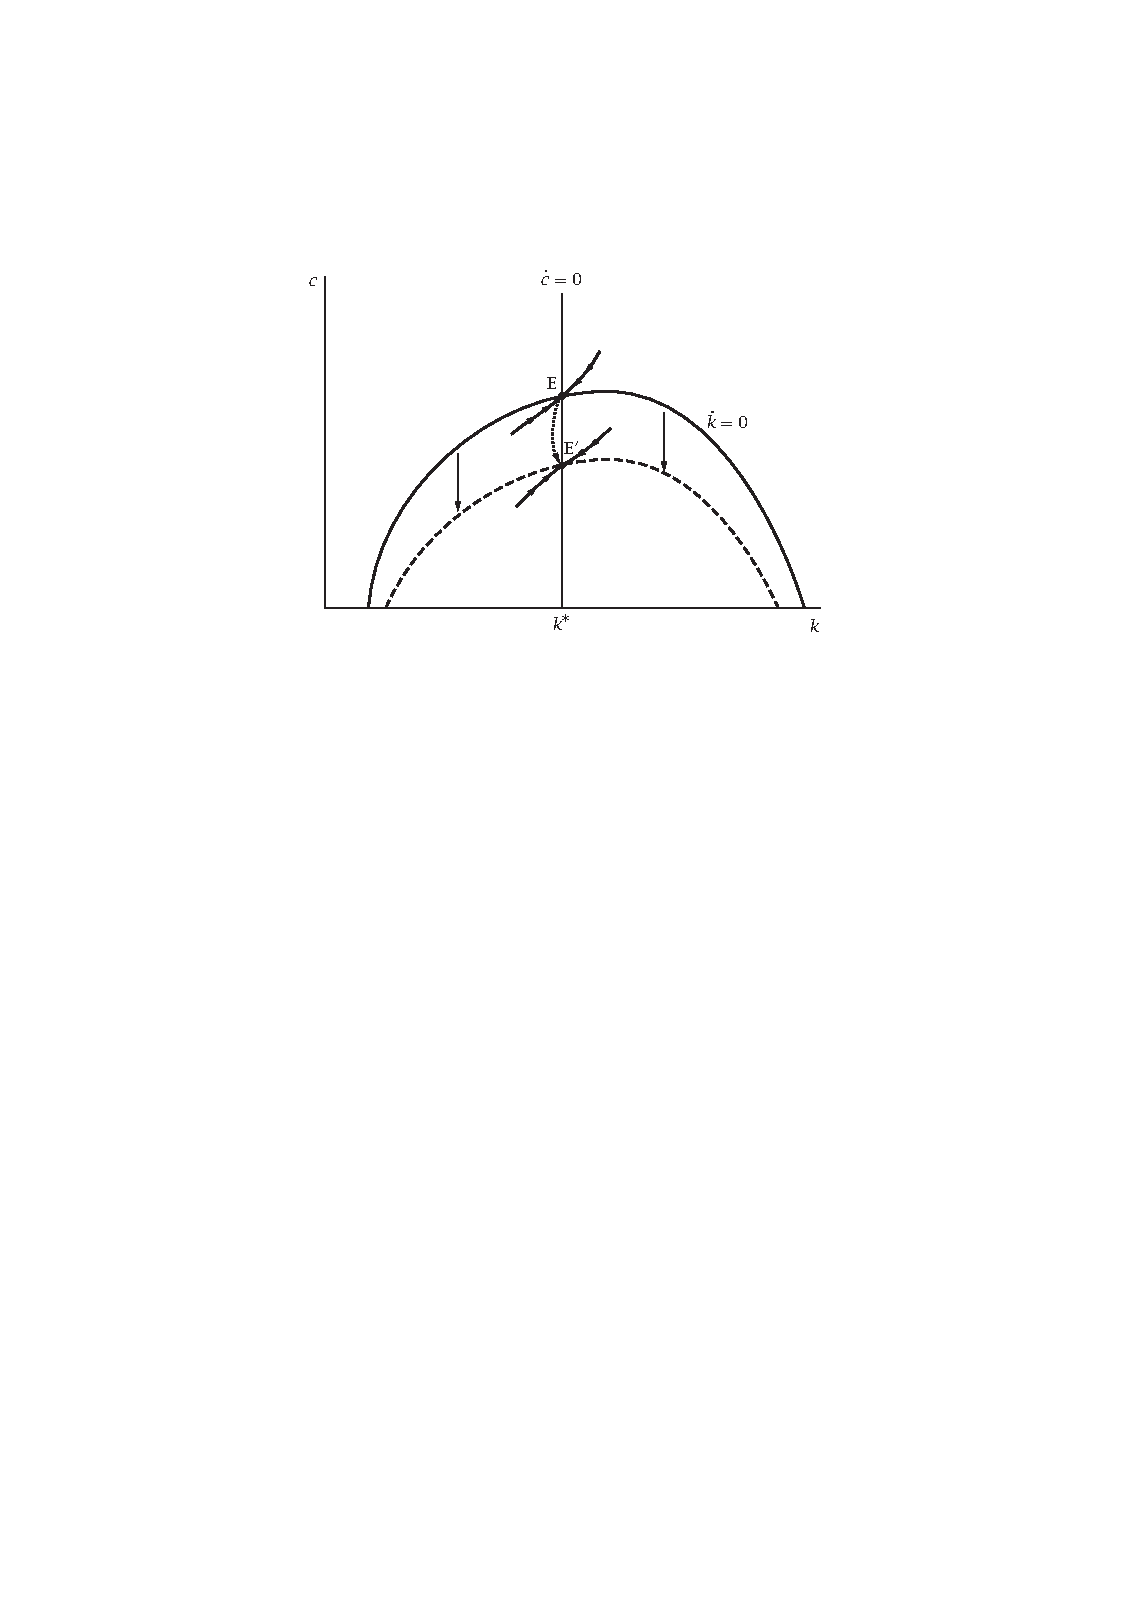
\includegraphics[max width=\linewidth]{1_0_Growth_Theory/RamseyGov.pdf}
    \caption{Government in the Ramsey Model. Source: \textcite{romer_advanced_2012}}  
\end{figure}


Graphically we can see that government expenditure will push the capital accumulation path down, creating a new equilibrium path with lower consumption for the same levels of capital per worker. This is a total crowding out of fiscal policy in a Ramsey Model, because Ricardian Equivalence holds.

\clearpage

\subsection*{Dynamic inefficiency in the Ramsey Model}
As opposed to the Solow model, decisions of savings and consumption in the Ramsey Model is endogenous. Actors will therefore be able to alter their savings and consumption to maximize utility and a dynamic efficiency such as the one we saw in the Solow Model can not exist in the Ramsey Model. The conclusion is slightly different in the OLG-model, mainly because of the assumptions. 

This makes sense given the model's assumptions. If agents are rational, on an infinite time horizon hypothesis, The Ricardian Equivalence\footnote{The Ricardian equivalence proposition is an economic hypothesis holding that consumers are forward looking and so internalize the government's budget constraint when making their consumption decisions. This leads to the result that, for a given pattern of government spending, the method of financing that spending does not affect agents' consumption decisions, and thus, it does not change aggregate demand. Thus, this theorem is used as an argument against tax cuts aimed to boost aggregate demand.} theorem holds, meaning that agents know that any increase in government spending will be need to be financed through future taxes.


\subsubsection{Primary conclusions of the Ramsey Model}
\begin{enumerate}[i]
  \item The steady state is similar to the Solow Model
  \item Saving and consumption decisions are endogenous, and dynamic inefficiency can not exist, because agents are maximizing their utility at any given time given the expectations of the future. 
  \item Countries with higher taxes on investment will have a lower capital stock, lower capital per worker, and lower capital output ratio.
\end{enumerate}
\newpage
\section{The Overlapping Generations (Diamond) model}\label{overlapping-generations-model}
\subsubsection{Introduction}
The Ramsey model is useful for looking at how for instance taxation can affect economic growth++
\subsubsection{General assumptions}
\begin{enumerate}
    \item Offspring does not matter. I.e. nothing is saved for future generations and all newborn generations start with 0 assets.
    \item Households live in 2 periods. One where they are actively contributing in the labor force and another where they are retired and living off savings and returns on investments. I.e. They are young, then they become old before they die. When one generation dies another young generation is born, which is where the name "Overlapping Generations" come from. 
    \item In the Ramsey Model the agents (households) had infinite lives, here households live forever, but the agents that compose the households do not. 
    
\end{enumerate}

\subsubsection{The household utility maximization problem}

\begin{equation}
\begin{aligned}
& \underset{U_t}{\max}
& & U_t=\frac{\mathcal{C}_{1,t}^{1-\theta}-1}{1-\theta}+\frac{1}{1+\rho}*\frac{\mathcal{C}_{2, t+1}^{1-\theta}-1}{1-\theta} & &  \texttt{where} & & \theta > 0  & & \rho > 0
\end{aligned}
\end{equation}

Budget constraint in period 1
\begin{equation*}
    \mathcal{C}_{1, t}+\mathcal{S}_t=W_t*1=A_t*\omega_t*1
\end{equation*}

Budget constraint in period 2
\begin{equation*}
    \mathcal{C}_{2, t+1}=(1+r_{t+1})*\mathcal{S}_t
\end{equation*}

\begin{equation}
    \mathcal{L}=\frac{\mathcal{C}_{1, t}^{1-\theta}-1}{1-\theta}+\frac{1}{1+\rho}*\frac{C_{2, t+1}^{1-\theta}-1}{1-\theta}+\lambda \Bigg[\mathcal{C}_{2, t+1}-(1+r_{t+1})(A_t*\omega_t - \mathcal{C}_{1, t})\Bigg]
\end{equation}

By partial differentiation we can get the following First Order Conditions (FOC) for utility maximization:

\begin{equation*}
    \frac{\partial \mathcal{L}}{\partial \mathcal{C}_{1, t}} = \mathcal{C}_{1, t}^{\theta} + \lambda (1+r_{t+1}) = 0
\end{equation*}

\begin{equation*}
    \frac{\partial \mathcal{L}}{\partial \mathcal{C}_{2, t+1}} = \frac{1}{1-\rho} * \mathcal{C}_{2, t+1}^{-\theta}*\lambda = 0
\end{equation*}

Which we can write as:

\begin{tcolorbox}[fontupper=\large, fontlower=\normalsize]
\begin{equation}\label{consumption_euler_equation}
\frac{\mathcal{C}_{2, t+1}}{\mathcal{C}_{1, t}}= \Bigg( \frac{1+r_{t+1}}{1+\rho} \Bigg)^{\frac{1}{\theta}}
\end{equation}
\tcblower
The Consumption Euler equation in discrete time
\end{tcolorbox}

\begin{equation*}
    \bigg(\frac{1+r_{t+1}}{1+\rho}\bigg)^{\frac{1}{\theta}}\mathcal{C}_{1t}=(1+r_{t+1})(A_{t}\omega_{t}-\mathcal{C}_{1t})
\end{equation*}
\begin{equation*}
    \mathcal{C}_{1t}=\frac{1+r_{t+1}}{1+r_{t+1}\big(\frac{1+r_{t+1}}{1+\rho}\big)^{\frac{1}{\theta}}}A_{t}\omega_{t}
\end{equation*}

Consumption of young individuals in period t. 
\begin{equation*}
    \mathcal{S}_{t}= A_{t}\omega_{t}-\mathcal{C}_{1t}=...=s(r_{t+1})A_{t}\omega_{t}=s(r_{t+1})\omega_{t}
\end{equation*}
\begin{equation*}
    s(r_{t+1})=\frac{(1+r_{t+1})^\frac{1-\theta}{\theta}}{(1+\rho)^\frac{1}{\theta}+(1+r_{t+1})^\frac{1-\theta}{\theta}}
\end{equation*}

Savings as a function of the interest rates of period $t+1$.

\begin{equation*}
    \frac{d s_{t}}{d r_{t+1}}=\frac{1-\theta}{\theta}\bigg(\frac{1+\rho}{1+r_{t+1}} \bigg)^\frac{1}{\theta}s_{t}^2
\end{equation*}

\begin{itemize}
    \item $\theta=1 \implies \frac{ds_{t}}{d r_{t+1}}=0 \implies U_{t}=ln(\mathcal{C}_{1t})+\frac{1}{1+\rho}.ln(\mathcal{C}_{2,t+1})$
    \item $\theta < 1 \implies \frac{ds_{t}}{dr_{t+1}}>0$
    \item $\theta > 1 \implies \frac{ds_{t}}{dr_{t+1}}<0$
\end{itemize}

One should note that $s_{t}$ is the savings rate, taken as endogenous. $\mathcal{S}$ is the savings per household, while $S$ is the total savings in the economy.

Also, $\mathcal{C}_{i,t}$ is the consumption of the group (young or old people) i ($i=1,2$) per household, at time $t$, while $C_{t}$ is the total consumption in the economy at time $t$.

\subsubsection{Capital Accumulation}
\begin{itemize}
    \item $\mathcal{C}_{1t}=W_{t1}-S_{t}$
    \item $\mathcal{C}_{2t}=(1+r_{t})S_{t-1}$
\end{itemize}
\begin{equation}
    K_{t+1} = K_t + W_t  L_t + R_t * K_t - \delta K_t -(L_t*\mathcal{C}_{1t} + L_{t-1}*\mathcal{C}_{2t})
\end{equation}
In the above equation the we can see that the $W_tL_t+R_tK_t=Y_t$, $L_t*\mathcal{C}_{1t} + L_{t-1}*\mathcal{C}_{2t}=C_{t}$, and, $R_{t}=r_{t}+\delta$.
\begin{equation*}
    K_{t+1}=K_{t}+W_{t}L_{t}+(r_{t}+\delta)K_{t}-\delta K_{t}-L_{t}(W_{t}-\mathcal{S}_{t})-L_{t-1}(1+r_{t})\mathcal{S}_{t-1}
\end{equation*}
\begin{equation*}
    K_{t+1}=(1+r_{t+1})(K_{t}-L_{t}\mathcal{S}_{t-1})+L_{t}\mathcal{S}_{t}
\end{equation*}
To see how capital accumulation works, imagine that you're looking at the beginning of times and there is no capital or savings from the previous period (because there is no previous period).

$t=0$
\begin{equation*}
    K_{1}=L_{0} \mathcal{S}_0
\end{equation*}

$t=1$
\begin{equation*}
    K_{2}=L_{1} \mathcal{S}_{1}=S_{1}
\end{equation*}

$t=2$
\begin{equation*}
    K_{3}=L_{2} \mathcal{S}_{2}=S_{2}
\end{equation*}

Hence, 

\begin{equation*}
    K_{t+1}=S_{t}=L_{t}\mathcal{S}_{t}=L_{t}s(r_{t+1})W_{t}=L_{t}s(r_{t+1})A_{t}\omega_{t}
\end{equation*}

Note that $A_{t}=A_{0}(1+g)^t$, and $L_{t}=L_{0}(1+n)^t$.

The function for capital per unit of effective labour accumulation comes as:

\begin{equation*}
    k_{t+1}=\frac{K_{t+1}}{A_{t+1}L_{t+1}}=\frac{L_{t}s(r_{t+1})A_{t}\omega_{t}}{A_{t+1}L_{t+1}}=\frac{L_{t}s(r_{t+1})A_{t}\omega_{t}}{A_{t}(1+g)L_{t}(1+n)}=\frac{s(r_{t+1})\omega_{t}}{(1+g)(1+n)}
\end{equation*}

Workers are remunerated by their marginal product: 

\begin{equation*}
    w_{t}=MPL_{t} \implies A_{t}\omega_{t}=A_{t}\big[f(k_{t})-k_{t}f'(k_{t}) \big]
\end{equation*}

Also, capital is paid it's marginal product: 

\begin{equation*}
    R_{t}=MPK_{t} \implies r_{t+1}+\delta=f'(k_{t+1}) \implies r_{t+1}=f'(k_{t+1})-\delta
\end{equation*}
\begin{equation*}
   \implies k_{t+1}=\frac{1}{(1+g)(1+n)}s(f'(k_{t+1})-\delta)\big[f(k_{t})-k_{t}f'(k_{t}) \big]
\end{equation*}

Say $k_{t+1}=h(k_{t},\overline{n},\overline{g},\delta)$, and $\beta=\frac{1}{(1+g)(1+n)}$.

\begin{equation*}
    \frac{\partial k_{t+1}}{\partial k_{t}}=\frac{s_{t}\beta k_{t}f''(k_{t})}{1-\beta s'(r_{t+1})f''(k_{t+1})\omega_{t}}
\end{equation*}

\subsubsection{Long-run Equilibrium}

\subsubsection{A particular case}
\begin{itemize}
    \item Cobb-Douglas production function $y_{t}=k_{t}^{\alpha} \implies f'(k_{t})=\alpha k_{t}^{\alpha-1}$
    \item Logarithmic Utility $\theta=1 \implies s=\frac{1}{2+\rho} \implies s'=0$
\end{itemize}

\begin{equation*}
   k_{t+1}= \frac{1}{(1+n)(1+g)}\frac{1}{2+\rho}\bigg[ k_{t}^\alpha-k_{t}k_{t}^{\alpha-1}\alpha \bigg]
\end{equation*}

\begin{equation*}
    k_{t+1}=\frac{1-\alpha}{(1+n)(1+g)(2+\rho)}k_{t}^{\alpha} \implies k^{*}=\bigg[\frac{1-\alpha}{(1+n)(1+g)(2+\rho)} \bigg]^{\frac{1}{1-\alpha}}
\end{equation*}

\begin{equation*}
    \frac{\partial k_{t+1}}{\partial k_{t}} \bigg \rvert_{k_{t}=k^*}=\frac{1-\alpha}{(1+n)(1+g)(2+\rho)}\alpha k^{\alpha-1}=\alpha \in ]0, 1[
\end{equation*}

\subsubsection{Dynamic inefficiency in the OLG Model}
\begin{equation*}
    K_{t+1}=(1-\delta)K_{t}+Y_{t}-C_{t}
\end{equation*}
\begin{equation*}
    \frac{K_{t+1}}{A_{t}L_{t}}=(1-\delta)k_{t}+y_{t}-c_{t}
\end{equation*}
\begin{equation*}
    (1+g)(1+n)k_{t+1}=(1-\delta)k_{t}+f(k^*)-c_{t}
\end{equation*}
\begin{equation*}
    c_{t}^*=\big[(1-\delta)(1+g)(1+n)\big]k^{*}+f(k^*)
\end{equation*}
\begin{equation*}
    f'(k_{G})=\delta+(1+g)(1+n)-1
\end{equation*}
\begin{equation}
    k_{G}=\bigg[\frac{\delta+(1+g)(1+n)-1}{\alpha}\bigg]^{\frac{1}{1-\alpha}}
\end{equation}
\begin{equation}
    k^*=\bigg[ \frac{1-\alpha}{(1+n)(1+g)(2+\rho)} \bigg]^{\frac{1}{1-\alpha}}
\end{equation}

So can there be dynamic inefficiency in an OLG model? Yes. There is no guarantee that $k^*<k_{G}$, it depends on the values of the exogenous growth rates of which $k^*$ and $k_{G}$ depend. Dynamic inefficiency in the OLG-model can be alleviated with a pension scheme.

\subsubsection{Social Security - Pensions}
First Recall the entire model, this time, with government.

\begin{equation}
    \frac{\mathcal{C}_{2,t+1}}{\mathcal{C}_{1t}}=\bigg(\frac{1+r_{t+1}}{1+\rho}\bigg)
\end{equation}
\begin{equation}
    \mathcal{C}_{1t}=W_{t}-(\mathcal{S}_{t}+d_{t})
\end{equation}
\begin{equation}
    \mathcal{C}_{2,t+1}=(1+r_{t+1})\mathcal{S}_{t}+b_{t}
\end{equation}
\begin{equation}\label{Cap_acc_OLG}
    K_{t+1}=(1-\delta)K_{t}+W_{t}L_{t}(r_{t}+\delta)K_{t}-L_{t}\mathcal{C}_{1t}-L_{t-1}\mathcal{C}_{2t}
\end{equation}
\begin{equation}
    W_{t}=A_{t}\bigg[ f(k)-k_{t}f'(k_{t})\bigg]
\end{equation}
\begin{equation}
    r_{t}=f'(k_{t})-\delta
\end{equation}
\begin{equation*}
    \implies K_{t+1}=(1+r_{t})(K_{t}-L_{t-1}\mathcal{S}_{t-1})+L_{t}(\mathcal{S}_{t}+d_{t})-L_{t-1}b_{t}
\end{equation*}

Note that $b_{t}=d_{t}$ (one agents tax is another's benefit - no deficits, no surplus).

The pension system can be one of two types: fully funded, or pay-as-you-go. 

\subsubsection{Fully Funded}
\begin{equation}
    b_{t}=(1+r_{t})d_{t-1}
\end{equation}

$t=0$
\begin{equation*}
    K_{1}=(1+r_{0})(K_{0}-L_{-1}\mathcal{S}_{-1})+L_{0}(\mathcal{S}_{0}+d_{0})-L_{-1}(1+r_{0})d_{-1}=L_{0}(\mathcal{S}_{0}+d_{0})=L_{0}\Sigma_{0}
\end{equation*}

$t=1$
\begin{equation*}
    K_{2}=(1+r_{1})(K_{1}-L_{0}\mathcal{S}_{0})+L_{1}(\mathcal{S}_{1}+d_{1})-L_{0}(1+r_{1})d_{0}=L_{1}(\mathcal{S}_{1}+d_{1})=L_{1}\Sigma_{1}
\end{equation*}

Hence, replace \ref{Cap_acc_OLG}, by the following equation:
\begin{equation*}
    (1+n)(1+g)L_{t}A_{t}k_{t+1}=L_{t}\Sigma_{t} \implies (1+n)(1+g)A_{t}k_{t+1}=\Sigma_{t}
\end{equation*}
\begin{equation*}
    \mathcal{C}_{1t}=W_{t}-\Sigma_{t}
\end{equation*}
\begin{equation*}
    \mathcal{C}_{2,t+1}=(1+r_{t+1})\Sigma_{t}
\end{equation*}

\begin{equation*}
    \begin{aligned}
        d_{t}<\mathcal{S}_{t}\bigg \rvert_{without SS} \implies \mathcal{S}_{t}\bigg\rvert_{with SS}>0
    \end{aligned}
\end{equation*}

\subsubsection{Pay-as-you-go}
\begin{equation*}
    L_{t-1}b_{t}=L_{t}\frac{b_{t}}{1+n}=L_{t}\frac{1+n}{1+n}d_{t}=L_{t}d_{t}
\end{equation*}
\begin{equation*}
    K_{t+1}=(1+r_{t})(K_{t}-L_{t-1}\mathcal{S}_{t-1})+L_{t}(\mathcal{S}_{t}+d_{t})-L_{t}d_{t}=(1+r_{t})(K_{t}-L_{t-1}\mathcal{S}_{t-1})+L_{t}\mathcal{S}_{t}
\end{equation*}

Using the same type of rationale, replace \ref{Cap_acc_OLG}, by the following equation: 
\begin{equation*}
    (1+n)(1+g)A_{t}K_{t+1}=\mathcal{S}_{t+1}
\end{equation*}

\begin{equation*}
    (1+r_{t+1})d\mathcal{S}_{t}+(1+n)dd_{t+1}=\bigg(\frac{1+r_{t+1}}{1+\rho}\bigg)^{\frac{1}{\theta}}(d\mathcal{S}_{t}-dd_{t})
\end{equation*}

\begin{equation*}
    \frac{d\mathcal{S}_{t}}{d d_{t}}=-\frac{1+n+\beta_{t+1}}{1+r_{t+1}+\beta_{t+1}}<0
\end{equation*}

Where, $\beta_{t+1}=\big(\frac{1+r_{t+1}}{1+\rho}\big)^{\frac{1}{\theta}} $

\begin{equation*}
    r_{t}=f'(k)-\delta
\end{equation*}
\begin{equation*}
    W_{t}=A_{t}\bigg[ f(k_{t})-k_{t}f'(k_{t})\bigg]
\end{equation*}

\begin{equation*}
    d^*\nearrow \implies f^*\searrow \implies k^*\searrow \implies W^*\searrow
\end{equation*}

If we assume that $\frac{d K_{t+1}}{d K_{t}}<0$, then, $\frac{dk^*}{d d^*}<0$




\subsubsection{Primary conclusions of the OLG Model}
\begin{enumerate}[i]
  \item Steady state is reached when ...
  \item Saving and consumption decisions are endogenous, but dynamic inefficiency can still exist.
  \item Equilibria may be "dynamically inefficient" feature overaccumulation: unfunded Social Security can ameliorate the problem.
\end{enumerate}
\newpage
\section{Endogenous growth}\label{learning-by-doing}
\subsubsection{Introduction}
In the previous models we assumed that technical progress, which is one of the main factors of growth were exogenous. This does not sufficiently explain economic growth as a result of innovation and technical progress. 

\subsubsection{General assumptions}
\begin{enumerate}
    \item Experience creates more efficient ways of producing with the same amount of input
    \item New knowledge is a by-product of capital investment into machines
        \begin{itemize}
            \item Workers can learn how to be more efficient with new equipment
            \item Investment in capital units such as machines drives increase in technical progress through the learning by doing process
        \end{itemize}
    \item Knowledge is a pure public good i.e. non-rival and non-excludable. In other words, once knowledge and experience is found one cannot prohibit others from using the same knowledge. 
    \item Perfect Competition, identical firms. 
\end{enumerate}

\subsubsection{The firms}

\begin{equation}
    A(t)=\Lambda \Big[ K(t), L(t) \Big]
\end{equation}

\begin{equation*}
    Y_i = F(K_i, AL_i)
\end{equation*}

\begin{equation*}
   y_i = AL_i \cdot f(k_i)
\end{equation*}

\begin{equation*}
    \pi_i = AL_i \cdot f(k_i) - RK_i - WL_i \\
    \implies \Pi_i = AL_i \cdot f(k_i) - RK_i - WL_i = 
\end{equation*}

\begin{equation*}
    \frac{\partial \pi_i}{L_i} = A \cdot f(k_i) - R \cdot k_i \cdot A - W = 0
\end{equation*}

\begin{equation*}
    \frac{\partial \pi_i}{k_i} = A \cdot Li \cdot f'(k) -  R \cdot L_i \cdot A = 0 \implies f'(k_i) = R 
\end{equation*}

\begin{equation*}
    W=A \bigg[ f(k_{i})-k_{i}f'(k_{i}) \bigg]
\end{equation*}

\begin{equation*}
    Y=\sum_{i=1}^{e}=eF(K_{i},AL_{i})=F\bigg[ ek_{i}, A(eL_{i})\bigg]=F(K,AL)
\end{equation*}

\begin{equation*}
\begin{aligned}
    y=\frac{Y}{AL}=f(k) && \text{Where, }  k=k_{i}
\end{aligned}
\end{equation*}

\begin{equation*}
    R=\frac{\partial F}{\partial K}(K_{i},AL_{i})=\frac{\partial F}{\partial K}\bigg( (eK;A(eL)\bigg)=\frac{\partial F}{\partial K}(K;AL)=f'(k)
\end{equation*}



\begin{equation}
    \dot { K } = Y - C = a k - Z ( t )
\end{equation}

\begin{align}
   a - \bar{g}_c > 0
&&
\beta = 0 
\end{align}


\subsection{The AK Model}

\subsubsection{Some Simplifications}
\begin{itemize}
    \item $\delta=0$
    \item $F(\cdot)$ is Cobb-Douglas
\end{itemize}

\begin{equation*}
    A=a^{\frac{1}{1-\alpha}}\frac{K}{L}
\end{equation*}

\subsubsection{"Solow" Version}


$a>0$, and so, it's implied that more capital will increase technical progress. 

We assume that $n=0$, so population is stable. 

\begin{equation*}
    Y=K^\alpha(AL_{0})^{1-\alpha}=K^\alpha\bigg(a^{\frac{1}{1-\alpha}}\bigg)^{1-\alpha}=aK^{\alpha+1-\alpha}=aK
\end{equation*}

\begin{equation*}
    S=sY=s\cdot a \cdot K
\end{equation*}

\begin{equation*}
    \Dot{K}=S=Y-C=s \cdot a \cdot K
\end{equation*}

\begin{equation*}
    g_{k}=\frac{\Dot{K}}{K}=sa
\end{equation*}

\subsubsection{"Ramsey" Version}

\begin{align*}
    \frac { \dot{C}} { C } = \frac { R - \rho } { \theta }=\frac{\alpha \cdot a - \rho}{\theta} && 
    g_{C}=\frac{\dot{C}}{C}=\frac{\alpha \cdot a -\rho}{\theta}=\overline{g}_{C}
\end{align*}

\begin{equation*}
    R=MPK=\alpha K^{\alpha-1}(AL_{0})^{1-\alpha}=\alpha\bigg(\frac{AL_{0}}{K} \bigg)^{1-\alpha}=\alpha \bigg(\frac{a^{\frac{1}{1-\alpha}}\frac{K_{0}}{L_{0}}L_{0}}{K_{0}} \bigg)^{1-\alpha}=\alpha \cdot a
\end{equation*}

Define consumption as: 
\begin{equation*}
    C(t)=C_{0}e^{\overline{g}_{C}t}
\end{equation*}

\begin{equation*}
    \dot{K}=Y-C=aK-C(t)
\end{equation*}

\begin{equation*}
    K(t)=\frac{C_{0}\cdot e^{\overline{g}_{C}\cdot t}}{a-\overline{g}_{C}}+\beta C^{at}
\end{equation*}


Transversality condition:

\begin{equation*}
    \lim_{t \to \infty} \bigg \{K(t)e^{-rt} \bigg \}=0 \implies \lim_{t \to \infty} \bigg\{ \beta e^{(a-\overline{r})t}+\frac{C_{0}e^{(\overline{g}_{C}t}}{a-\overline{g}_{C}} \bigg\}=0
\end{equation*}

\begin{enumerate}
    \item $a-\overline{g}_{C}>0$
    \item $\beta = 0 $
\end{enumerate}

\begin{equation*}
    K(t)=\frac{C_{0}\cdot e^{\overline{g}_{C}\cdot t}}{a-\overline{g}_{C}} \implies g_{K}=\overline{g}_{C}
\end{equation*}

\input{1_0_Growth_Theory/1_5_2_Learning_By_Doing.tex}










\chapter{The New Classical School}

\section{Adaptive and Rational Expectations}
\textbf{Adaptive Expectations:}
\begin{equation*}
    \textbf{AE:} \ X^{e}_{t+1} = f(X_{t}, X_{t+1}, X_{t+2} \dots X_{t+n})
\end{equation*}

Adaptive Expectations are based on backwards looking data to formulate expectations. 
\\

\textbf{Rational Expectations:}
\begin{equation*}
    \textbf{RE:} \ X^{e}_{t+1} = E(X_{t+1}\mid \Omega_t )
\end{equation*}

Where $\Omega$ is the information set which includes some model of the economy built on the best information available. 

Adaptive expectations are backwards looking, while rational expectations are forward looking.

\section{The Lucas Supply Function and Imperfect Information}
\textbf{The Archipelago economy:}
Each island has a household $i$ and it produces a good $i$ with labour as the only input. Each island is specialized and produces a different good. This good is sold on the weekly marketplace and therefore production decisions needs to be made ahead of time. Every island only has partial information regarding the production of other islands. Everybody is ill informed, but all islands are equally ill-informed.  \\

A simple linear production function with labour as the only input:
\begin{equation*}
    Y_i = 1 \cdot L_i
\end{equation*}

Utility maximization problem: 
\begin{equation*}
\begin{aligned}
& \underset{C, L}{\max}
& & U_i = C_i - \frac{L_{i}^{\gamma}}{\gamma} \\
& \text{s.t}
& & \sum^{n}_{j = i} c_i p_j = p_i * y_i
\end{aligned}
\end{equation*}
The utility function is linear on consumption, but non-linear on labour, because we have $\gamma > 1$ and disutility of labour. 


The consumption basket for household $i$ is:
\begin{equation}
    C_i = C_i \left( c_1^{i}, c_2^{i} ...., c_n^{i}  \right)
\end{equation}
The consumption basket is a homothetic function 


$$
\sum_{j = 1 }^{n} c_j^{i} \cdot p_j = P^{i} C_i
$$

Where $P_i$ is  the price index for the respective household, which is a function written as: 
$$
P^{i} = P^{i} (p_1, p_2, ...., p_n)
$$

The maximization problem is then to maximize production to maximize the expected utility given the information set:
\begin{equation*}
\begin{aligned}
& \underset{Y_j}{\max}
& & E \left[ \frac{p_i}{P} y_j - \frac{y^{\gamma}}{\gamma} \bigg\rvert \Omega \right] = E_i U_i
\end{aligned}
\end{equation*}

Where $P$ is the aggregate price index. 

Jensens inequality: 
$$
E_iY_i^\gamma > (E_iY_i)^\gamma
$$


$$
E_i \left( \frac{P_i}{P} Y_i  \right) = E \left( \frac{p_i}{P}  \right) \cdot E(Y_i) + \text{cov}\left( \frac{p_i}{p} \right)
$$

\begin{equation*}
\begin{aligned}
& \underset{Y_i}{\max}
& & \frac{p_i}{P} y_i - \frac{Y_i^{\gamma}}{\gamma}
\end{aligned}
\end{equation*}

FOC:
$$
\frac{\partial U_i}{\partial Y_i} = \frac{p_i}{P} - Y^{\gamma - 1} = 0 \implies Y^S_i = \left( \frac{p_i}{P^e} \right)^\frac{1}{\gamma - 1 }
$$

Where $Y_i^S$ is the supply of good $i$

This is the Lucas supply function in levels.



\paragraph{Lucas Supply Function in logs}

Lower case denotes variables in log-form.

$$y _ { i } ^ { s } =  \frac{1}{ 1 - \gamma} \left( p _ { i } - p ^ { e }  \right)     $$

The smaller the $\gamma$, the bigger the effect the effect of the relative price the supply decision.

\paragraph{Lucas Demand Function in logs}
\begin{align*}
    y_i^d = y \cdot Z_i \left( \frac{p_i}{p}  \right)^{- \eta} && \text{Where} \ \eta > 0
\end{align*}
$\eta > 0$ is an elasticity 

$$
z_i = \ln Z_i \sim N(0, V_z)
$$

The log of $Z_i$ follows a normal distribution with mean 0 and a finite variance $V_Z)$. Which is an idiosyncratic shock that only affects a specific island.  

$$
y^d_i = y + z_i - \eta (p_i - p)
$$

No expectations, because the demand does not depend on that. Demand is formed when prices are observed at the market. 


The aggregate demand function is given by this very simple equation:
The quantity of money times the velocity, equals the nominal output:
$$
M - V = P \cdot Y
$$

We are assuming that $V = 1$ to simplify, and we have no government and only a central bank that issues money. 

If we write as logs we get:

\begin{equation}\label{lucas_agg_demand}
    y^d = m - p
\end{equation}


\subsubsection{Solution with perfect information}

\begin{align*}
    y^s_i = y^d_i \implies \\
    &&& \frac{1}{\gamma - 1} (p_i - P) = y + z_i - \eta (p_i - P)
\end{align*}

Solve the equation for $p_i$ to get:

$$
p_i = \frac{\gamma - 1}{1 + \eta (\gamma -1)} (y + z_i) + p
$$

All islands are the same, so the above is true for island $i$, but also for the average. In this case, $z$ becomes 0 because different positive and negative shocks cancel each-other out. 

\begin{equation*}
    p = \frac{\gamma - 1}{1 + \eta (\gamma -1)}y + p \implies \emptyset \implies Y
\end{equation*}

Since we are looking at logs, $\emptyset$ does not mean that we are producing no units, but that the economy is at its potential output. We can define $\emptyset = Y^N$ for natural output.

If output is equal to $\emptyset$ the price level will be $M$. If there is a change in money supply prices would go up as much as the increase in money supply, thus if the monetary policy is anticipated there are no real effects on output of changes in monetary policy. 

\paragraph{Solution with imperfect information}

$$
y_i = \frac{1}{\gamma - 1} (p_i - p^e)
$$

Where $(p_i - p^e) = E_i r_i$, $r_i$ is the relative price, the expected value of the relative price given the information set:
$$
E_i r_i = E \left( p_i - P \bigg\rvert \Omega  \right)
$$

\paragraph{Idiosyncratic shocks}
Idiosyncratic shocks is the only thing that can affect the expectations of relative prices. From before we have the individual idiosyncratic shocks given by $z_i$
$$
z_i \approx N(0, V_z)
$$


\paragraph{Aggregate shocks}
We assume that aggregate shocks are only monetary shocks:

$$
m \approx (E(m), V_m)
$$

$$
p_i = p + r_i = p + (p_i - p)
$$


Extracting noise:
$$
E_i r_i = \alpha + \beta p_i
$$


$$
\alpha = - \frac{V_{r}}{V_{r} + V_p} E(p)
$$


$$
\beta = \frac{V_{r}}{V_{r} + V_p}
$$

The variances of relative and aggregate prices. 


Since $\beta = -\alpha \cdot E(p)$ we can rewrite into:

$$
E_i r_i = \beta \left[  p_i - E(p)  \right]
$$

We can substitute this into the Lucas Supply Function:

$$
y_i = \frac{1}{\gamma - 1} \cdot \beta \left[  p_i - E(p)  \right] = b \left[  p_i - E(p)  \right]
$$

Where $b = \tfrac{\beta}{\gamma - 1}$
\subsection*{Lucas Aggregate Supply Function}

Aggregate supply:
\begin{equation*}
   y^s = b [ p - E ( p ) ] 
\end{equation*}

Recall the Lucas Aggregate Demand function in equation \ref{lucas_agg_demand} to find the equilibrium:

$$
y^d = y^s \implies
m - p = b [ p - E( p ) ]
$$

Solving for $p$ gives: 
$$
p = \frac{1}{1+b}m + \frac{b}{1 + b}E(p)
$$

Thus we see that the actual aggregate price level depends on the money supply and the expectations of price. 

\begin{tcolorbox}
The expected value of the expected value is the expected value!
\end{tcolorbox}

The best expectation of $p$:
$$
E(p) = E(m)
$$

$$
m = E(m) + \left[  m - E(m) \right] 
$$

$$
p = \frac{1}{1 +b} \left[ E(m) + [m - E(m)] \right] + \frac{b}{1 + b} E(m) \implies E(m) + \frac{1}{1 + b} \left[ m - E(m) \right]
$$


Substituting into the Lucas Supply Function gives:
$$
y = b \Bigg\{ E(m) + \frac{1}{1 + b} [m - E(m)] - E(m) \Bigg\}
$$

Which simplifies into:

\begin{align}
        y = \alpha [m - E(m)] && \alpha = \frac{b}{1 + b}
\end{align}



\clearpage

\section{Economic policy effectiveness and the Lucas critique}


\subsection{Neutrality of Anticipated policy}

If Monetary policy is anticipated there will be no effect on output or real wages --- the only effect will be on prices. For fiscal policy, the result will be the same. Thus, only \textit{unanticipated} policy changes can have real effects. 

Let us look at how to effectiveness of policy can be independent of the above conclusion. If you introduce rational expectations into a Keynesian model, the results become even more "Keynesian". Rational expectations are not enough to only have surprise effects.

$$
\frac { \partial \alpha_0 } { \partial b } = \frac { \alpha } { 1 + b } > 0
$$

The bigger the $b$, the $\alpha$ is the effect of the surprise component of monetary policy on output.

$$
b = \frac { 1 } { \gamma - 1 } \beta = \frac{1}{\gamma - 1} \frac { V_R } { V _ { R } + V _ { p } }
$$


\begin{align}
     p = E ( m ) + \frac { 1 } { 1 + b } \left[  m - E ( m ) \right] &&
    V_p = V \left( \frac{m}{1 + b} \right) = \frac{V_m}{(1+b)^2}
  \end{align}
  

$$
y _ { i } = y + z _ { i } - \eta\left( p _ { i } - p \right)
$$

Substituting the Lucas Supply function for $y$ yields:

$$
y _ { i } = b [ p - E( p ) ] + z _ { i } - \eta\left( p _ { i } - p \right) \implies b [ p - E( p ) ] - \eta (p_i - p) + Z_i $$

$$
\frac{p_i - p}{r_i} = \frac{Z_i}{b + \eta} \implies V_R = \frac{V_Z}{(b + \eta)^2}
$$




$$
b = \frac{1}{r - 1} \cdot \beta = \frac{1}{\gamma - 1} \cdot \frac{V_R}{V_R + V_p}= \frac{1}{\gamma - 1} \cdot \frac{1}{1 + f(b) \cdot \frac{V_m}{V_Z}}
$$

Where $\tfrac{V_m}{V_z} = R_V$

\begin{align*}
  f ( b ) = \left( \frac { \eta + b } { 1 + b } \right) ^ { 2 }  
\end{align*}

Where $$ \frac { d b } { d R _ { V } } < 0$$, for $\eta \leq 9$ is the relative variance between aggregate and idiosyncratic shocks. The bigger the relative variance, the smaller $b$ will be and thus the impact of surprise policy on output will be smaller. 

The more often aggregate shocks happen, the less effect surprise policy has on the aggregate output. The more often we have idiosyncratic shocks relative to aggregate shocks, the more effective surprise policy will be. 

\subsection{The Lucas Critique}

\[ 
\left\{
\begin{array}{l l}
    y^S=b(p-p^e) \\
    y^d=\theta(m-p)+u
\end{array}
\right.
\]


\begin{align*}
    y=b \bigg( \frac{\theta}{b+\theta}m+\frac{b}{b+\theta}p^e+\frac{u}{b+\theta}-p^e \bigg) \\
    y=-\frac{b\theta}{b+\theta}p^e+\frac{b\theta}{b+\theta}m + \frac{b}{b+\theta}u
\end{align*}

Where $p^e=E(p)$. 

To understand the Lucas critique take the solutions of the model under to regimes of expectations. 

\subsubsection{Static Expectations}

Under static expectations, agents expect for any period, that the price will be equal, or at least related, to the one of the previous period, hence: 

\begin{equation*}
    p_t^e=p_{t-1}
\end{equation*}

So, one would estimate the mode in it's reduced form: 

\begin{equation*}
    y_t=a_0+a_1m_t+a_2p_{t-1}+v_t
\end{equation*}

With the parameters $a_i$ representing the parameters of the extensive form, 

\begin{align*}
    \Tilde{a}_{0}=0 && \Tilde{a}_{1}=\frac{b\theta}{b+\theta} && \Tilde{a}_2=-\frac{b\theta}{b+\theta}
\end{align*}

\subsubsection{Rational Expectations}

\begin{equation*}
    p^e=E(p)
\end{equation*}

Suppose there's a policy rule, $m=\overline{m}-\delta(y-y^n)$ (with $y^n=0$). 

\begin{equation*}
    E(p)=\frac{\theta}{b+\theta}E(m) + \frac{b}{b+\theta}E(p)+\frac{1}{b+\theta}E(u) \implies E(p)=E(m)
\end{equation*}

\begin{equation*}
    E(m)=E[(\overline{m})-\delta y]=\overline{m}-\delta E(y)
\end{equation*}

\begin{equation*}
    E(y)=\frac{b\theta}{b+\theta}\bigg[E(m)-E(p) \bigg]=0
\end{equation*}

\begin{equation*}
    y=-\frac{b\theta}{b+\theta}\overline{m}+\frac{b\theta}{b+\theta}m+\frac{b}{b+\theta}u
\end{equation*}

By estimation, one would get the parameters: 

\begin{align*}
    \hat{a}_0=-\frac{b\theta}{b+\theta}\overline{m} && \hat{a}_1=\frac{b\theta}{b+\theta} &&\hat{a}_2=0
\end{align*}

The problem relies on the fact that under rational expectations, the parameter $\hat{a}_0$ depends on the level $\overline{m}$, and this makes estimation biased and unreliable. 

In terms of econometrics, Lucas suggests the following: 

\begin{itemize}
    \item Using simultaneous equations models of reduced forms;
    \item Estimating parameters through microeconometrics, because it's more reliable. One should, however, consider the limitations of microeconometrics in estimating macro variables. 
\end{itemize}

The Lucas Critique is, in essence, a critique on policymakers. Lucas says expectations are likely to be important to many relationships among aggregate variables, and changes in policy are likely to affect those expectations. 

If all policymakers attempt to take advantage of statistical relationships, effects operating through expectations may cause relationships to break down. 


\section{Economic Policy effectiveness}

\paragraph{The Conservatice Central banker}

$$
\epsilon_{\text{GCB}} > \epsilon
$$

$$
\frac{\partial \Pi_m}{\partial \epsilon} - \frac{b}{\epsilon^2}y^* < 0
$$





\newpage
\input{2_0_New_Classical_School/2_2_Imperfect_Information_Lucas_Supply.tex}
\newpage






\newpage
%\section{Economic Policy effectiveness}

%\paragraph{The Conservatice Central banker}

%$$
%\epsilon_{\text{GCB}} > \epsilon
%$$

%$$
%\frac{\partial \Pi_m}{\partial \epsilon} - \frac{b}{\epsilon^2}y^* < 0
%$$
\chapter{Real Business Cycles}
\section{Trend and business cycle: short-run stylised facts}


\subsubsection{Trends and cycles revisited}

\begin{center}
\begin{tikzcd}
 & X_{t}^{*} \arrow[r] & \text{Trend Component} \\
X_t \arrow[ru, no head] \arrow[rd, no head]  \\
 & \Tilde{X_t} \arrow[r]  & \text{Cyclical Component}
\end{tikzcd}
\end{center}

$$
\Tilde{X_t} = ln X_t - ln X_{t}^{*}
$$

Filters

\begin{enumerate}[a)]
    \item Variability of the standard deviation:
    $$
        \Tilde{X}_t = \frac{\sigma \Bar{x}}{\sigma \Bar{y}}
    $$
    
    \item
    Cyclicality 
    
    $$
    \text{Corr}\left( \Tilde{Y}_t, \Tilde{X}_{t + k} \right)
    $$
\end{enumerate}

    If covariance:
    \begin{itemize}
        \item     $\approx 0 = \text{Acyclical}$
        \item $ > 0 = \text{Procyclical}$
        \item $ < 0 = \text{Countercyclical}$
    \end{itemize}
\newpage
%\section{Intertemporal optimisation}

\newpage
\section{The Ramsey model with endogenous labour supply}
\begin{itemize}
    \item $n = \emptyset$
    \item $g = \emptyset$
    \item $A_0 = \text{Pop}_0 = H = 1$
\end{itemize}

\subsection{Consumption and Leisure}
\begin{equation*}
\begin{aligned}
& \underset{C_t, L_t}{\max}
& & \sum_{t = \tau }^{\infty} (1 + \rho)^{-(t - \tau)} \cdot U(C_t, Z_t) \\
& \text{s.t}
& & K_{t+1} - {K_t} = W_t \cdot L_t + R_t \cdot K_t + \Pi_t - C_t - T_t - \delta K_t \\
\end{aligned}
\end{equation*}

Where $\tau$ represents the period of "today", $Z_t$ is leisure, $\Pi_t$ are are dividends (check in the mail) and $T_t$ is a lump sum tax. All profits in the economy are assumed to be distributed to the households. 

\begin{equation}
Z _ { t } = 1 - L_{ t } \geq 0
\end{equation}
Normalizing the time-endowment to 1. Imagine that $L=0.5$ --- it means that you work half of your time, so $L$ has to be less than 1. 
\begin{equation}
    U(C_t, Z_t) = \frac{C_t^{1 - \theta} - 1}{1 - \theta} + b \frac{(1 - L_t)^{1 - \chi} - 1}{1 - \chi}
\end{equation}
Now the utility function depends on $L$, whereas previously in the Ramsey model we assumed that $L = 1$ and acted as a constant.
\begin{align*}
\theta , \chi > 0 \\
b > 0
\end{align*}

 $\rho > 0$ is the discount rate, and that $\frac{1}{\theta}$
is the the elasticity of inter temporal substitution in Consumption --- $C$ and now we also have $\frac{1}{\chi}$, which is the elasticity of inter temporal substitution in Leisure --- $Z_t$ and the interpretation is the willingness to substitute current consumption or leisure for future consumption or leisure. In \textcite{romer_advanced_2012}
the author assumes that the model is unit-elastic and the elasticities are equal to one. 

\subsubsection*{Current Value Hamiltonian}
Because we are using discrete time instead of continuous time we need to use the current value Hamiltonian 
\begin{multline*}
        H_t = \frac{C_t^{1 - \theta} - 1}{1 - \theta} + b \frac{(1 - L_t)^{1 - \chi} - 1}{1 - \chi} \\ + \lambda_t \bigg[  W_t \cdot L_t + R_t \cdot K_t + \Pi_t - C_t - T_t - \delta K_t \bigg]
\end{multline*}

Obtain the ordinary first order conditions:

\begin{enumerate}[ {(}1{)} ]
    \item 
        $$
            \frac{\partial H_t}{\partial C_t} = \underbrace{C_t^{\theta} - \lambda_t}_{MU C_t} = 0
        $$
        Where $\text{MUC}_t$ is the marginal utility of consumption
            \item 
        $$
            \frac{\partial H_t}{\partial L_t} = \underbrace{-b (1- L_t)^{ - \chi} + \lambda_t W_t}_{MU Z_t} = 0
        $$
        Where $MU Z_t$ is the marginal utility of leizure 
                    \item 
        $$
            \frac{\partial H}{\partial K_t} = \lambda_{t+1} (R_{t+1} - \delta) = - (\lambda_t - \lambda_{t-1}) + \rho \lambda_{t - 1} 
        $$
                            \item 
        $$
            \lim_{t\to\infty} \bigg[ (1 + \rho )^{\tau} \cdot \lambda_t \cdot K_{t+1} \bigg] = 0
        $$
        The transversality condition
\end{enumerate}

By solving (1) for $\lambda_t$, and write $\lambda_{t+1}$ we get:
$$
\lambda_t = C_t^{-\theta} \implies \lambda_{t+1}=C_{t+1}^{-\theta}
$$

Initially (3) is written in a way that allows to chose the capital stock, however, that is not possible as it is a predetermined variable and the equation is therefore not valid for the current time period, only the future. We therefore need to write it in terms of period $t+1$, thus:
        $$
        \lambda_{t+1} (R_{t+1} - \delta) = - (\lambda_{t+1} - \lambda_{t-1}) + \rho \lambda_{t}
        $$
        
By rearranging and substituting the expression for $\lambda_{t+1}$ we got from (1) we obtain:

$$
C_{t+1}^{-\theta} (1 + R_{t+1}) = (1 + \rho)C_{t+1}^{-\theta}
$$


\begin{equation*}
    \frac {  C_{t+1}  } { C_t }  = \left( \frac { 1 + \rho } { 1 + R _ { t + 1 } } \right) ^ { 1 - \theta }
\end{equation*}

Which is the Consumption Euler Equation like we saw in the OLG-model. 

By using (2) we can substitute for $\lambda_t$:
$$
-b (1- L_t)^{1 - \chi} + C_{t}^{-\theta} W_t = 0 \implies b(1 - L_t)^{- \chi } = C_t^{-\theta} W_{t}
$$
We can now solve this for $L_t$ to get:

\begin{equation}\label{frisch_labour_supply}
    L_t = 1 - \left( \frac{C_t^{-\theta}W_t}{b} \right) ^{-\frac{1}{\chi}}
\end{equation}

Which is called the Frisch labour Supply function, which is not really a labour supply function

MRS of $C_t$ and $Z_t$

$$
\frac{\partial L_t}{\partial W_t} = \frac{1}{\chi} \cdot \frac{C_t^{- \theta}}{b} \left( \frac{C_t^{- \theta} W_t}{b} \right) ^ {- \frac{1}{\chi} -1 } > 0
$$

Where $\tfrac{\partial L_t}{\partial W_t}$ is the Substitution Effect (SE) and $\tfrac{\partial^2 L_t}{\partial^2 W_t}$ is the Wealth Effect (WE)

$$
\frac{\partial L_t}{\partial L_t} = - \frac{\theta}{\chi} \cdot \frac{C_t^{- \theta - 1}}{b} \left( \frac{C_t^{- \theta} W_t}{b} \right) ^ {- \frac{1}{\chi} -1 } < 0
$$

There is a S.S where
$$
r^* = \rho 
$$

or $C^* = 0$

$$
R^* - \delta = \rho \implies R^* = \rho - \delta
$$
The rental price of capital is equal to the discount rate plus the depreciation rate

\subsubsection{The Firms Problem}

$$
R_t = MPK_t = \frac{\partial Y_t}{\partial K_t} = \alpha \left( \frac{A_t L_t}{K_t} \right)^{1-\alpha}
$$

$$
W_t = MPL_t = \frac{\partial Y_t}{\partial L_t} = (1 - \alpha ) A_t^{1-\alpha} \left( \frac{K_t}{L_t} \right)^{\alpha} 
$$

\subsubsection{Equilibrium in the labour market}

By substituting the expression for $W_t$ into the Frisch Labour Supply Function --- \ref{frisch_labour_supply} we can obtain an equilibrium equation:

\begin{equation*}
        L_t = 1 - \left[ \frac{(1 - \alpha ) A_t^{1-\alpha} \left( \frac{K_t}{L_t} \right)^{\alpha}}{b} \right] ^{-\frac{1}{\chi}}  \cdot C_t^{- \frac{\theta}{\chi}}
\end{equation*}

Unless $\theta$ and $\chi$ are equal to 1 there is no closed-form solution for $L_t$ for this equation, but we can write it as an implicit function as:

$$
L_t = \mathcal{L} (K_t, C_t, A_t)
$$

This is the employment equilibrium as a function of $K_t, C_t, A_t$

The partial derivatives gives us useful information regarding changes in the variables

$$
\frac{\partial \mathcal{L}}{\partial K} = \frac{\alpha (1- L^*)}{\chi K^* \cdot \Phi^*} > 0
$$

An increase in the capital stock gives rise to an increase in employment.

$$
\frac{\partial \mathcal{L}}{\partial C} = \frac{- \theta ( 1 - L^*)}{\chi C^* \cdot \Phi ^* } < 0
$$

Increased consumption leads to a decrease in employment.

$$
\frac{\partial \mathcal{L}}{\partial A} = \frac{(1 - \alpha) (1 - L^*)}{\chi A^* \phi^*} > 0
$$

$$
\phi^* = 1 + \frac{1-L^*}{L*} \cdot \frac{\alpha}{\chi} > 1
$$

$$
R_t = \text{MPK}_t = \text{MPK}(K_t, L_t, A_t) = \text{MPK} \left[ K_t, \mathcal{L}(K_t, L_t, A_t), A_t \right] = \mathcal{R} (K_t, C_t, A_t)
$$

Derivatives of $\mathcal{R}$

$$
\frac{\partial \mathcal{R}}{\partial K} = - \frac{L^*}{K^{* 2} \Phi^*} < 0
$$

$$
\frac{\partial \mathcal{R}}{\partial C} =  \frac{\partial \text{MPK}}{\partial L} \cdot \frac{\partial L}{\partial C} < 0
$$

$$
\frac{\partial \mathcal{R}}{\partial A} =  \frac{\partial \text{MPK}}{\partial A} \cdot L^* + A^\alpha \cdot \frac{\partial \text{MPK}}{\partial L} \cdot \frac{\partial \mathcal{L}}{\partial A} > 0
$$




\begin{figure}[ht]
\centering
\begin{subfigure}{.5\textwidth}
  \centering
  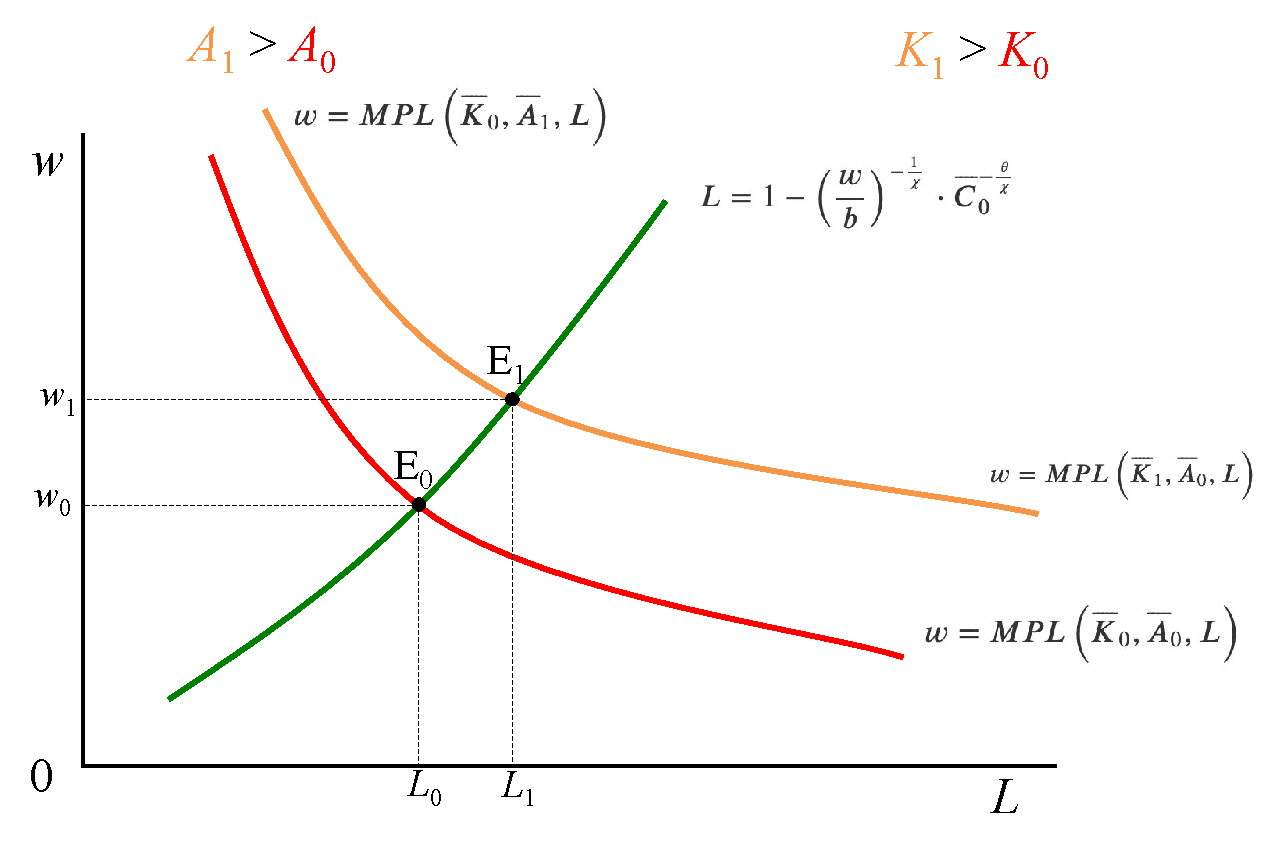
\includegraphics[width=1\linewidth]{3_0_Real_Business_Cycles/e_q_L_1.pdf}
  \caption{Case 1}
  \label{fig:sub1}
\end{subfigure}%
\begin{subfigure}{.5\textwidth}
  \centering
  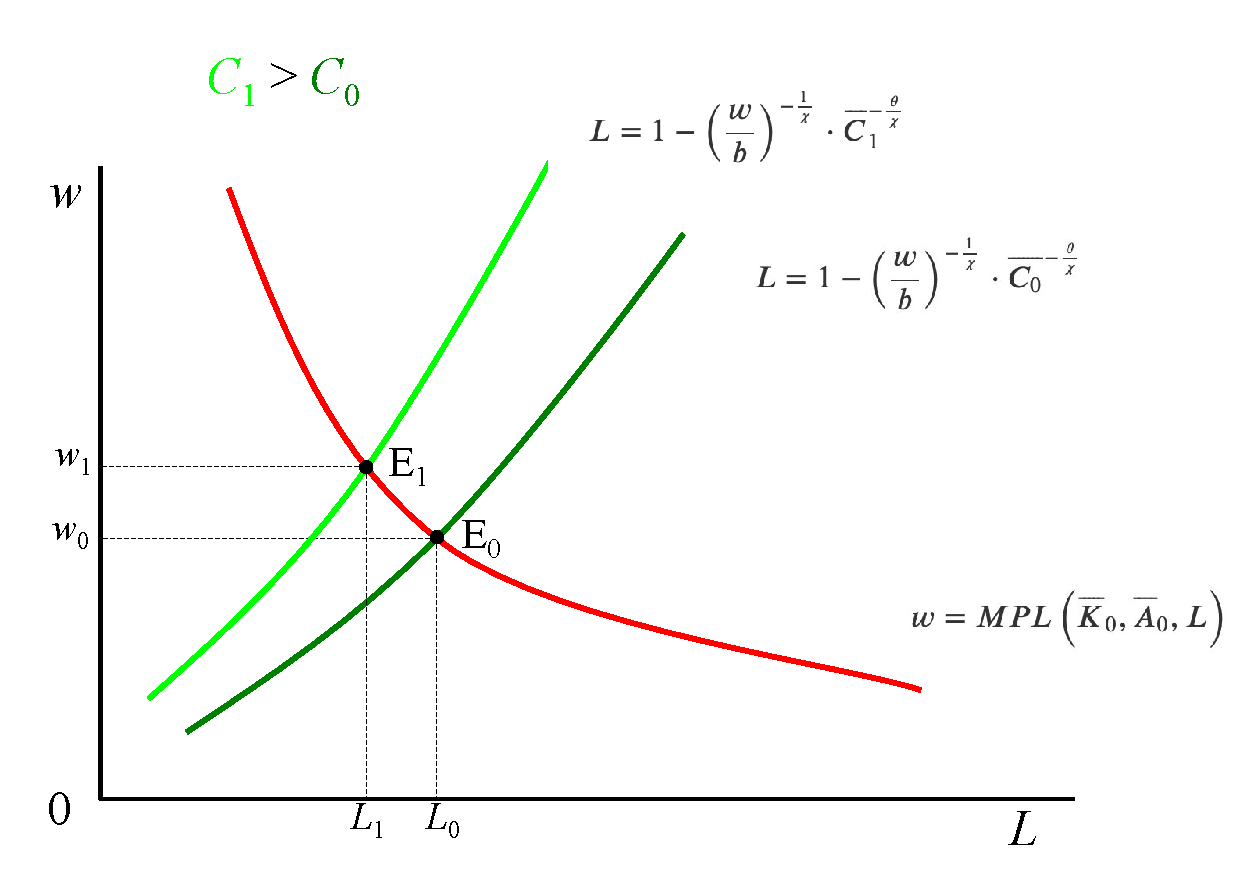
\includegraphics[width=1\linewidth]{3_0_Real_Business_Cycles/e_q_L_2.pdf}
  \caption{Case 2}
  \label{fig:sub2}
\end{subfigure}
\caption{Equilibrium in the Labour Market}
\label{fig:test}
\end{figure}

A.t S.s

\begin{equation*}
   R ^ { * } = \rho + \delta \implies  R \left( K ^ { * } , C^ { * } , A ^ { * } \right) = \rho + \delta \implies 
   \alpha \left[  \frac{A^* \cdot \mathcal{L}(K^*, C^*, A^*)}{K^*}  \right]^{1 - \alpha} = \rho + \delta
\end{equation*}

\paragraph{Steady Steady Consumption:}

$$
C^* = \mathcal{C} \left( K^*, A^*, \rho + \delta \right)
$$

$$
\frac{\partial \mathcal{C}}{\partial K} = - \frac{\frac{\partial \mathcal{R}}{\partial K}}{\frac{\mathcal{R}}{\partial C}} < 0
$$

The larger the capital stock, the larger the consumption at the steady state. 


$$
\frac{\partial \mathcal{C}}{\partial A} = - \frac{\frac{\partial \mathcal{R}}{\partial A}}{\frac{\mathcal{R}}{\partial C}} > 0
$$

Productivity is good for consumption at the steady state. 



$$
\frac{\partial \mathcal{R}}{(\rho + \delta)} = \frac{\frac{1}{\partial \mathcal{R}}}{\partial C} < 0
$$

The larger the deprecation rate, the lower the consumption at the steady state. 

There is a negative relationship

\subsection{Capital Accumulation}

$$
\Delta K_{t + 1} = WtLt + R_t K_t + \Pi_t - C_t - T_t - \delta K_t
$$

We have $\Pi = 0$ and $\Pi_t = G_t$


Output is given by: 
$$
Y = W_t L_t + R_t K_t
$$

$$
K_t^{\alpha} \cdot \left( A_t L_t \right)^{1 - \alpha} - C_t - \delta K_t - G_t
$$

Recall that $L_t$ is the labour supply function $\mathcal{L}(K_t, C_t, A_t)$

Thus we can replace to get:
$$
K_t^{\alpha} \cdot \left( A_t \cdot \mathcal{L}(K_t, C_t, A_t) \right)^{1 - \alpha} - C_t - \delta K_t - G_t
$$
We have the following derivatives of $\mathcal{L}$:

\begin{align*}
    \frac{\partial \mathcal{L} }{\partial K_t} > 0 && \frac{\partial \mathcal{L}}{\partial C_t} < 0 && \frac{\partial \mathcal{L} }{\partial A_t} > 0
\end{align*}

Long run equilibrium + dynamic

Permanent shocks:
\begin{enumerate}[a)]
    \item Productivity shocks
    \item Fiscal Policy shocks
\end{enumerate}

\newpage
\section{A prototype model: simulation and empirical validation}


\subsection{Uncertainty}

\begin{equation*}
\begin{aligned}
    \underset{C_t, L_t}{\text{max}}   E_t \Bigg\{ \sum^{\infty}_{t = \tau} \left( 1 + \rho \right)^{- (t - \tau} \cdot \left[  \frac{C_t^{1 - \theta} -1}{1 - \theta} + b \frac{(1 - L_t)^{1 - \chi} - 1}{1 - \chi} \right] \Bigg\} \\
   \text{subject to} && W_tL_t + R_tK_t - C_t - \delta K_t - T_t
\end{aligned}
\end{equation*}

Instead of maximizing utility as we did in the cases with perfect information, we now have to maximize Expected Utility $E_t$.



We need to set up a Current Value Hamiltonian (CVH), which will be:

$$
H_t = E_t \Bigg\{ \sum^{\infty}_{t = \tau} \left( 1 + \rho \right)^{- (t - \tau} \cdot \left[  \frac{C_t^{1 - \theta} -1}{1 - \theta} + b \frac{(1 - L_t)^{1 - \chi} - 1}{1 - \chi} \right] \Bigg\} + \lambda_t \left( W_tL_t + R_tK_t - C_t - \delta K_t - T_t \right)
$$

Deriving the first order conditions to solve this problem:

\begin{enumerate}[(1)]
    \item $$\frac{\partial H}{\partial C_t} \equiv \frac{\partial H}{\partial C_t} E_t \frac{C_t^{1 - \theta} - 1}{1 - \theta} - \frac{\partial H}{\partial C_t} E_t \lambda_t C_t = 0 \implies E_t C_t^{- \theta} = E_t \lambda_t $$
    
    \item $$\frac{\partial H}{\partial L_t} -b \left( 1 - L_t \right)^{ - \chi} + \lambda_t W_t = 0$$
    
        \item $$\frac{\partial H}{\partial K_t} E_t \lambda_t \cdot ( R_t - \delta ) = - E_t (\lambda_t - \lambda_{t - 1}) + \rho \lambda_{t - 1} $$

\end{enumerate}


$$
E_t \lambda_{t+1} \cdot \mathcal{R}_{t+1} = - E_t \lambda_{t+1} + (1 + \rho) \lambda_t
$$

$$
E_t (1 + \mathcal{R}_{t+1}) \lambda_{t +1} = ( 1 + \rho) \lambda_{t}
$$


$$
E_t \lambda_{t +1}^{- \theta} \cdot (1 + \mathcal{R}_{t +1}) = (1 + \rho ) \cdot C_t^{- \theta}
$$


$$
C_t^{- \theta} = \frac{1}{1 + \rho} \cdot E_t C_{t + 1}^{- \theta} \cdot (1 + \mathcal{R}_{t +1})
$$
Required assumption: Probability Distribution is stable. Why?
Correct??



\subsection{An exact solution to an approximate problem}
\paragraph{Log-Linerization of the model}
$$
X_{t+1} = f (X_t) \cdot e^{u_t}
$$

$$
\ln X_{t+1} = \ln f(X_t) + U_t
$$

$$
\ell_{t+1}
$$

$$
\Tilde{X}_{t} = \frac{X_t - X^*}{X^*} \implies \frac{X_t}{X^*} = 1 + \Tilde{X}_{t}
$$

$$
\ln \left( \frac{X_t}{X^*} \right) =  \Tilde{X}_{t}
$$

$$
\Tilde{X}_{t} = \ln X_t - \ln X^*
$$

$$
\frac{dX_t}{X^*} = d\ln X_t = \frac{(X_t^* dX_{t}) - X^*}{X^*}
$$

$$
\frac{dX_t}{X^*} \approx  \ln \left( \frac{X_t}{X^*} \right)
$$

$$
(8) \Tilde{A} = 
$$

Consumption Euler Equation on log-linear form:
$$
- \theta C^{* - \theta} \cdot \frac{\partial C_t}{C^*} = \frac{1}{1 + \rho} \left[ (1 + R)^* \cdot (- \theta) C^{* - \theta} \cdot \frac{d E_t C_{t+1}}{C^*} + C^{* - \theta} \cdot d E_t R_{t+1}   \right]
$$

Where $\frac{\partial C_t}{C^*}$ is $\Tilde{C}_t$ and $\frac{d E_t C_{t+1}}{C^*}$ is $E_t\Tilde{C}_{t+1}$

By cancelling terms and substituting our new variables we get:

\begin{equation}
- \theta \Tilde{C}_t = \frac{1}{1 + \rho} \left[ (1 + R)^* \cdot (- \theta) C^{* - \theta} \cdot E_t\Tilde{C}_{t+1} + R^*  \frac{d E_t R_{t+1}}{R^*}   \right]
\end{equation}

$R^* = \rho$

In this equation $\frac{d E_t R_{t+1}}{R^*}$ can be written as $E_t \Tilde{R}_{t+1}$

\begin{equation}\tag{$\Tilde{1}$}
    E_t\Tilde{C}_{t+1} - \Tilde{C}_t = e_1 E_t \Tilde{R}_{t + 1}
    \end{equation}
    
    $$
    e_1 = \frac{\rho}{\theta (1 + \rho )} > 0
    $$


\begin{equation}\tag{(3)}
W_t = (1 - \alpha) A_t^{1 - \alpha} \cdot \left( \frac{K_t}{L_t}  \right)^{\alpha} 
\end{equation}

\begin{equation}\tag{$\Tilde{3}$}
\Tilde{W}_t = (1 - \alpha) \Tilde{A}_t + \left( \Tilde{K_t} - \Tilde{L_t}  \right)
\end{equation}

\begin{equation}\tag{$\Tilde{6}$}
    \Tilde{Y}_t = \alpha \Tilde{K}_t + (1 - \alpha)(\Tilde{A}_t + \Tilde{L}_t)
\end{equation}

\begin{equation}
    Z_t = \left( \frac{W_t}{b} \right)^{ - \frac{1}{\chi}} \cdot C_t^{\frac{\theta}{\chi}}
\end{equation}

\begin{equation}
    Z_t 1  - L_t
\end{equation}

\begin{equation}
    \Tilde{Z}_t = - \frac{1}{\chi}\Tilde{W}_t + \frac{\theta}{\chi} \cdot \Tilde{C}_t
\end{equation}

\begin{equation}\tag{$\Tilde{2}$}
    \Tilde{L}_t = e_2 \Tilde{W}_t - e_3 \Tilde{C}_t
\end{equation}

$$
e_2 = \frac{1 - L^*}{L^*} \cdot \frac{1}{\chi} > 0
$$

$$
e_3 = \theta e_2 > 0
$$

\begin{equation}\tag{$\Tilde{4}$}
    \Tilde{R}_t = e_4 \left( \Tilde{A}_t + \Tilde{L}_t - \Tilde{K}_t  \right)
\end{equation}

$$
e_4 = \frac{\rho - \delta}{\rho}(1- \alpha) > 0
$$

\begin{equation}\tag{$\Tilde{5}$}
    \Tilde{K}_{t+1} = (1 - \delta) \Tilde{K}_t 0 e_5 \Tilde{Y}_t - e_6 \Tilde{C}_t - e_7 \Tilde{G_t}
\end{equation}

$$
e_5 = \frac{Y^*}{K^*}> 0
$$
Average product of capital, which is positive at the steady state.


$$
e_6 = e_5 \cdot \frac{C^*}{Y^*} > 0
$$

The ratio of consumption to output, or consumption divided by capital.


$$
e_7 = e_5 \cdot \frac{G^*_t}{Y^*} > 0
$$

\subsubsection*{Solving the dynamic model}


$$
E_t \Tilde{K}_{t +1} = \Tilde{K}_{t + 1}
$$

$$
E_t \Tilde{A}_{t + 1}= 
$$
\begin{equation}\label{matrix_solution}
\begingroup % keep the change local
\renewcommand*{\arraystretch}{2}
\begin{bmatrix}
E_t \Tilde{C}_{t +1} \\
\Tilde{K}_{t +1} 
\end{bmatrix}
=
\begin{bmatrix}
a_{1,1} & a_{1,2} \\
a_{2,1} & a_{2,2} 
\end{bmatrix}
\begin{bmatrix}
\Tilde{C}_t \\
\Tilde{K}_{t} 
\end{bmatrix}
+
\begin{bmatrix}
b_{1,1} & b_{1,2} \\
b_{2,1} & b_{2,2} 
\end{bmatrix}
\begin{bmatrix}
\Tilde{A}_t \\
\Tilde{G}_{t} 
\end{bmatrix}
\endgroup
\end{equation}


Fill in eigenvalues Candidate Solution


Laws of motion


$$
\tilde { c } _ { t } = a _ { CK} \cdot \tilde { k } _ { t } + a_ { CA } \cdot \tilde { A } _ { t } + a _ { CG } \cdot \tilde { G } _ { t }
$$

$$
\Tilde{K}_{t + 1} = b_{KK} \cdot \Tilde{K}_t + b_{KA} \cdot \Tilde{A}_t + b_{KG} \cdot \Tilde{G}_t
$$

From \ref{matrix_solution} we have:

$$
E_t \Tilde{C}_{t +1} = a_{CK} \cdot \Tilde{K}_{t + 1} + a_{CA} \cdot E_t \Tilde{A}_{t + 1} + a_{CG} \cdot E_t \Tilde{G}_{t + 1}
$$


$$
b _ { K G  } = a _ { 21 } \cdot a _ { CG } + b _ { 22 }
$$

$$
b _ { KA } = a _ { 2 1 } \cdot a _ { C A } + b _ { 21 }
$$


$$
b _ { KK } = a _ { 21 } a _ { CK } + a _ { 22 }
$$




\subsection{Empirical Validation}

\subsubsection{Calibration}

\subsection{Comparing the RBC model with data}

\paragraph{Pros}
\begin{enumerate}[(a)]
    \item Consumption is less volatile than output
    \item Investment is volatile than output ???
    \item Capital stock is much less volatile than output
    \item Real wages and the average product of labour are procyclical, as expected
    \item Employment is procyclical
    \item Time series created by the model is similar to data
\end{enumerate}

\paragraph{Cons}
\begin{enumerate}[(a)]
    \item Average product of labour is more procyclical than what is shown by data
    \item A positive correlation between employment and APL, but in reality the correlation is negative. 
    \item 

\end{enumerate}

\newpage
\chapter{The New Keynesian School}


\section{Predecessors: Walrasian and non-Walrasian equilibria}


\subsection{Non-walrasian equilibrium models}

Spillover effects

\begin{equation*}
\begin{aligned}
& \underset{C, L}{\max}
& & U = C ^ { \alpha } ( 1 - L ) ^ { 1 - \alpha } \\
& \text{s.t}
& & P \cdot C \leq W \cdot L + \pi
\end{aligned}
\end{equation*}


\begin{equation*}
    \mathcal{L} = C ^ { \alpha } ( 1 - L ) ^ { 1 - \alpha } + \lambda(P \cdot C \leq W \cdot L + \pi)
\end{equation*}



$$
\text{MRS}_{Z, c} = \frac{w}{p}
$$

$$
\frac{1 - \alpha}{\alpha} \cdot \frac{C}{1 - L}
$$


The notional consumption function (unrestricted):
\begin{equation}
    \Tilde{C} = \alpha \frac { W \cdot 1 + \pi } { P }
\end{equation}


Notional labour supply:
\begin{equation}
    \Tilde{L} = 1 - ( 1 - \alpha ) \frac { W \cdot 1 + \pi } { W }
\end{equation}


An additional constraint where:
$$
L \leq \Bar{L}_0
$$

\begin{equation}
    L ^ { * } = \min \left\{ \overline { L } _ { 0 } , \Tilde{L} \right\}
\end{equation}

\begin{equation}
    C ^ { * } = \min \left\{ \overline { Y } _ { 0 } , \Tilde{C} \right\} = \left\{ \alpha \frac { W \cdot \overline { L } _ { 0 }  + \pi } { P }, ... \right\}
\end{equation}

\subsubsection*{Microeconomic Foundations}
\paragraph{Assumptions}
\begin{enumerate}
    \item No rationed agents on both sides of the market
    \item Rationing scheme is non-manipulable
    \item Markets are perfectly competitive
\end{enumerate}

\subsubsection*{Partial equilibrium}
Partial equilibrium exists in the minimum of notional supply and demand, look at the slides

\subsubsection*{General Equilibrium}

$$
P = \left[ P_1, P_2, \dots, P_n  \right]
$$

$$
\mathbf{X} = \Downarrow (P)
$$

$$
\mathbf{X^*} = \Downarrow X (\mathbf{P, \overline{Z}})
$$

\subsection*{An Illustrative Model}

\subsubsection*{Assumptions}
\begin{enumerate}
    \item $n = 1$ --- Number of goods in the economy
    \item $\alpha = 1$ --- Labour does not give any disutility
    \item $\Phi = 0$ --- No fixed costs
    \item $\Psi = 0$ --- No costs to change prices  - Menu Costs
    \item $M = \infty$ --- Number of firms producing each good
    \item $A = 1$
    \item Population = 1
\end{enumerate}

\subsubsection*{The Household Problem}

\begin{equation*}
\begin{aligned}
& \underset{C, M}{\max}
& & U = C ^{\gamma} \cdot \frac{M}{P}^{1 - \gamma} \\
& \text{s.t}
& & M_E + wL + \pi -T = M + PC \\
& & &  L  = \min \left\{ \overline { N }  , 1 \right\}
\end{aligned}
\end{equation*}

Since Labour does not gives any disutility, households wants to work as much as possible. If $\Bar{N} < 1$ the household is rationed in the labour market and can only work less than what they want. 


The demand for consumption goods:

\begin{equation}
    C = \gamma \frac{M_E + wL + \pi -T}{P}
\end{equation}

The notional demand for consumption is given by the following equation, when $L = 1$:

\begin{equation}
   \Tilde{C} = \gamma \frac{M_E + w \cdot 1 + \pi -T}{P}
\end{equation}


The effective demand is given by the following expression, which is the minimum between the notional demand for consumption goods and the case where $L = \Bar{N}$:
\begin{multline}
    \Tilde{C} = \min \left\{ \Tilde{C}, \gamma \frac{M_E + w \overline{N} 1 + \pi -T}{P} \right\} = \\
      \gamma \left( \frac{M_E - T}{P} + Y^* \right) \implies \\
     \gamma \frac{M_E}{P} + \gamma \left( Y^* - \frac{T}{P} \right)
\end{multline}

Where $\gamma$ represents the marginal propensity to consume.


\subsubsection*{Government}
As opposed to households, the government can never be rationed

$$
\Tilde{G} = G^* = \overline{G}
$$


The total demand is given by Household consumption $C^*$ plus Government Consumption $G^*$
$$
D^* = C^* + G^* = \gamma \left( \frac{M_E - T}{P} + Y^* \right) + \overline{G}
$$

\[ Y^* = \left\{ \begin{array}{ll}
         f(1) & \mbox{if $L^* = 1$};\\
        f(\overline{N}) & \mbox{if $L^* = \overline{N}$}.\end{array} \right. \] 
        
        
        
$$
L^* = \min \left\{ \overline{N}, 1 \right\}
$$

\subsubsection*{Firms}

\begin{equation*}
\begin{aligned}
& \underset{\Pi}{\max}
& & \Pi = PY - WN \\
& \text{s.t}
& & Y = 1N^\beta \\
& & &  Y \leq D \\
& &  & N \leq 1
\end{aligned}
\end{equation*}

$$
TC = WN = W \cdot Y^{\frac{1}{\beta}}
$$

$$
MC  = \frac{1}{\beta} W \cdot Y^{\frac{1 - \beta}{\beta}}
$$

$$
P = MC
$$

The notional supply of goods
$$
\Tilde{Y} = \left( \frac { P \cdot \beta} { W } \right) ^ { \frac { \beta } { 1 - \beta } }
$$

Notional demand for labour
$$
\Tilde{N} = \left( \frac { W } { \beta \cdot P } \right) ^ { \frac { 1 } { 1 - \beta } }
$$

\subsubsection*{If the firm is rationed in the goods market: }

$$
\Tilde{Y} > \overline{D} = Y^*
$$

Which means that we have excess supply ?


$$
1 N^{\beta} = \overline{D} \implies N = \left( \frac{D}{1} \right)^{\frac{1}{\beta}} 
$$


Effective Labour Demand
$$
N^* = \min \left\{ \left( \frac { W } { \beta \cdot P } \right) ^ { \frac { 1 } { 1 - \beta } },  \left( \frac{D}{1} \right)^{\frac{1}{\beta}}   \right\}
$$

\subsubsection*{If the firm is rationed in the labour market: }

$$
\Tilde{N} > \Tilde{L} = 1 = L^*
$$


$$
Y = 1(N^*)^\beta = 1
$$

Effective labour Supply
$$
Y^* = \min \left\{ \left( \frac { P \cdot \beta} { W } \right) ^ { \frac { \beta } { 1 - \beta } }, 1   \right\}
$$

Check slides for more regimes

\subsection*{Keynesian Unemployment Regime}
The Keynesian regime exhibits excess supply in both markets.
$$
P > P_w
$$

$$
\frac{W}{P} > \left( \frac{W}{P} \right)_W
$$

$$
D^* = \gamma \left( \frac{M_E - T}{P} + Y^* \right) + \overline{G}
$$

$$
N^* = D^{* \frac{1}{\beta}} < \Tilde{L} = 1
$$

\begin{align}
    Y^* = D^* \implies \\
    &  Y^* = \gamma \left( \frac{M_E - T}{P}  \right) + -  \gamma Y^* \overline{G} \implies \\
\end{align}

Autonomous demand is given by:
$$
\Omega \equiv \gamma \frac{M_E - T}{P} + \overline{G}
$$

So we have: 

$$
Y^* = \frac{\Omega}{1 - \gamma}
$$

$$
N* = \left( \frac{\Omega}{1 - \gamma}  \right)^{\frac{1}{\beta}} < 1
$$

$$
\frac{\partial Y^*}{\partial G^*} = \frac{1}{1 - \gamma} > 1
$$

$$
\frac{\partial Y^*}{\partial M_E} = \frac{\gamma}{(1 - \gamma) P} > 0
$$

\clearpage

\subsection*{Classical Unemployment Regime}
With classical unemployment we have excess supply of labor and an excess demand for goods. 

$$
N^* = \Tilde{N} = \left( \frac { W } { \beta \cdot P } \right) ^  { - \frac { 1 } { 1 - \beta }} < \Tilde{L} = 1
$$
\begin{equation}\label{YStar}
    Y^* = 1 \cdot N^{*\beta} = \left(  \frac{w}{\beta P} \right)^{ - \frac{1}{1 - \beta}} 
\end{equation}

We can rewrite the previous equation as a function of real wage instead of nominal wage by defining $\omega$;
$$
\omega \equiv \frac{w}{P}
$$

Thus from \ref{YStar} we have: 
$$
\left( \frac{\omega}{\beta} \right) ^{ - \frac{\beta}{1 - \beta}}
$$




\paragraph{Policies}

\begin{align*}
    \frac { \partial Y ^ { * } } { \partial \overline { G } } = 0 && \frac { \partial Y ^ { * } } { \partial M_E } = 0 
    &  & \frac{\partial Y^*}{\partial \omega} = - \frac{Y^*}{1 - \beta} * \frac{\beta}{\omega} < 0
\end{align*}

By looking at the partial derivatives we see that government consumption through $\overline{G}$ is ineffective and will not change the level of unemployment, the same goes for monetary policy through $M_E$. Firms are already selling as much as they want at the given prices. The problem is that the prices is not???

There is excess demand in the economy and therefore Keynesian demand stimulating policies would not work. 

However, the only thing that would work is price and income policies to affect the real wage. This is clear by looking at the $\tfrac{\partial Y^*}{\partial \omega}$ which is negative. This means that if you could reduce the real wage production could be stimulated because they are too high. Examples of such policies could be labour market regulations and so on.  Such policies would not work in a Keynesian regime as the real wage do not affect output. 



\subsubsection*{Suppressed Inflation}
In the suppressed inflation unemployment regime we have excess demand in both markets; 

$$
\Tilde{L} < \Tilde{N} \land \Tilde{Y} < \Tilde{D}
$$
$$
\Tilde{N} > \Tilde{L} = 1 \implies L^* = 1
$$

$$
Y^* = 1 \cdot N^{* \beta} = 1
$$

$$
Y^* = C^* + \overline{G} \implies C^* = 1 - \overline{G}
$$

\clearpage


\paragraph{Putting everything together --- Delimitation of the regimes}
\begin{table}[ht]
\begin{tabu} to \linewidth{|X[-2.5,c,m]|X[c,m]|X[c,m]|}
\tabucline-
    \backslashbox{Labour Market}{Product Market} & $$\Tilde{Y} > \Tilde{D}$$ & $$\Tilde{Y} < \Tilde{D}$$  \\ \hline
    $$\Tilde{L} > \Tilde{N}$$  & Keynesian Unemployment & Classical Unemployment \\ \hline
    $$\Tilde{L} < \Tilde{N}$$ & Not possible due to the absence of stockage & Suppressed Inflation   \\ \hline
\end{tabu}
\caption{Unemployment regimes}
\end{table}

\begin{figure}[h!]
    \centering
    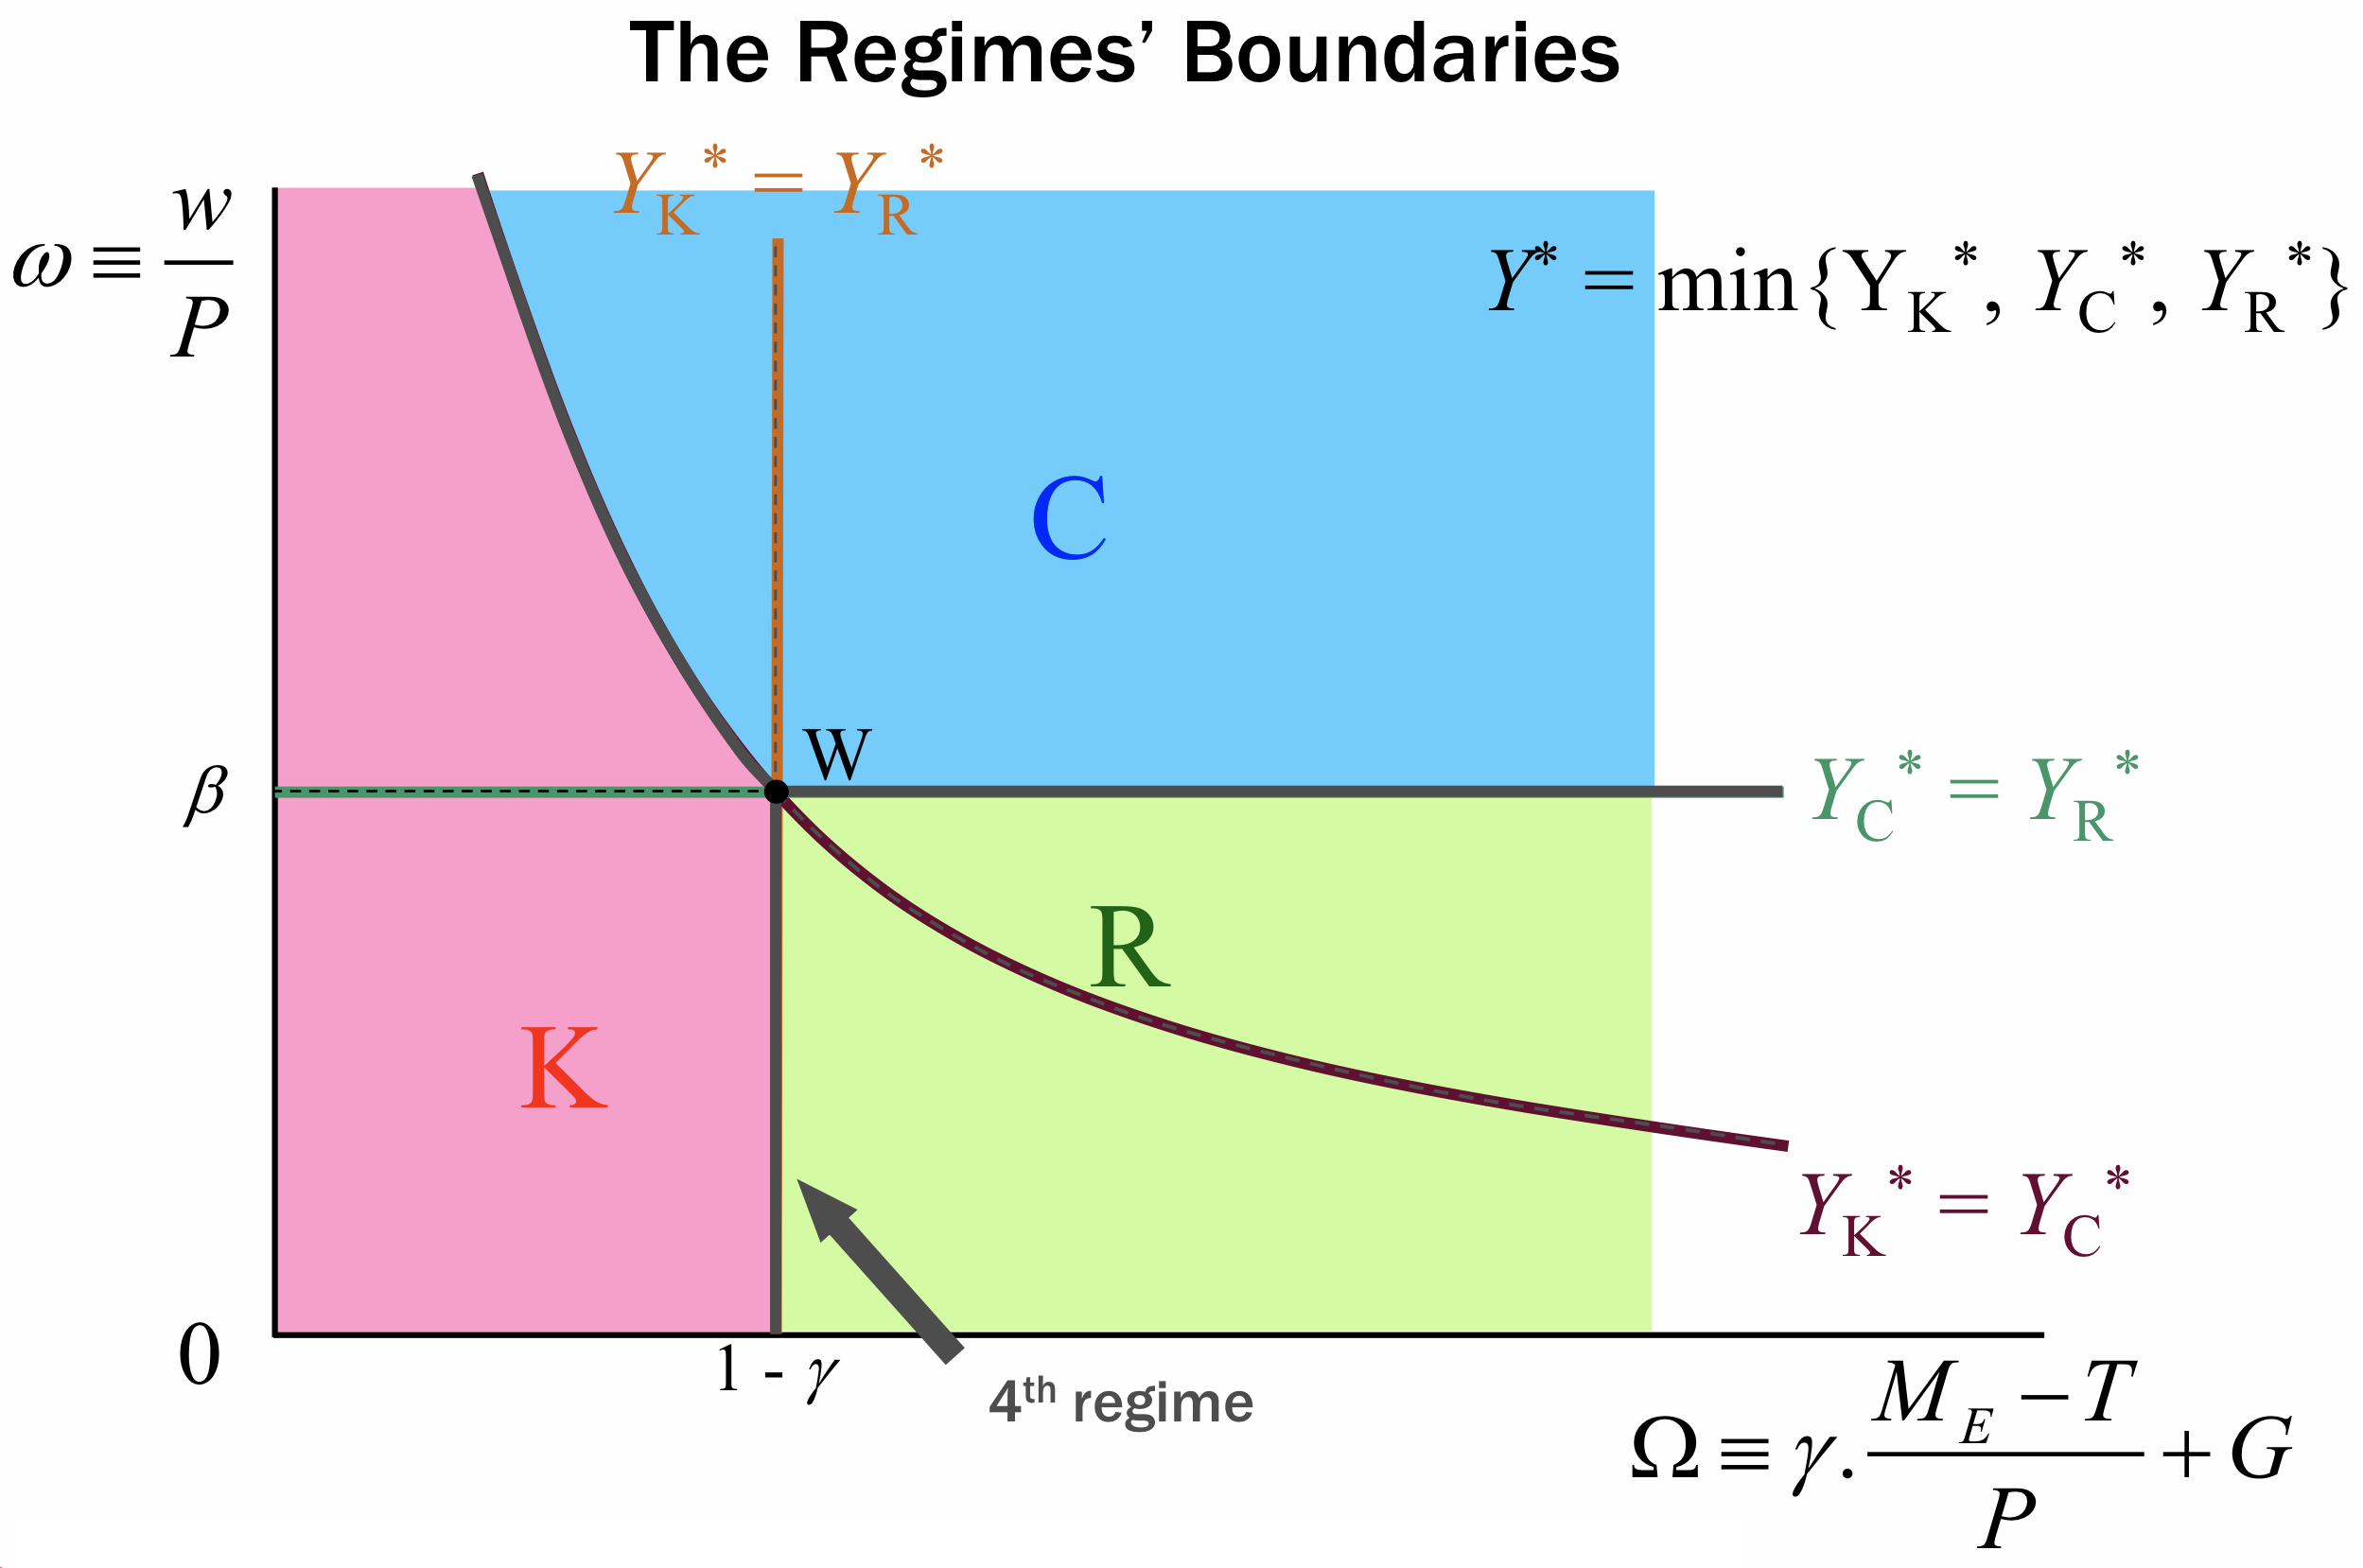
\includegraphics[width=\textwidth]{4_0_New_Keynesian_School/regime_boundaries.png}
    \caption{Regime Boundaries}
    \label{fig:my_label}
\end{figure}
\clearpage

\newpage
\section{Imperfect competition in the Goods Market}



\subsection*{Consequences of imperfect competition in partial equilibrium}


\subsubsection{Firms}

Firm $i$ competes with other firms in the same industry, using quantity as their strategic variable to determined the price. This is known as \textit{Intra-industrial Cournot Competition}. In addition, they take the average price level as given. 

Firm $i$ produces good $j$ and has the following profit function $\Pi_i (j)$
\begin{equation*}
    \Pi_i(j) = p ( j ) \cdot  y _ { i }(j) - \text{TC}_i(j)
\end{equation*}

The condition to maximizing profits under imperfect competition is given by:
$$
MR_i = MC_i 
$$
 Maximizing profits yields:
 $$
 MC_i (y_i) = p(j)\left( 1 + \frac{1}{\epsilon_i(j)} \right)
 $$
 
 
 The Price Elasticity is given by:
 $$
 \epsilon_i (j) = \frac{\partial Y}{\partial p(j)} \cdot \frac{p(j)}{Y_i} < 0 
 $$
Which is negative 

\paragraph{}
 Marginal Revenue for a firm under imperfect competition is always below the price. We know that a firm under perfect competition is a price taker. Under imperfect competition, the firm knows that if they want to sell more they have to reduce the price, depending on the price elasticity. The expression and result of the elasticity depends on the market structure. 
 
 If we assume that labour is the only input, the profit function will be given by:

 $$
 \Pi_i = p(j)\left[\underbrace{A_i \cdot f(N_i - \Phi)}_\mathbf{{Y_i}}   \right] A_i (N_i - \Phi) - wN_i
 $$
 
 

 Where $\Phi$ is fixed administrative costs, $N_i$ is the labour required by the firm and $A_i$ is productivity of labour. 
 
 $$
 \text{MPL}_i (N_i - \Phi ) \left( 1 + \frac{1}{\epsilon_i (j)} \right) = \frac{w}{p(j)}
 $$
 
  Under perfect competition the marginal product of labour should be equal to the wage, but this is not the case under imperfect competition, where we also need to consider the elasticity.
 Imperfect competition in the gods market also has spillover effects into the labour market, because lower production leads to lower labour demand. There is no involuntary unemployment, because the wage rate is lower and people would not want to work as much. Imperfect competition in the goods market is not enough to generate unemployment, however, it will generate underemployment compared to the perfect competition equilibrium. 
 
 
 \subsection{A Simple General Equilibrium Model with Imperfect Competition compared with Non-Walrasian equlibrium}
 
 \subsubsection{Assumptions}
 \begin{itemize}
     \item $U_m = \emptyset$ --- No Utility of Money, meaning that fiscal policy is the only thing that is important. 
     \item $M_E = 0$ --- No money endowment
     \item $m = 1$ --- The continuum of goods. All industries are the same, with one producer in each industry. Number of producers in a given industry, ie. we have monopolistic competition where firms compete on prices in a Bertrand like situation with slightly differentiated products. Every producer is a monopolist, but the goods are substitutes in some manner.  
     \item $\beta  = 1 $
     \item $A_i = 1$ --- Constant technology/productivity to simplify
     \item $\Psi = 0$ --- No Menu Costs
\end{itemize}

\subsubsection{Households}


Households are deciding between consumption and leisure
\begin{equation*}
\begin{aligned}
& \underset{C, Z}{\max}
& & U(C,Z) \\
& \text{s.t}
& & wL + \Pi -T = \int_{0}^{n} p(j) \cdot c(j) \cdot dj \\
& & & Z = 1 - L \\
& & & T = T_0 + t(wL + \Pi) \\
& & & C = \left[ n^{\frac{\lambda - 1}{\sigma}} \cdot \int_{0}^{n} c(j)^{\frac{\sigma - 1}{\sigma}} \cdot dj   \right]^\frac{\sigma}{\sigma - 1}
\end{aligned}
\end{equation*}

Where $\lambda \in \left[0,1 \right]$, and represents the love for variety. If $\lambda = 0$ you are indifferent between the different goods, with a $\lambda > 0$ you get more utility of consuming a more varied set of goods. 

\subsection*{1st step}
With homothetic preferences we can use the constraint to rearrange:
$$
wL + \Pi - T = PC
$$

Where $P$ is the price index and $C$ is the consumption index. Thus $PC$ can be seen as a cost-of-living index. 

Then we can substitute the tax function:
$$
wL + \Pi - T_0 + t(wL + \Pi) = PC
$$

Dividing by $P$ and solving for $C$ yields:
$$
C = \frac{w(1-t)}{P}L_t + \frac{\Pi(1-t)-T_0}{P}
$$

Where $\frac{w(1-t)}{p}L_t$ is the labour-income which we define as $\omega_N$ and $\frac{\Pi(1-t)-}{p}$ is the non-labour income (dividends etc.) that does not depend on labour, which we define as $\Theta_N$. Thus consumption can be written as:

$$
C = \Theta_N + \omega_N \cdot L 
$$


The consumption decision is therefore a function of the real wage and non-labour income. 
$$
C \equiv \mathcal{C}\left(\omega_N, \Theta_N \right)
$$

Given that leisure and the consumption good are normal goods. We have the following partial derivatives:

\begin{align*}
    \frac{\partial \mathcal{C}}{\partial \omega_N} > 0 && \frac{\partial \mathcal{C}}{\partial \Theta_N} > 0
\end{align*}

An increase in the real wage increases consumption, the same for an increase in non-labour income. 



The labour decision is a function of the real wage and non-labour income. 
$$
L \equiv \mathcal{L}\left(\omega_N, \Theta_N  \right)
$$

\begin{align*}
    \frac{\partial \mathcal{L}}{\partial \omega_N} > 0  && \frac{\partial \mathcal{C}}{\partial \Theta_N} < 0
\end{align*}

An increase in the real wage has two effects on the labour supply, but we can't say for sure which effect is stronger: 
\begin{itemize}
    \item When the wage rate goes up, leisure is more expensive and you want less leisure because of the substitution effect. 
    \item With a higher wage rate, you can have more income and you want to work more. 
\end{itemize}

An increase in non-labour income leads to a lower labour supply. 

\subsection*{2nd Step --- Finding the optimal inflation}

\begin{equation*}
\begin{aligned}
& \underset{c_j}{\min}
& & \int _ { 0 } ^ { n } p(j) \cdot c(j) \cdot dj \\
& \text{s.t}
& & C = n^\frac{1 - \lambda}{1 - \sigma}  \left[\int _ { 0 } ^ { n } c(j)^\frac{\sigma - 1}{\sigma} dj     \right]^\frac{\sigma}{\sigma - 1} 
\end{aligned}
\end{equation*}

The demand function for good $j$
$$
c(j) = \left[ \frac{p(j)}{P}  \right]^ - \sigma \cdot \frac{C}{n^{1 - \lambda}}
$$

The demand function consists of two parts:
\begin{itemize}
    \item If $\lambda = 0$, if all prices are the same, the consumption of good $j$ will just be just dividing the number of baskets by the number of goods. 
    \item If the good is more expensive the average good, you want to consume less of good $j$ and more of the other goods.
\end{itemize}


The price index $P$ is given by:
$$
P = \left[\frac{1}{n^{1 - \lambda}} \int_0^n p(j)^{1 - \sigma} dj  \right]^\frac{1}{1 - \sigma}
$$

\subsubsection{Government}

$$
T = \int _ { 0 } ^ { n } p ( j ) \cdot y ( j ) \cdot d j
$$


Government has a similar demand to the consumers for the goods in the economy:
$$
G = h ^ { \frac { 1 - \lambda } { 1 - \sigma } } \left[ \int _ { 0 } ^ { n } g ( j ) d \right) ] ^ { \frac { \sigma - 1 } { \sigma } }
$$


Which can be written as:

$$
g(j) = \left[ \frac{p(j)}{p} \right]^\sigma \cdot \frac{G}{n^{1-\lambda}}
$$


\subsubsection{Firms}

Total production of good $j$ --- which is only produced by firm $i$:

$$
Y(j) = c(j) + g(j) = \left[  \frac{p(j)}{P}  \right]^{-\sigma} \cdot \frac{D}{n^{1-\lambda}}
$$

Where $D$ is the total of private and government consumption, in other words; aggreagate demand:
$$D \equiv C + G$$

Because we are under monopolistic competition, $D$ is both the market demand in industry $j$ and the demand function faced by each individual firm. In another market structure, such as oligopoly, the Demand would be shared between the firms. 

In monopolistic competition will be given for each firm, so the individual firm can take $D$ as given, the same goes for $\mathbf{P}$ and the mass of the continuum of goods; $\overline{n}$. The firm can use this assumption because it is very small compared to the economy as a whole. For instance, an increase in the individual price would not be able to affect the price index $\mathbf{P}$


The profit maximization problem for the firm is now:
\begin{equation*}
\begin{aligned}
& \underset{}{\max}
& & \Pi(j) = p(j) \cdot y(j) - wN(j) \\
& \text{s.t}
& & p(j) = \mathbf{P} \left[ \frac{y(j) n^{1-\lambda}}{D} \right]^{ - \frac{1}{\sigma}} \\
& & & y(j) + \Phi = \underset{\mathbf{A}}{1} \cdot N(j)
\end{aligned}
\end{equation*}


Given the first order condition for profit maximization in imperfectly competitive markets:
$$
\text{FOC: } MR = MC
$$

We get:
$$
p ( j ) \cdot \left[ 1 + \frac { 1 } { \epsilon ( p ) } \right] = \underbrace{MC \left[ y(j) \right]}_{\frac{w}{A} = N}
$$

$$
\epsilon_i (j) = - \frac{\sigma}{v(j) \cdot s_ij}
$$

$$
V(j) = \frac{y(j)}{\frac{D}{n}}
$$

Where $V(j)$ expresses an industry production compared to the average industry, thus if $V(j) > 1 $ we are producing more than the average and $V(j) < 1 $ we are producing less than the average.  

$$
S_i (j) = \frac{y_i(j)}{Y(j)}
$$

$S_i$ expresses the production of firm $i$ that produces $j$ divided by the production in the industry, thus $S_i$ is a firms share in an industry. If all firms are equal in each industry and we have $m$ firms the $S_i$ equation is simply:

$$
\frac{1}{m}
$$

Since we are talking about monopolistic competition this is simply 1. Intra industrial symmetrical eq???


\paragraph{Lerner Index:}

$$
\mu(j) = \frac{p(j) - MC(j) }{p(j)} \in \left[ 0,1 \right]
$$

The Lerner Index is a measure of a firms market power in a given industry. A larger $\mu$ implies a stronger market power of firm $j$.

In our case $\mu = 1/\sigma$, which we get by substituting the expression for $p(j)$ and since we only have labour $MC = w$

\subsubsection*{Macroeconomic Variables}

In any macroeconomic model we need ... . Imagine that you have $n$ goods in an economy. How many prices would you have? $n - 1$ prices, because you have to express the absolute prices of all the goods in terms of another good. Since we don't have money in this economy we have to chose a good to act as the \textit{numeraire}. Under perfect competition any good can be the numeraire, however, in imperfect competition it is not as straightforward as it can change the outcome as the results. In this case we chose the price of the consumption basket $\mathbf{P}$ as our numeraire. The $\mathbf{P}$ is defined as:

$$
\mathbf{P} = \left[  \frac{1}{n^{1-\lambda}} \cdot \int_0^n p(j)^{1-\sigma} \cdot dj \right]^\frac{1}{1 - \sigma}
$$

We can simplify this into: 
$$
\mathbf{P} = \left[  \frac{1}{n^{1-\lambda}} \cdot n\cdot p^{1-\sigma}  \right]^\frac{1}{1 - \sigma} \implies n^{- \frac{\lambda}{\sigma - 1} }p
$$

If all the firms are the same, the average price is not equal to the individual price, unless there is no love for variety. 

Value added GDP:
$$
Y = \int_{0}^{n} \frac{p(j) y(j)}{\mathbf{P}}dj
$$

Because $\mathbf{P = 1}$ and we know $p(j)$ and all firms are identical so we can calculate 

$$
n^{1 + \frac{\lambda}{\sigma - 1}} \cdot y(j)
$$

If there is market clearing in each industry then:
$$
Y(j) = c(j) + g(j) \implies C + G
$$

Love for variety....



Profits



$$
\pi \int _ { 0 } ^ { n } \pi ( j ) d j = n \left[p(j) y(j) - wN(j) \right]
\implies
np(j)y(j) - nw\left( y(j) + + \Phi \right)
$$

Real profits $\tfrac{\pi}{P}$, but since $P = 1$:

$$
\pi = \mu \cdot y - n^{1 + \frac{\lambda}{\sigma - 1}} \cdot ( 1 - \mu) \Phi
$$

Ignoring fixed costs $\Phi = 0$ and $\mu = 0$:

$$
Y \implies = 0
$$

To get perfect competition, you need constant returns to scale as well as $\mu = 0$



Labour Market:
$$
L = \int_0^n N(j) dj \implies \int_0^n \left[y(j) + \Phi \right]dj
$$

\paragraph{A General Formulation of the equilibrium}
$$
Y = C + G = Y = \mathcal{C} \left(\omega_N, \Theta_N \right) + G
$$

$$
\omega_N \equiv \frac{w}{P}(1-t) \implies (1-t)n^{\frac{\lambda}{\sigma - 1}} (1-\mu)
$$

$$
\Theta_N \equiv \frac{\pi(1-t) - T_0}{\mathbf{P}} = (1-t)\left[ \mu y - n^{\frac{1 + \lambda}{\sigma - 1}} \cdot (1 - \mu) \Phi \right] - T_0
$$

Inefficiency results from imperfect competition:
\begin{itemize}
    \item Welfare is lower in imperfect competition
    \item Consumption is lower
    \item Output i slower
    \item Employment is lower. 
\end{itemize}


The equilibrium values are given by the following equations. Where they are functions of different values, but in this case we are focusing on $G$. 

\begin{align*}
    w^* = w(G,...) && \pi^* = \pi(G,...) && t^* = t(G,...) && T_0 = T_0(G,...)
\end{align*}

$$
Y^* = \mathcal{C} \left[w^*(1-t^*), \pi^*(1-t^*) - T_0 \right] + G
$$


$$
Y^* = w^*L^* + \pi^* 
$$


\begin{tcolorbox}[fontupper=\large, fontlower=\normalsize]
\subsubsection{Fiscal Policy Effectivness}
\begin{equation}\label{fiscal_policy_effectivness}
dY^* = \mathcal{C}^*_{\omega_N} \left[(1-t)dw^* - w^* dt^* \right] + \mathcal{C}^*_{\Theta_N}\left[(1-t)d\pi^* - \pi^* dt^* - dT_0 \right] +dG
\end{equation}
\tcblower
To derive the value of the output government-consumption multiplier, $m^* = \frac{dY^*}{dG}$
\end{tcolorbox}


\begin{align*}
    \frac{\partial \mathcal{C}}{\partial \omega_N} \equiv \mathcal{C}^*_{\omega_N}
&& \frac{\partial \mathcal{C}}{\partial \Theta_N} \equiv \mathcal{C}^*_{\Theta_N}
\end{align*}

In the initial equilibrium there are no pure profits, thus $\pi = 0$ so equilibrium output is only dependent on labour income


\paragraph{Case 1: Government Controls $t$ and $G$}
In this case the government controls both the marginal tax rate and public expenditure. By looking at the government budget constraint, you will see that the lump sum tax becomes endogenous because we have no deficits: $T_0 = G - tY^*$


$$
dt^* = 0 \implies dT^*_0 = dG - t \cdot \frac{\partial Y^*}{\partial G}
$$

Which you can replace in \ref{fiscal_policy_effectivness}.

\paragraph{Case 2: No Lump Sum Taxes and Government controls $G$}


$$
t^* = \frac{G}{Y^*}
$$


$$
dT_0 = 0 \implies dt^* = \frac{dGY^* - \frac{\partial Y^*}{G}dG \cdot G}{(Y^*)^2} \implies \left( 1 - \frac{\partial Y^*}{G} \cdot \frac{G}{Y^*} \right) \cdot \frac{dG}{Y^*}
$$





\subsection{The initiators: Dixon(1987) and Mankiw(1988)}

Recall equation \ref{fiscal_policy_effectivness} where we now define $\mathcal{C}^*_{\omega_N}$ and $\mathcal{C}^*_{\Theta_N}$ as $\alpha$ for simplificiation purposes. 
Two similar models. 

Assumptions

Assuming a Cobb-Douglas Utility function:


\begin{align*}
    U = C^\alpha Z^{1-\alpha} && 0 < \alpha < 1
\end{align*}

Consumption is given by:

\begin{equation}\label{consumption}
    C = \alpha \left( w _ { N } + \Theta _ { N } \right)
\end{equation}



Labour supply is given by:
$$
L = 1 - ( 1- \alpha) \frac{\omega_N + \Theta_N}{\omega_N}
$$

Where $\alpha$ can be seen as the marginal propensity to consume for both labour and non-labour income. 


A few asumptions:


Since we only have have lump sum taxes:

$$
t^* = 0 \implies dt^* = 0
$$

The marginal tax rate is zero and it does not change. 

No Love for variety: 

$$
\lambda = 0
$$


The mass continuum of the goods is fixed, and it does not change:
$$
n = \overline{n} \implies dn^* = 0
$$

Output in equilibrium:

$$
Y^* = \alpha \left( w^* \cdot 1 - \pi^* - T^*_0 \right) + G
$$

The real wage and the aggregate price index is given by:
\begin{align*}
    w^* = 1 - \mu
    &&
    \mathbf{P} = 1
\end{align*}


Profits are:
$$
\pi = \mu Y^* - \overline{n}(1-\mu) \cdot \Phi
$$

Ricardian economy with no deficit budgets and any increase in government needs to be finaned with increased taxes:
$$
T_0 = G
$$


Solving the model:

\begin{equation*}
    Y^* = \frac{\alpha (1- \mu) \cdot (1- \overline{n} \Phi)}{1 - \alpha \mu} + \frac{1 - \alpha}{1 - \alpha \mu}G
\end{equation*}

\begin{equation*}
    dy^*=\mathcal{C}_{\omega N}^* \bigg[(1-t^*)dw^* - w^*dt^* \bigg] + \mathcal{C}_{\Theta N} \bigg[ (1-t)d\pi^*-\pi^*dt^*-dT_{0}^*\bigg] + dG      
\end{equation*}

$$
 \left. \frac{\partial Y^*}{\partial G} \right\rvert_{dT^*_0 = dG} = \frac{1 - \alpha}{1 - \alpha \mu} > 0
 $$
 
 Which is the fiscal multiplier $m^*$, which is positive, thus fiscal policy is effective even with a balanced-budget multiplier. 
 

Deriving the multiplier. First look at the derivatives of \ref{consumption} with respect to net real wage and non-labour income:

\begin{align*}
    \frac{\partial C}{\partial \omega_N} = \alpha && \frac{\partial C}{\partial \Theta_N} = \alpha
\end{align*}

We can rewrite \ref{fiscal_policy_effectivness} given the above and the following results depending on the response to shocks in fiscal policy:

\begin{itemize}
    \item Marginal tax rate is zero --- $t = 0$
    \item The wage rate does not respond to fiscal policy shocks --- $dw = 0$
    \item We are financing with lump sum taxes --- $dt = 0$
\end{itemize}

 $$
 dY^* = \alpha \left[ (1 - 0 ) \cdot 0 - (1 - \alpha) \emptyset \right] +
 \alpha \left[ (1 - \emptyset) \cdot \mu \frac{\partial Y^*}{\partial G} \cdot dG - dG  \right] + dG
 $$
 
One important mechanism is the effect of fiscal policy on profits
 
 The only way you get a 1-to-1 fiscal policy multiplier you need $\mu = 1$

 $$
 dY^* = ( 1 - \alpha) dG + \alpha \mu \frac{\partial y^*}{\partial G} \cdot dG
 $$
 $$
 ( 1- \alpha \mu) \frac{\partial Y}{\partial G} = ( 1 - \alpha ) \implies 
 $$
 
$$
 \left. \frac{\partial Y^*}{\partial G} \right\rvert_{dT^*_0 = dG} = \frac{1 - \alpha}{1 - \alpha \mu} 
$$
 
\begin{equation}\tag{$m^*_A$}
     \frac{\partial k_A^*}{\partial \mu} = \frac{\alpha (1 - \alpha)}{( 1 - \alpha )^2} > 0
\end{equation}
 
 
\subsection{Distortionary Taxation: \textcite{molana_note_1992}}
This model is taken from \citetitle{molana_note_1992} by \textcite{molana_note_1992}


$$
T_0 = 0 \implies dT_0^* = 0
$$

$$
t^*Y^* = G \implies t^* = \frac{G}{Y^*}
$$

$$
\frac { \partial Y ^ { * } } { \partial G } = \frac{Y^* - \alpha(1-\mu)}{Y* \left[ 1 - \alpha (1 - t^*) \mu  \right]}
$$


$$
Y^* = C^* \implies C^* = \alpha ( 1- t^*)(1 - \mu + \pi^*)
$$

Since we have zero profits and only lump sum taxes both  $t^* = 0 $ and $\pi^* = 0$ the above equation is simply:
$$
C^* = \alpha \left( 1 - \mu  \right)
$$

The conclusion is that fiscal policy is totally ineffective. 


\subsection{Free Entry: \textcite{startz_monopolistic_1989}}
This model is taken from \citetitle{startz_monopolistic_1989} by \textcite{startz_monopolistic_1989}

$$
n^* = \pi(n^*) = 0 \implies n^* = \frac{\mu Y^*}{(1 - \mu) \Phi}
$$

So the fiscal policy multiplier is:
\begin{equation}\tag{$m^*_C$}
 \left. k^*_c = \frac{\partial Y^*}{\partial G} \right\rvert_{dT^*_0 = dG, \frac{d\Pi^*}{dG} = 0 } = 1 - \alpha
\end{equation}

$$
C = \frac{W + \Pi  - T}{1 + a^\epsilon \cdot w^{1 - \epsilon}}
$$


$$
\mathcal{C}^*_{\Theta_L} = \frac{1}{1 + a^\epsilon \cdot w^{1 - \epsilon}}
$$

Where
$$
w^* = 1 - \mu
$$

The $\epsilon$ elasticity is important. The way for $\mu$ to affect the marginal propensity is if $\epsilon$ is different from one, if $\epsilon = 1$ we get a Cobb-Douglas. 

$$
\frac{\partial \mathcal{C}^*_{\Theta_L}}{\partial \mu}
$$

\subsection{Preferences: Dixon and Lawler}

 - Startz assumptions + $U=u(C,Z)$


Rewriting \ref{fiscal_policy_effectivness} gives:

\begin{equation*}
    dy^*=\mathcal{C}_{\omega N}^*\bigg[(1-t^*)\cdot 0-(1-\mu)\cdot 0\bigg] + \mathcal{C}_{\Theta N}^*\bigg[(1-0)\cdot 0-dG\bigg]+dG
\end{equation*}


So the fiscal policy multiplier is:
\begin{equation}\tag{$m^*_D1$}
    \left. k^*_{D1} = \frac{\partial Y^*}{\partial G} \right\rvert_{dT^*_0 = dG, \frac{d\Pi^*}{dG} = 0 } = 1 - \mathcal{C}_{\Theta N} \in [0,1]
\end{equation}

\begin{equation*}
    \frac{\partial k^*_{D1}}{\partial \mu}=\frac{\partial \mathcal{C}_{\Theta N}}{\partial \mu}=-(\epsilon -1 )\frac{(1-\mu)^{-\epsilon}\cdot a^\epsilon}{\big[ 1+a^\epsilon+(1-\mu)^{1-\epsilon}\big]^2} 
\end{equation*}

\begin{align*}
    u=\big(C^{\frac{\epsilon -1 }{\epsilon}}+aZ^{\frac{\epsilon-1}{\epsilon}}\big)^{\frac{\epsilon}{\epsilon -1}} && a>0 && \epsilon \geq 0
\end{align*}

\begin{align*}
    C=\frac{w+\pi-T}{1+a^{\epsilon}w^{1-\epsilon}} && \mathcal{C}_{\Theta N}^*=\frac{1}{1+a^\epsilon w^{* 1-\epsilon}} && w^*=1-\mu
\end{align*}

There are three scenarios: 
\begin{enumerate}
    \item If $\epsilon=1$, and the utility function is a Cobb-Douglas, you'll get the Startz result; 
    \item If $\epsilon>1 \implies \frac{\partial k^*_{D1}}{\partial \mu}<0$
    \item If $\epsilon<1 \implies \frac{\partial k^*_{D1}}{\partial \mu}>0$ 
\end{enumerate}

\subsection{Effects on Wages}

The income effect is always the same. 

Elasticity of substitution ($\epsilon$) will make the substitution effect, either big ($\epsilon>1$) or small ($\epsilon<1$)
\subsubsection{Lover for Variety}

$$
0 < \lambda \leq 1
$$
\subsubsection{ Devereux et \& al. (1996) - Increasing returns to specialization}
$$
y = \bigg[ n^{\frac{\lambda-1}{\sigma}} \int_0^n y(j)^\frac{\sigma-1}{\sigma}dj   \bigg]^\frac{\sigma}{\sigma - 1}
$$

With a positive $\lambda$:
$$
\Pi^* = 0 \implies n^*=\bigg[\frac{\mu y^*}{(1-\mu)\Phi}\bigg]^{\frac{1}{1+\frac{\lambda}{\sigma-1}}}
$$

$$
w^*=n^{*\frac{\lambda}{\sigma-1}}(1-\mu)
$$

$$
\frac{\partial w}{\partial G}=\frac{\lambda}{\lambda + \sigma -1}\frac{w^*}{y^*}\frac{\partial y^*}{\partial G}=\frac{\lambda}{\lambda+\sigma-1}\frac{1-(1-\alpha)\frac{G}{y^*}}{\alpha}\frac{\partial y^*}{\partial G}
$$

\begin{equation}\tag{$m^*_e1$}
k^*_{e1}=\frac{\partial y^*}{\partial G}\bigg\rvert_{dT^*_0=dG,G=0,\frac{d \pi^*}{\d G=0}}=(1-\alpha)\bigg(+\frac{\lambda n}{1-\mu} \bigg)
\end{equation}


$$
\frac{\partial k^*_{e1}}{\partial \mu}=(1-\alpha)\frac{\lambda}{(1+\mu)^2}>0
$$

Which is positive. 

$$
y^*=w^*L^*+\pi^*=(1-\mu)n^{*\frac{\lambda}{\sigma-1}}L^*
$$


\subsubsection{Endogenous Markups: \cite{costa_endogenous_2004}}
This model is taken from \citetitle{costa_endogenous_2004} by \textcite{costa_endogenous_2004}


\begin{enumerate}
    \item $ \lambda = 0$
    \item $n = \overline{n}$
    \item $m \leq 1$ 
\end{enumerate}


$$
\pi^* = \mu^*Y^* - \overline{n}m^* \cdot w^*  \cdot \Phi^*
$$


$$
w^*= 1 - \mu*
$$

$$
m = \frac{1}{\sigma \cdot \mu^*}
$$

$$
\Pi = 0 \implies \mu^* = \frac{\phi^*}{1 + \phi^*}
$$

Where $\phi$ is an increasing returns to scale indicator:

$$
\phi^* = \frac{\overline{n} \Phi m^*}{Y^*}
$$

$$
\Pi = 0 \implies \sigma \mu^{*^2} \cdot Y^* + n \Phi\mu^* - \overline{n}\Phi = 0
$$

$$
2\sigma\mu^* + \sigma\mu^{*2}dY^*+n\Phi d\mu^*=0
$$

$$
\frac{d\mu^*}{dY^*}=\frac{\sigma\mu^{*2}}{2\sigma\mu^*Y^*+\overline{n}\Phi}<0
$$

$$
-\frac{\sigma\mu^{*3}}{n\Phi(2-\mu^*)}
$$


$$
y^*=\frac{\overline{n}\Phi(1-\mu^*)}{\sigma\mu^*}
$$


\begin{equation}\tag{$m^*_e2$}
k_{e2}=\frac{\partial y^*}{\partial G}\bigg\rvert_{dt_{0}=dG, \frac{d \pi^*}{dG}=0}=\frac{1-\alpha}{1-\frac{\sigma\mu^{*3}}{\overline{n}\Phi(2-\mu^*)}}
\end{equation}






\newpage
\section{Nominal Rigidity}


\subsection{Menu Costs}




    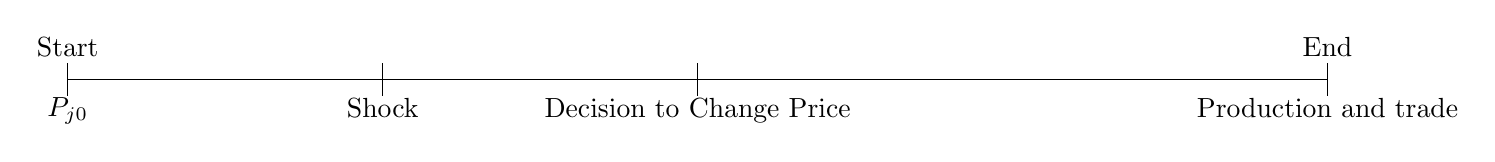
\begin{tikzpicture}[scale=2]
     % draw horizontal line   

      \draw (0,0) -- (8,0);



      % draw vertical lines
       \foreach \x in {0,2,4,8}
       \draw (\x cm,3pt) -- (\x cm,-3pt);

        % draw nodes
       \draw (0,0) node[below=3pt] {$P_{j0}$ } node[above=5pt] {Start};
       \draw (2,0) node[below=3pt] {Shock};
       \draw (4,0) node[below=3pt] {Decision to Change Price};
       \draw (8,0) node[below=3pt] {Production and trade} node[above=5pt] {End};

       \end{tikzpicture}
       
       
\paragraph{Partial Equilibrium analysis}
\begin{itemize}
    \item Monopolistic Competition
    \item Macroeconomic variables:
        \begin{itemize}
        \item $\overline{D}$ --- Demand is given
            \item $\mathbf{P} = \mathbf{\overline{P}}$ --- Prices are fixed and equal to the price index
            \item $n = \overline{n}$ --- The mass of contiuum of goods is fixed
        \end{itemize}
\end{itemize}

Demand for firm $j$ is given by:

$$
Y_j = Y_j\left(p_j ,D  \right) \implies p_j = p_j \left( Y_j, D  \right)
$$

Where 

\begin{align*}
    \frac{\partial Y}{\partial p_j} < 0 && \frac{\partial Y}{\partial D} > 0
\end{align*}

Meaning that the output for firm $j$ is decreasing in price and increasing in demand.

\paragraph{Choosing the initial price}

$$
\overline{D} = \overline{D}_0
$$

$$
w = \overline{w}_0
$$

$$
p_j \left( y_j, \overline{D}_0 \right) - \left( 1 - \frac{1}{\sigma_j}  \right) = MC(y_j) 
$$

2 Conditions for this period:
\begin{align*}
    \overline{D} = \overline{D} && w = \overline{w}
\end{align*}

Which means that the firm takes both the demand and wage as given. 

\paragraph{Changing the prices}

\begin{align*}
    p_{j1}^* = p_j \left( Y_{j1}^*, \overline{D}_1 \right) \\
    &&& p_{j1}^* =
\end{align*}

$$
TC_j = wf^{-'} \left(  \frac{y_j}{A_j}  \right)
$$

\subsubsection{Aggregate Demand Expansion}
$$\Delta \pi _ { j } = \pi_j - \pi^*_j = (D - A) + \Psi p$$

Price change iff:

$$\Delta \pi_j > 0 \implies \mathbf{P} \Psi > A - D$$

If the change in profit is positive, meaning that the menu cost is smaller than the gain in profit.


$$
\Delta CS = A + B > 0
$$

$$
\Delta SW = \Delta CS + \Delta \pi _ { j } = A + B + (D - A) + \Psi \implies
D + B + \mathbf{P} \Psi > 0
$$



\subsubsection{Aggregate Demand Contraction}

$$
\pi^*_{j1} - \pi_{j1} = (H - E) - \Psi \mathbf{P}
$$

A firm would keep their price unchanged iff:

$$
\Delta \pi < 0 \implies \mathbf{P} \Psi > H- E
$$

$$
\Delta CS  = E + F
$$

$$
\Delta SW = - \left(  \Delta CS + \Delta \pi_j  \right) \implies (E + F) + (H - E) - \Psi \mathbf{P} \implies F + H - \mathbf{P} \Psi
$$

From a social point of view it is preferable to keep prices unchanged iff the menu costs are larger than F + H, thus very large menu costs. Such large menu costs are not likely and we would not expect that the social optimum is to keep the prices unchanged. However, from the point of the view of the firm  

\subsubsection{General Equlibrum Model}

\paragraph{Assumptions}
\begin{enumerate}
    \item No Government: $G = T = 0$
    \item $M_E = \overline{M_E}$ --- Money endownment is fixed
    \item $A_j = 1$
    \item $B = 1$
    \item $\Phi = 0$ --- No fixed administrative costs
\end{enumerate}

Assumption 4 and 5 together tells us that we have Constant Returns to Scale in this case. 

\paragraph{Households}

$$
C = \gamma \alpha \frac { \overline { M _ { E } } + w + \pi } { \mathbf { P } }
$$

$$
M= ( 1 - \gamma) \left( \overline { M _ { E } } + w + \pi \right)
$$

$$
L = 1 - \gamma \left( 1 - \alpha  \right) \frac{\overline{M_E} + w + \pi}{w}
$$

Initial EQ:

$$
p_j \left(1 - \frac{1}{\sigma}  \right)  = w (MC)
$$

$$
\pi_j = p_j y_j - wN_j = \left( p_j - w  \right)y_j \implies \frac{p_j y_j}{\sigma}
$$

$$
\mathbf{P} = p_j
$$

$$
\pi = \frac{p y}{\sigma}
$$

$$
w = \mathbf{P} \frac{\sigma - 1}{\sigma}
$$

$$
C = ....
$$

$$
Y = C
$$

$$
Y = 1 \cdot N
$$

$$
N = L
$$

$$
L = ... insert
$$

$$
w = \mathbf{P} \frac{\sigma - 1}{\sigma}
$$

$$
\pi = \frac{p y}{\sigma}
$$

$$
M = ...
$$


\begin{align}
    Y = C \implies \\
    Y = \gamma \alpha \frac { \overline { M _ { E } } + w + \pi } { \mathbf { P } } \implies \\
    \overline{M_E} + w + \pi = \frac{p y}{\gamma \alpha}
\end{align}

\begin{align}
    Y = L \implies \\
    Y = L = 1 - \gamma \left( 1 - \alpha  \right) \frac{\overline{M_E} + w + \pi}{w} \implies \\
    Y_0^* = \frac{\alpha ( \sigma - 1 )}{\sigma - \alpha}
\end{align}


\begin{align}
    M_E + w + \pi = \frac{p y}{\gamma \alpha} \implies \\
    \mathbf{P_0^*} = \frac{\gamma (\sigma - \alpha}{(\sigma - 1)(1 - \gamma)}\overline{M_E}_0
\end{align}


Assumption:

$$
\overline{M_E}_0 = \frac{(\sigma - 1)(1 - \gamma)}{\gamma (\sigma - \alpha)} \implies \mathbf{P_0^*} = 1
$$

\paragraph{Monetary Shock with menu Costs}

$$
\mathbf{P} = \overline{\mathbf{P_0}} = 1
$$

$$
\pi = py - wN
$$


$$
Y = C ...
$$

\begin{align}
    Y = L \implies \\
    Y = 1 - \gamma \left( 1 - \alpha  \right) \frac{Y}{ \gamma \alpha w} \implies \\
    w = \frac{1 - \alpha}{\alpha} \cdot \frac{Y}{1 - Y}
\end{align}



$$
\pi = (1 - w)Y
$$

$$
\pi + w = ...... = \frac{Y}{\alpha}
$$


$$
Y = \gamma \alpha \left( \overline{M_E} + \frac{Y}{\alpha}     \right) \implies \\
Y = \frac{\gamma \alpha}{1 - \gamma}\overline{M_E} \implies \\
Y_1 = k \overline{M_E}
$$

Where $k$ is:

$$
k = \frac{\gamma \alpha}{1 - \gamma} > 0
$$


$$
 \left. \frac{\partial Y^*}{\partial \overline{M_E}} \right\rvert_{k} = \frac{\gamma}{(1 - \gamma)\mathbf{\overline{P_0^*}}}
 $$
 
 \paragraph{Welfare}
 
 $$
 U = \left[ C^{\alpha} (1-L)^{1-\alpha}   \right]^{\alpha} \cdot \left( \frac{M}{P}    \right)^{1 - \gamma}
 $$
 
 
 $$
 \Tilde{U} = \gamma \left[  \alpha \Tilde{C} + (1 - \alpha)\Tilde{Z}   \right] + (1 - \gamma)(\Tilde{M} - \mathbf{\Tilde{P}})
 $$

$$
L^* = Y^* \implies \Tilde{L} = \Tilde{Y}
$$

$$
Z = 1 - L \implies \Tilde{Z} = - \frac{dL}{1 - L_0^*} = \frac{Y_0^*}{1 - Y_0^*}\Tilde{Y}
$$


$$
\Tilde{U} = 
\left \{
\gamma \left[ \alpha - (1 - \alpha) \cdot \frac{\alpha (\sigma -1)}{\sigma (1 - \alpha)} + (1 - \gamma)  \right] M_E
\right \}
$$

In the above equation we have the following:
\begin{itemize}
    \item  The $\alpha$ co-responds to the change in consumption $\Delta C$
    \item Change in Liquidity Services + Real Money Balances
    \item Change in leisure, because output goes up people would have to work more which reduces Leisure. 
\end{itemize}

By simplifying you can arrive at:

$$
\Tilde{U} = \frac{\sigma (1 - \gamma)+\alpha \gamma}{\sigma} \overline{M_E}
$$

Welfare multiplier $V > 0$ Why?


$$
\mu_{Actual} = \frac{\mathbf{P} - w}{\mathbf{P}} = 1 - w \implies
1 - \frac {1 - \alpha } { \alpha } \cdot \frac { Y } { 1 - y }
$$

$$
d\mu_{Actual} = - \frac{1- \alpha}{\alpha} \cdot \frac{dY}{(1 - Y_0^*)^2}
$$

\paragraph{Notes on alternative 2 in GE}

$$
Y_j = \left( \frac{P_j}{\mathbf{P}}  \right)^{- \sigma} \left( \frac{C}{n} + \Psi   \right)
$$

$$
VA_j = \frac{p_j}{\mathbf{P}}Y_j - n\Psi \implies \sum_{j} VA_j = nY_j  - n \Psi
$$


$$
Y_1^* = 1 N - n \psi 
$$




$$
\pi_j^* = \mathbf{P}(Y + n \Psi) - wN - n\mathbf{P}\Psi = \mathbf{P}Y - w\Tilde{N}
$$



\subsubsection{Primary conclusions of the Menu Costs}
\begin{enumerate}[i]
  \item The existence of menu costs can lead to much larger losses in welfare, than the cost to the individual firm.
  \item Asymmetric incentives for firms: Adjustment is better with demand expansion, but worse with demand contractions.
  \item Menu costs are a short run market friction, in the long-run price will adjust to its natural level.
\end{enumerate}


\newpage
\subsection*{Time Dependent Models}
\subsection{A Particular Case: Calvo Pricing}

Exogenous decision on price changes, done by a random lottery. The lottery defines who can change prices, and who can't, not necessarily the actual changes in prices that ensue.  


\paragraph{}

\begin{figure}[ht]

\centering
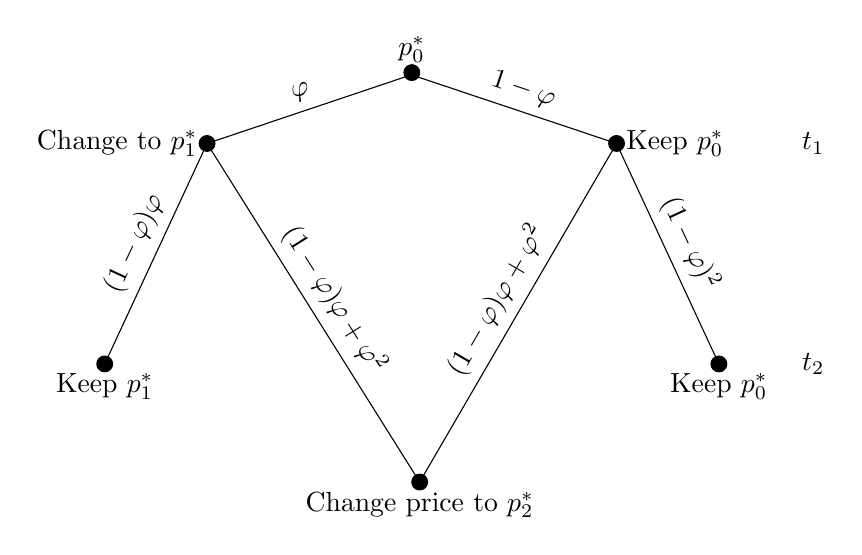
\begin{tikzpicture}[scale=1]


\coordinate (a) at (3.83, 2.65);
\coordinate (c) at (1.3, 1.8);
\coordinate (d) at (4, -2.5);
\coordinate (e) at (0,-1);
\coordinate (f) at (7.8, -1);




\draw [fill] (c) circle [radius=0.1] node [left] {Change to $p_1^*$};
\draw [fill] (6.5, 1.8) circle [radius=0.1] node [right] {Keep $p_0^*$};
\draw [fill = black] (3.9, 2.7) circle [radius=0.1] node [above] {$p_0^*$};
\draw [fill] (d) circle [radius=0.1] node [below] {Change price to $p_2^*$};
\draw [fill] (e) circle [radius=0.1] node [below] {Keep $p_1^*$};
\draw [fill] (f) circle [radius=0.1] node [below] {Keep $p_0^*$};


\draw (e)-- (c) node[pos=0.5,sloped,above] {$(1-\varphi)\varphi$};
\draw (a) -- (c) node[pos=0.5,sloped,above] {$\varphi$}; 




\draw (3.96, 2.65) -- (6.5, 1.8) node[pos=0.5,sloped,above] {$1-\varphi$};
\draw (6.5, 1.8) -- (7.8, -1) node[pos=0.5,sloped,above] {$(1-\varphi)^2$};
\node at  (9, 1.8) {$t_1$};
\node at  (9, -1) {$t_2$};


\draw (c) -- (d) node[pos=0.5,sloped,above] {$(1-\varphi)\varphi+\varphi^2$};
\draw (6.5, 1.8) -- (d) node[pos=0.5,sloped,above] {$(1-\varphi)\varphi+\varphi^2$};


\end{tikzpicture}
\caption{Decision tree}
\end{figure}

In the first period each firm has a probability $\varphi$ do be able to change prices, and a probability $(1- \varphi)$ that they can't.
In the second period: 
\begin{itemize}
    \item there is a probability $(1-\varphi)^2$ that companies that didn't change prices in the last period can't change prices again;
    \item a probability $(1-\varphi)\varphi$ that companies who changed prices last period can't change prices in this one;
    \item a probability $(1-\varphi)\varphi+\varphi^2$ that companies who either kept the last prices, or changed it in the last period, can change prices in this period;
\end{itemize}

And it goes like this for every period, until the last one where: 
\begin{itemize}
    \item $(1-\varphi)^{\tau}$ companies will have kept the first price $p^{*}_{0}$;
    \item $(1-\varphi)^{\tau -1}\varphi$ will have kept $p^{*}_{1}$;
    \item $(1-\varphi)^{\tau - 2}\varphi^2$ will have kept $p^{*}_{2}$;
    \item And so on.
\end{itemize}

If $\varphi =1$, companies can always choose to change prices, and the condition for their price comes as: 
\begin{equation*}
    p^{*}_{j\tau}.(1+\frac{1}{\varepsilon_{j\tau}})=MC_{j\tau}
\end{equation*}
This means that companies will always be changing prices to adjust to their marginal cost, and the elasticities they face, if they need to. 

\paragraph{}
\subsubsection{Micro Foundations}
The problem of the firm comes, in this situation, as: 

\begin{equation*}
    \underset{p_{j\tau}}{max} E_{t}\sum_{\tau=t}^{\infty}(1+\rho)^{-(\tau-t)}.(1-\varphi)^{\tau-t}.\pi(p_{j\tau})
\end{equation*}

Where 
\begin{equation*}
\begin{aligned}
\pi(p_{j\tau})=p_{j\tau}.y_{j\tau}-w_{\tau}.N_{j\tau} \\
\pi(p_{j\tau})=p_{j\tau}(\frac{p_{j\tau}}{P})^{-\sigma}D_{t}-w_{\tau}\frac{y_{j\tau}}{A_{\tau}} \\
\pi(p_{j\tau})=P_{\tau}^{\sigma}D_{\tau}-(p_{j\tau}^{1-\sigma}.\frac{w_{\tau}}{A_{\tau}}.p_{j\tau}^{-\sigma})
\end{aligned}
\end{equation*}
Note that $y_{j\tau}$ is the same as $y_{j}$ in the last section. Also $\frac{w_{\tau}}{A_{\tau}}$ is the Marginal Cost at period $\tau$.

Substituting in the maximization problem, comes:

\begin{equation}
     \underset{p_{j\tau}}{max} \sum_{\tau=t}^{\infty}(\frac{1-\varphi}{1+\rho})^{\tau-t}E_{t}[P_{\tau}^{\sigma}D_{\tau}-(p_{j\tau}^{1-\sigma}.\frac{w_{\tau}}{A_{\tau}}.p_{j\tau}^{-\sigma})]
\end{equation}

Let's call the equation being maximized, $V_{t}$.

\begin{equation*}
    \frac{\partial V_{t}}{\partial p_{j\tau}}=0 \\
    \implies \sum_{\tau=t}^{\infty}(\frac{1-\varphi}{1+\rho})^{\tau-t}.E_{t}\frac{\partial \pi_{j\tau}}{\partial p_{j\tau}}=0
\end{equation*}

\begin{equation*}
\begin{aligned}
    E_{t}\frac{\partial \pi_{j\tau}}{\partial p_{j\tau}}=E_{t}[(1-\sigma)P_{\tau}^{\sigma}D_{\tau}p_{j\tau}^{-\sigma}+\sigma\frac{w_{\tau}}{P_{\tau}}P_{\tau}D_{\tau}p_{j\tau}^{-(-\sigma-1)}] \\
    E_{t}\frac{\partial \pi_{j\tau}}{\partial p_{j\tau}}=(\sigma-1)E_{t}[P_{\tau}D_{\tau}.p_{j\tau}^{-(\sigma-1)}(p_{j\tau}^{*}-p_{j\tau}] \\
    \text{Where,} && p_{j\tau}^{*}=\frac{\sigma}{\sigma-1}\frac{w_{\tau}}{A_{\tau}}
\end{aligned}
\end{equation*}

In the Steady State: 
\begin{equation*}
    p_{j\tau}^{*}=p^{*} \implies y_{j\tau}^{*}=(\frac{p^{*}}{P^{*}})^{-\sigma}.\frac{D^{*}}{n=1} \implies y_{j\tau}^{*}=D^{*}
\end{equation*}
    
\begin{equation*}
\begin{aligned}
    dE_{t}X_{\tau}(p_{j\tau}^{*}-p_{j\tau})=E_{t}(p^{*}-p^{*})dX_{\tau}+X^{*}(dp_{j\tau}^{*}-dp_{j\tau}) \\
    \text{Where,} && X_{\tau}=P_{\tau}^{\sigma}D_{\tau}p_{j\tau}^{-\sigma-1} \\
    E_{t}[P^{*\sigma}D^{*}p^{*(-\sigma-1)}(dp_{j\tau}^{*}-dp_{j\tau})]E_{t}[D^{*}(\Tilde{p_{j\tau}^{*}}-\Tilde{p}_{j\tau})]=D^{*}E_{t}[\Tilde{p}_{j\tau}^{*}-p_{j\tau}]
\end{aligned}
\end{equation*}

From here we take the optimal pricing rule in the Calvo Model:

\begin{equation}
    \sum^{\infty}_{\tau=t}(\frac{1-\varphi}{1+\rho})^{\tau-t}E_{t}(\Tilde{p_{j\tau}^{*}}-\Tilde{p_{j\tau}})\simeq 0 
\end{equation}

Note that $p_{j\tau}=p_{j\tau}^{*}(1+\Tilde{p}_{j\tau})$

\begin{equation*}
   \begin{aligned}
    \sum^{\infty}_{\tau=t}(\frac{1-\varphi}{1+\rho})^{\tau-t}\Tilde{p}_{j\tau}=\sum^{\infty}_{\tau=t}(\frac{1-\varphi}{1+\rho})^{\tau-t}E_{t}p_{j\tau}^{*} \\ \text{Where,} && \Tilde{p}_{j\tau}=\Tilde{p}_{jt} \\
    \Tilde{p}_{jt}\sum^{\infty}_{\tau=t}(\frac{1-\varphi}{1+\rho})^{\tau-t}=\Tilde{p}_{jt}\frac{1}{1-\frac{1-\varphi}{1+\rho}} \\
    \Tilde{p}_{jt}\frac{\varphi+\rho}{1+\rho}=\sum^{\infty}_{\tau=t}(\frac{1-\varphi}{1+\rho})^{\tau-t}E_{t}p_{jt}^{*} \\ 
   \implies \Tilde{p}_{jt}=\sum^{\infty}_{\tau=t}\varpi_{\tau-t}E_{t}\Tilde{p}_{j\tau}^{*}
   \end{aligned}
\end{equation*}
$\varpi_{\tau-t}$ comes as:
\begin{equation*}
       \varpi_{\tau-t}=\frac{\varphi+\rho}{1+\rho}(\frac{1-\varphi}{1+\rho})^{\tau-t} 
\end{equation*}

And follows the condition:
\begin{equation*}
        \sum^{\infty}_{\tau=t}\varpi_{\tau-t}=1
\end{equation*}

To finish defining the micro variables in the model: 
\begin{equation*}
    \begin{aligned}
        p_{j\tau}=\frac{\sigma}{\sigma-1}.MgC_{j\tau} \\
        \Tilde{p}_{j\tau}=\Tilde{MgC}_{j\tau} \\
        \Tilde{MgC}_{j\tau}=\rho_{MgC}\Tilde{MgC}_{j,\tau-1}+\varepsilon_{MgC,\tau}
    \end{aligned}
\end{equation*}
Note the Marginal Cost is determined by an AR(1) process.

\subsubsection{Aggregate Dynamics}
Assume a fixed number of companies $n_{t}=\overline{n}$.
In the Steady State, $p_{j\tau}=p^{*}$, and $P_{t}^{*}=p_{t}^{*}$.

\begin{equation*}
    P_{t}=(\frac{1}{n}\sum^{\overline{n}}_{j=1}p_{jt}^{1-\sigma})^{\frac{1}{1-\sigma}}
\end{equation*}

\begin{equation*}
      dP_{t}=\frac{1}{1-\sigma}(\frac{1}{n}\sum^{\overline{n}}_{j=1}p^{*(1-\sigma)})^{\frac{1}{1-\sigma}-1}(1-\sigma)\frac{1}{n}\sum^{\overline{n}}_{j=1}p^{*-\sigma}dp_{jt} 
\end{equation*}

\begin{equation*}
\begin{aligned}
    dP_{t}=\frac{1}{\overline{n}}\sum^{\overline{n}}_{j=1}dp_{jt} \\
    \Tilde{P}_{t}=\frac{1}{\overline{n}}\sum^{\overline{n}}_{j=1}\Tilde{p}_{jt}
\end{aligned}
\end{equation*}

The number of companies that set a price different from that of the last period is given by $\varphi.\overline{n}$. With the old prices there are $(1-\varphi)\overline{n}$.

\paragraph{}
Let's see the aggregate price levels in different periods. Starting with $t=1$:

\begin{equation*}
    \Tilde{P}_{1}=\frac{1}{\overline{n}}[\varphi.\overline{n}+(1+\varphi)\overline{n}.\Tilde{p}_{0}]=\varphi\Tilde{p}_{1}+(1+\varphi)\Tilde{p}_{o}=\varphi\Tilde{p}_{1}
\end{equation*}
Because $\Tilde{p}_{0}=0$.
For $t=2$:
\begin{equation*}
    \Tilde{P}_{2}=\frac{1}{\overline{n}}[\varphi\overline{n}.\Tilde{p}_{1}+(1-\varphi)\overline{n}.\Tilde{p}_{0}]=\varphi\Tilde{p}_{2}+(1+\varphi)\Tilde{P}_{1}
\end{equation*}
By the same rationale, we can generalize for any period t, 
\begin{equation} \label{Price_aggregate_Calvo}
\begin{aligned}
    \Tilde{P}_{t}=\varphi\Tilde{p}_{t}+(1-\varphi)\Tilde{P}_{t-1} \\
    \Tilde{P}_{t}=\varphi\sum^{\infty}_{\tau=t}\varpi_{\tau-t}E_{t}\Tilde{P}_{t}^{*}+(1+\varphi)\Tilde{P}_{t-1}
\end{aligned}
\end{equation}

We can now look at the evolution of inflation $\pi_{t}$

\begin{equation*}
    \pi_{t}=\frac{P_{t}}{P_{t-1}}-1 \implies 1+\pi_{t}=\frac{P_{t}}{P_{t-1}}
\end{equation*}

Translating this to the notation on our model, 
\begin{equation*}
    \pi_{t}=\Tilde{P}_{t}-\Tilde{P}_{t-1}=\varphi\big(\sum^{\infty}_{\tau=t}\varpi_{\tau-t}E_{t}P_{\tau}^{*}-\Tilde{P}_{t-1}\big)
\end{equation*}

\subsubsection{Inflation in a simple New Keynesian Model}
\begin{equation}
\begin{aligned}
    \Tilde{p}_{t}=\frac{\varphi+\rho}{1+\rho}\sum^{\infty}_{\tau=t}\big(\frac{1-\varphi}{1+\rho}\big)^{\tau-t}E_{t}\Tilde{p}_{\tau}*{*} \\
    \Tilde{p}_{t}=\frac{\varphi+\rho}{1+\rho}\Tilde{p}_{t}^{*}+\frac{\varphi+\rho}{1+\rho}\sum^{\infty}_{\tau=t+1}\big(\frac{1-\varphi}{1+\rho}\big)^{\tau-t}\Tilde{p}_{t}^{*} \\ 
     \Tilde{p}_{t}=\frac{\varphi+\rho}{1+\rho}\Tilde{p}_{t}^{*}+\frac{1-\varphi}{1+\rho}\frac{\varphi+\rho}{1+\rho}\sum^{\infty}_{\tau=t}\bigg (\frac{1-\varphi}{1+\rho} \bigg)^{\tau-t}E_{t}\Tilde{p}_{t+1} \\
     \Tilde{p}_{t}=\frac{\varphi+\rho}{1+\rho}\Tilde{p}_{t}+\frac{1-\varphi}{1+\rho}E_{t}\Tilde{p}_{t+1} \\
    \Tilde{p}_{t}=(1-\xi)\Tilde{p}_{t}^{*}+\xi E_{t}\Tilde{p}_{t+1}
\end{aligned}
\end{equation}

Where, 
\begin{equation*}
    \xi=\frac{1-\varphi}{1+\rho}
\end{equation*}

Recalling the first equation in \ref{Price_aggregate_Calvo}, we can get a function for the aggregate price change in $t+1$, as: 

\begin{equation*}
\begin{aligned}
E_{t}\Tilde{P}_{t+1}=\varphi E_{t}\Tilde{p}_{t+1}+(1-\varphi)\Tilde{P}_{t} \\
E_{t}\Tilde{p}_{t+1}=\frac{1}{\varphi}\bigg[E_{t}\Tilde{P}_{t+1}-(1-\varphi)\Tilde{P}_{t}\bigg] \\ 
\Tilde{p}_{t}=(1+\xi)\Tilde{P}_{t}+\xi\frac{1}{\varphi}\bigg[E_{t}\Tilde{P}_{t+1}-\Tilde{P}_{t}+\varphi\Tilde{P}_{t}\bigg] \\ 
\Tilde{p}_{t}=(1+\xi)\Tilde{P}_{t} +\xi\Tilde{P}_{t}+\frac{\xi}{\varphi}E_{t}\pi_{t+1}
\end{aligned}
\end{equation*}

\begin{equation*}
\begin{aligned}
    \pi_{t}=\varphi(\Tilde{P}_{t}-\Tilde{P}_{t-1}) \\ 
\end{aligned}
\end{equation*}

\begin{equation} \label{New_Keynesian_Phillips}
    \pi_{t}= K(\Tilde{P}_{t}^{*}-\Tilde{P}_{t-1})+\beta E_{t}\pi_{t+1}
\end{equation}

Where, $ K=\frac{\varphi(1-\xi)}{1-\xi \rho} > 0$, and $\beta = \frac{\xi}{1-\varphi \xi} > 0$.

\paragraph{}
Note that $(\Tilde{P}_{t}^{*}-\Tilde{P}_{t-1})$ in \ref{New_Keynesian_Phillips} is a sort of output gap. To make it more clear, recall: 

\begin{equation*}
    P_{t}^{*}=(1-\frac{1}{\sigma}).\frac{w_{t}}{A_{t}} \implies\Tilde{P}_{t}^{*}=\Tilde{w}_{t}-\Tilde{A}_{t}
\end{equation*}

And from the real business cycle model: 
\begin{equation*}
    \Tilde{L}_{t}=\frac{1-L^{*}}{L_{*}}\bigg(\frac{1}{\chi}\Tilde{w}_{t}-\frac{\theta}{\chi}\Tilde{c}_{t}\bigg) \implies \Tilde{w}_{t}-\theta\Tilde{L}_{t}=\frac{\chi-L^{*}}{1-L^{*}}
\end{equation*}

Using a simple production function that uses only labour, 

\begin{equation*}
    Y_{t}=A_{t}N_{t} \implies \Tilde{N}_{t}=\Tilde{L}_{t}=\Tilde{Y}_{t}-\Tilde{A}_{t}
\end{equation*}
In this model there is only consumption, so $Y_{t}=c_{t} \implies \Tilde{c}_{t}=\Tilde{Y}_{t}$

\begin{equation*}
    \Tilde{w}_{t}=\frac{\chi.L^{*}}{1-L^{*}}(\Tilde{Y}_{t}-\Tilde{A}_{t})+\theta\Tilde{Y}_{t}
\end{equation*}

With all this we get a new, more specified equation for the \textbf{New Keynesian Phillips Curve}, 

\begin{equation}
    \pi_{t}=K\bigg[\big(\frac{\chi.L^{*}}{1-L^{*}}+\theta \big)\Tilde{Y}_{t}-\big(1+\frac{\chi.L^{*}}{1-L^{*}} \big)\Tilde{A}_{t}-\Tilde{P}_{t+1}\bigg]
\end{equation}

Look now at the implications of the values on $\varphi$. If firms are completely free to change their prices, $\varphi=1 \implies \xi=0 \implies K=1$ and $\beta=0$. 
\paragraph{}
If firms can never change their prices, then $\varphi=0 \implies \xi=\frac{1}{1+\rho} \implies K=0$ and $\beta=\xi=\frac{1}{1+\rho}$



\begin{tcolorbox}
\subsection*{Calvo and Menu Costs Link}
\tcblower
Firms that are not able to change their prices, can be seen as firms who have an infinitely large menu cost. Because they are not winning the price-changing lottery they will be stuck with their old price and not being able to react to demand shocks. 
\end{tcolorbox}
\newpage
\section{Unemployment}
\subsection{Efficiency Wages}

\paragraph{Assumptions}
\begin{align*}
y _ { i} = A _ { i } \cdot f \left( \ell _ { i } \right)
&&
\Phi = 0
&&
\ell _ { i } = \ell N _ { i }
&&
TC  = wN_i 
&&
A_i = A
\end{align*}

Monopsony over job positions:
\begin{align*}
y = nm y_i = A f(eN)
&&
TC = wN
&&
p_j = P
\end{align*}

We can write the profit function of the individual firm as:

\begin{equation*}
    \pi=\frac{\pi}{P}=\frac{p_{j}}{P}y-\frac{w}{P}N=y-\omega.N=Af(e.N)-\omega.N
\end{equation*}

The problem of the firm is that of maximizing their profits, choosing the number of workers, and on the real wages to pay them. Formalizing this: 
\begin{equation*}
\begin{aligned}
    \underset{N,\omega}{max} \pi=Af(e.N)-\omega.N \\
   \text{subjecto to} && e=e(\omega) && e'(.)=0
\end{aligned}
\end{equation*}

The $e$ in this problem is a function that measures worker effort, given the real wage they are being paid. There are 5 main foundations for this type of behaviour: 
\begin{itemize}
    \item Biological
    \item Heterogeneity
    \item Sociological
    \item Economical 
    \item Strategic reasons
\end{itemize}

Let us see the first order conditions for the maximization problem of the firm, 
\begin{equation*}
    \frac{\partial\pi}{\partial N}= 0 \implies A.e.f'-\omega=0 \implies A.f'(e.N)=\frac{\omega}{e}
\end{equation*}
We can easily identify that $A.f'(e.N)$ is the marginal productivity of labour, and $\tfrac{\omega}{e}$ is the real wage per unit of effort. 

\begin{equation*}
    \frac{\partial\pi}{\partial N}=o \implies A.N.f'.e'-N=0 \implies af'(e.N)=\frac{1}{e'(\omega)}
\end{equation*}

Putting both F.O.C together we get:
\begin{equation*}
    \frac{1}{e'(\omega)}=\frac{\omega}{e} \implies \frac{de}{d\omega}\frac{\omega}{e}=1    
\end{equation*}

$\frac{de}{d\omega}\frac{\omega}{e}=1$ is known as the Solow condition. Note the left-hand side of the equation is the elasticity of effort with respect to the real wage. 

\subsubsection{A model based on Shapiro and Stiglitz (1983) (Non-Shirking)}

The production function comes as $y=A.\ell^{\beta}$ where $\ell=e.N$. E is defined as one of two conditions, either the worker is actually working hard, or he's not putting any effort at all, so $e$ is defined as: 

\[
e= \left\{
    \begin{array}{l l}
         \overline{e} & \omega\geq\omega_{0} \\
         0  & \omega<\omega_{0}
    \end{array}
\right.
\]

Note also, $\overline{e}<1$.

\begin{figure}[H]
    \centering
    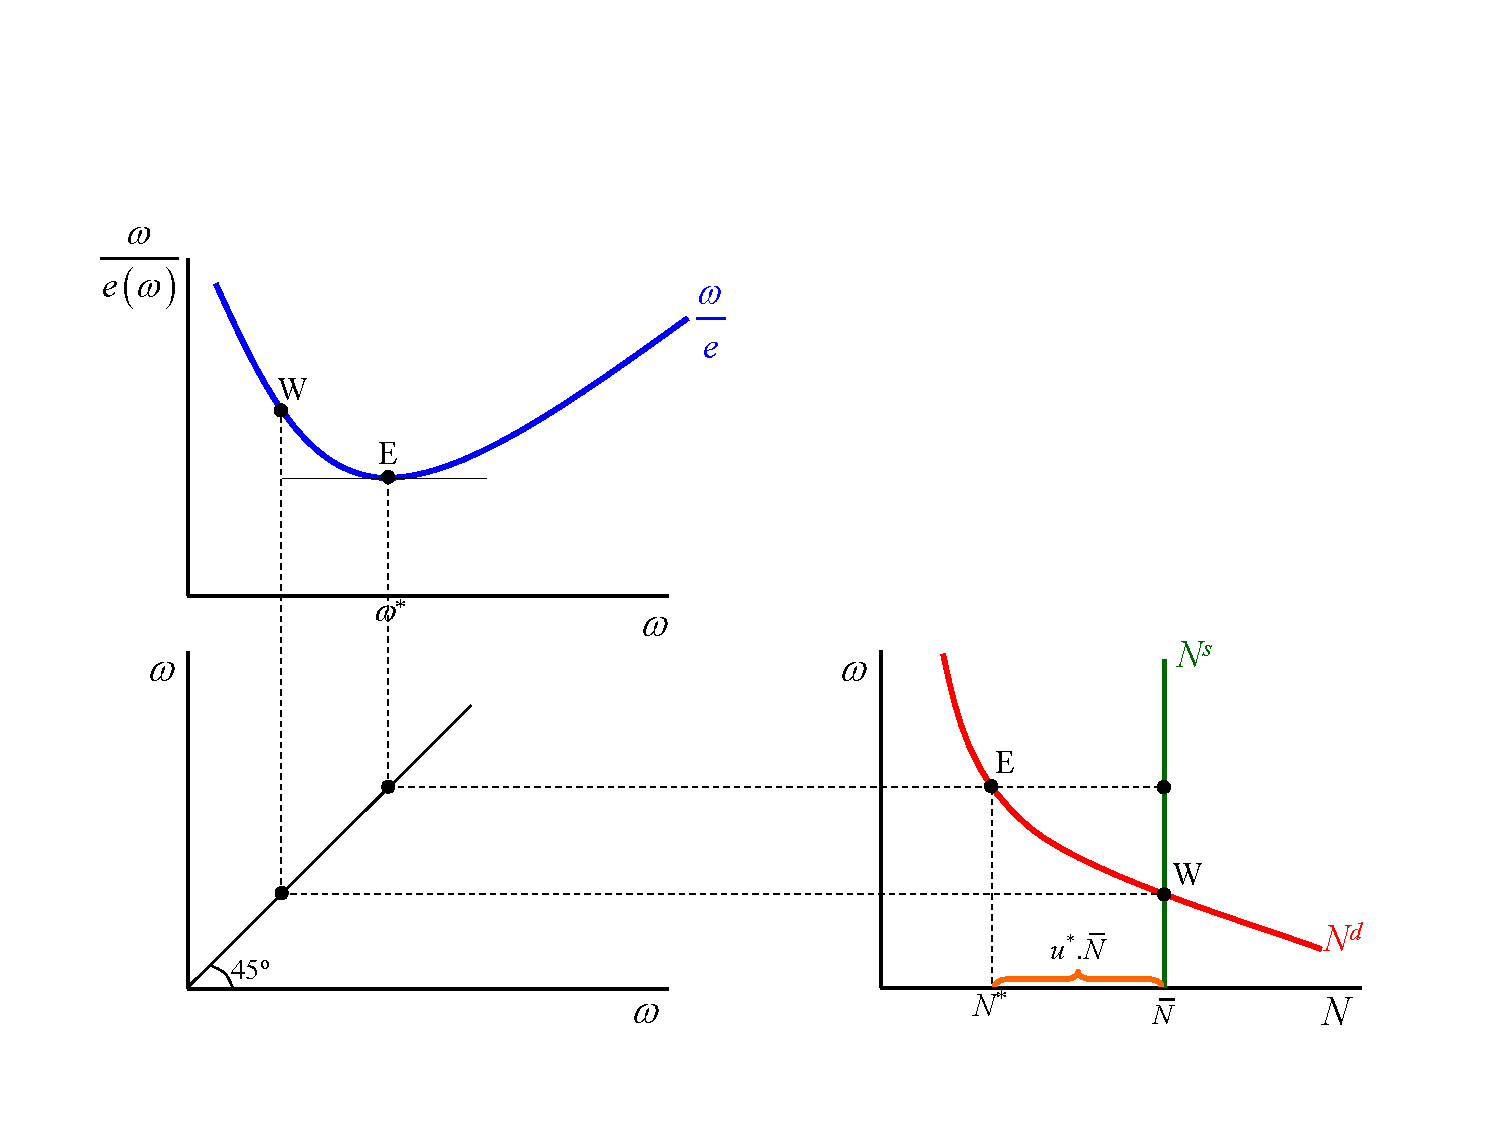
\includegraphics[max width=\linewidth]{4_0_New_Keynesian_School/efficiency_wages_graph.pdf}
    \caption{Efficiency wages and involuntary unemployment}  
\end{figure}
\paragraph{A static model of effort supply faced by the firm}

Utility: $U=C^{\alpha}(1-e)^{1-\alpha}$ \\

Consumption: $C=B(1-S)+S\omega$

Where 
\[
S=\left\{
\begin{array}{ll}
      1 & \text{If employed} \\
      0 & \text{If unemployed}\\

\end{array} 
\right. \]

And B is the employment benefit, defined as $B< max(\omega ,\omega    (1-e)^{\frac{1-\alpha}{\alpha}})$. 
The following table summarizes the consumption, leisure, and utility for each individual, depending on their employment status.

\begin{table}[H]
\begin{tabu} to \linewidth{|X[-2.5,c,m]|X[c,m]|X[c,m]|X[c,m]|}
\tabucline-
   Individual & Consumption (C) & Leisure (Z) & Utility(U)  \\ \hline
    Non-Shirker (N) & $\omega$ & $1-\overline{e}$ & $U_{S}=\omega^{\alpha}(1-\overline{e})^{1-\alpha}$ \\ \hline
    Shirker (S) & $\omega$ & 1-0 & $U_{N}=\omega^{\alpha}$  \\ \hline
    Unemployed(U) & B & 1-0 & $U_{U}=B^{\alpha}$\\
    \hline
\end{tabu}
\caption{Outcomes for participants}
\end{table}

Note $U_{U}<U_{N}<U_{S}$.

\begin{itemize}
    \item $0 \leq u \leq 1$ is the unemployment rate, i.e. the probability of not finding a new job. 
    \item $0\leq q \leq 1$ is the probability of being caught shirking 
\end{itemize}


\begin{figure}[ht]

\centering
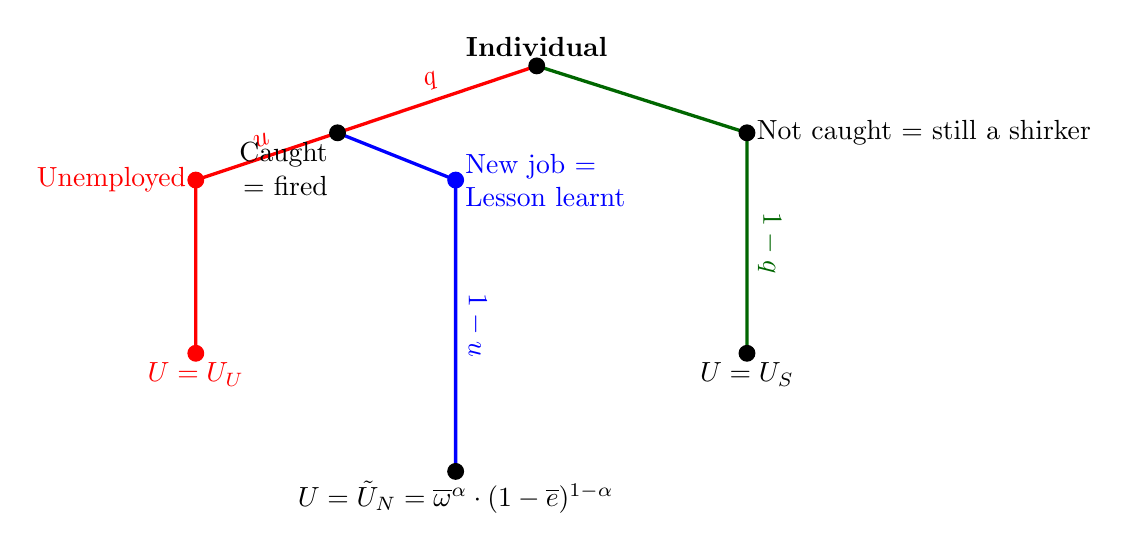
\begin{tikzpicture}[scale=1]


\coordinate (a) at (3.83, 2.65);
\coordinate (c) at (1.3, 1.8);
\coordinate (d) at (2.8, -2.5);
\coordinate (e) at (-0.5,-1);
\coordinate (f) at (6.5, -1);
\coordinate (g) at (-0.5, 1.2);
\coordinate (h) at (2.8, 1.2);



\draw [very thick, red] (e) -- (g) -- (c) node[pos=0.5,sloped,above] {$u$};
\draw [very thick, red] (a) -- (c) node[pos=0.5,sloped,above] {$q$}; 




\draw [very thick, black!60!green] (a) -- (6.5, 1.8) -- (f) node[pos=0.5,sloped,above] {$1-q$};



\draw [very thick, blue] (c) -- (h) -- (d) node[pos=0.5,sloped,above] {$1-u$};


\draw [fill] (c) circle [radius=0.1] node [below left, align = right] {Caught \\ = fired};
\draw [fill] (6.5, 1.8) circle [radius=0.1] node  [right] {Not caught = still a shirker};
\draw [fill = black] (a) circle [radius=0.1] node [above] {\textbf{Individual}};
\draw [fill] (d) circle [radius=0.1] node [below] {$U = \tilde { U } _ { N } = \overline { \omega } ^ { \alpha } \cdot ( 1 - \overline { e } ) ^ { 1 - \alpha }$};
\draw [fill, red] (e) circle [radius=0.1] node [below] { $U = U_U$};
\draw [fill] (f) circle [radius=0.1] node [below] {$U = U_S$};
\draw [fill, red] (g) circle [radius=0.1] node [left] {Unemployed};
\draw [fill, blue, align = left] (h) circle [radius=0.1] node [right] {New job = \\ Lesson learnt};

\end{tikzpicture}
\caption{Decision tree for a shirker}
\end{figure}



\begin{equation*}
\begin{aligned}
    E(U_{S})=q[(1-u).\Tilde{U}_{N}+u.U_{U}]+(1+q)U_{S} \\
  &&& \texttt{Where} &&& \overline{V}=(1-u).\Tilde{U}_{N}+uU_{U} \\
\end{aligned}
\end{equation*}

\begin{equation*}
\begin{aligned}
    \overline{V}=(1-u)[\overline{\omega}^{\alpha}(1-\overline{e})^{1-\alpha}]+uB^{\alpha} \\
    q.\overline{V}+(1-q)\omega^{\alpha}=\omega^{\alpha}.\overline{V}(1-\overline{e})^{1-\alpha}
\end{aligned}
\end{equation*}

Note that $E(U_{S}\leq U_{N}$. Replacing $\overline{V}$ in $E(U_{S})$: 

\begin{equation*}
    q.\overline{V}+(1-q)\omega^{\alpha}=\omega^{\alpha}.\overline{V}(1-\overline{e}^{1-\alpha}
\end{equation*}

Solving for $\omega$ we get the No-Shirking Condition for an individual firm: 

\begin{equation}\label{NSC_firm}
    \omega=\bigg[ \frac{q.\overline{V}}{(1-\overline{e})^{1-\alpha-(1-q)}} \bigg]
\end{equation}
By assumption, $q>1-(1-\overline{e})^{1-\alpha}$ \\
To see the NSC graphically: 

\begin{figure}[H]
\centering
\begin{tikzpicture}[scale=1.5]

% Axis

\draw [ultra thick](0,0) -- (8,0);

\draw [ultra thick](0,0) -- (0,5.5);

\node [left] at (-0.2,5.3) {$\omega$};
\node [below left] at (0,0) {$0$};

\node [below] at (8.2,-0.2) {$1 - u$};

\node [left] at (0,1) {$\left[ \frac { q B ^ { \alpha } } { ( 1 - \overline { e } ) ^ { 1 - \alpha } - ( 1 - q ) } \right] ^ { \frac { 1 } { \alpha } }$};


\node [left] at (0,3.5) {$\left[ \frac { q \cdot \overline { \omega } ^ { \alpha } \cdot ( 1 - \overline { e } ) ^ { 1 - \alpha } } { ( 1 - \overline { e } ) ^ { 1- \alpha } - ( 1 - q ) } \right] ^ { \frac { 1 } { \alpha } }$};

%Curve
\draw[very thick, blue] (0,1) to [out=5,in=220]  (6,3.5) node[right]{$NSC_i$};
\draw [dashed] (0,3.5) -- (6,3.5);
\draw [dashed] (6,5)--(6,0)node[below]{$1$};
\end{tikzpicture}

\caption{NSC for an individual firm}

\end{figure}


\begin{equation*}
    \Tilde{U}_{N}>U_{U} \implies \frac{\partial\overline{V}}{\partial(1-u)>0}\implies \frac{\partial\omega}{\partial(1-u)}>0
\end{equation*}

From here we can derive the macroeconomic No-Shirking Condition:

\begin{equation}\label{NSC_macro}
    \omega=\bigg[\frac{quB^{\alpha}}{(1-\overline{e})^{1-\alpha}[1-q(1-u)]-(1-q)} \bigg]
\end{equation}

\begin{figure}[H]
\centering
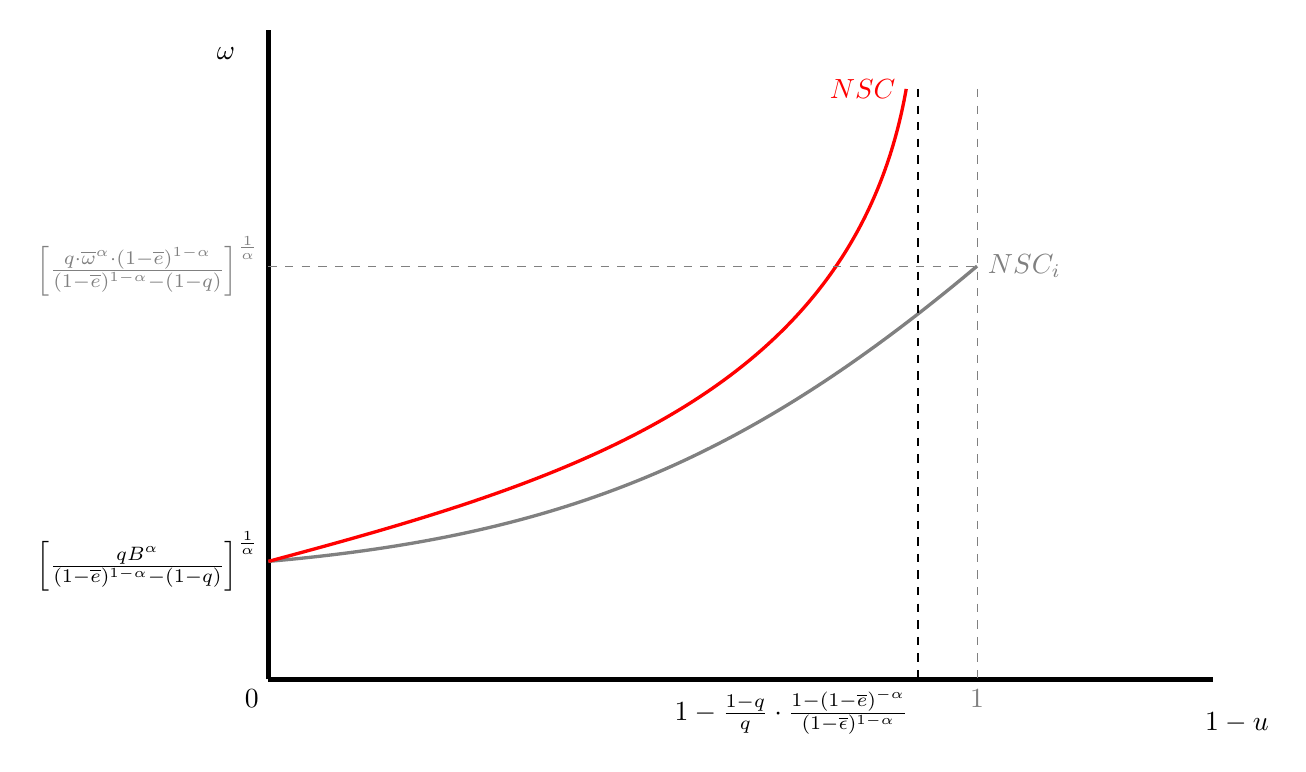
\begin{tikzpicture}[scale=1.5]

% Axis

\draw [ultra thick](0,0) -- (8,0);

\draw [ultra thick](0,0) -- (0,5.5);

\node [left] at (-0.2,5.3) {$\omega$};

\node [below] at (8.2,-0.2) {$1 - u$};
\node [below left] at (0,0) {$0$};

\node [left] at (0,1) {$\left[ \frac { q B ^ { \alpha } } { ( 1 - \overline { e } ) ^ { 1 - \alpha } - ( 1 - q ) } \right] ^ { \frac { 1 } { \alpha } }$};


\node[gray] [left] at (0,3.5) {$\left[ \frac { q \cdot \overline { \omega } ^ { \alpha } \cdot ( 1 - \overline { e } ) ^ { 1 - \alpha } } { ( 1 - \overline { e } ) ^ { 1- \alpha } - ( 1 - q ) } \right] ^ { \frac { 1 } { \alpha } }$};

%Curve
\draw[very thick, gray] (0,1) to [out=5,in=220]  (6,3.5) node[right]{$NSC_i$};
\draw[very thick, red] (0,1) to [out=15,in=260]  (5.4,5) node[left]{$NSC$};

\draw [dashed, gray] (0,3.5) -- (6,3.5);
\draw [dashed, gray] (6,5)--(6,0)node[below]{$1$};
\draw [dashed] (5.5,5)--(5.5,0)node[below left]{$1 - \frac { 1 - q } { q } \cdot \frac { 1 - ( 1 - \overline { e } ) ^ { - \alpha } } { ( 1 - \overline { \epsilon } ) ^ {1 - \alpha } }$};
\end{tikzpicture}

\caption{Macroeconomic NSC}

\end{figure}

This is just one side of the equilibrium, however, so we must calculate a labour demand in order to achieve an actual equilibrium. 
\begin{equation}\label{Inv_Labour_Demand}
    Af'(L)=\frac{\omega}{\overline{e}} \implies \omega=\overline{e}Af'\big[\overline{e}(1-u)\overline{N}\big]
\end{equation}
This is the inverse labour demand for employees. Note that it is decreasing because the marginal productivity of labour is decreasing as well. 


\begin{equation*}
 \left. \omega \right\rvert_{NSC} = \bigg[\frac{q.u}{Z(u,q)}\bigg]^{\frac{1}{\alpha}}B 
\end{equation*}

We can see the relation of the real wage to the unemployment rate, the employment benefits, and the probability of being caught shirking, as the derivatives of the last equation, 

\begin{equation*}
    \begin{aligned}
        \frac{\partial\left. \omega \right\rvert_{NSC}}{\partial u}<0 \\
        \frac{\partial\left. \omega \right\rvert_{NSC}}{\partial B}>0 \\
        \frac{\partial\left. \omega \right\rvert_{NSC}}{\partial q}<0
    \end{aligned}
\end{equation*}

To wrap up, comes the graphic for the equilibrium, and the effect of shocks: 
\begin{figure}[H]
\centering
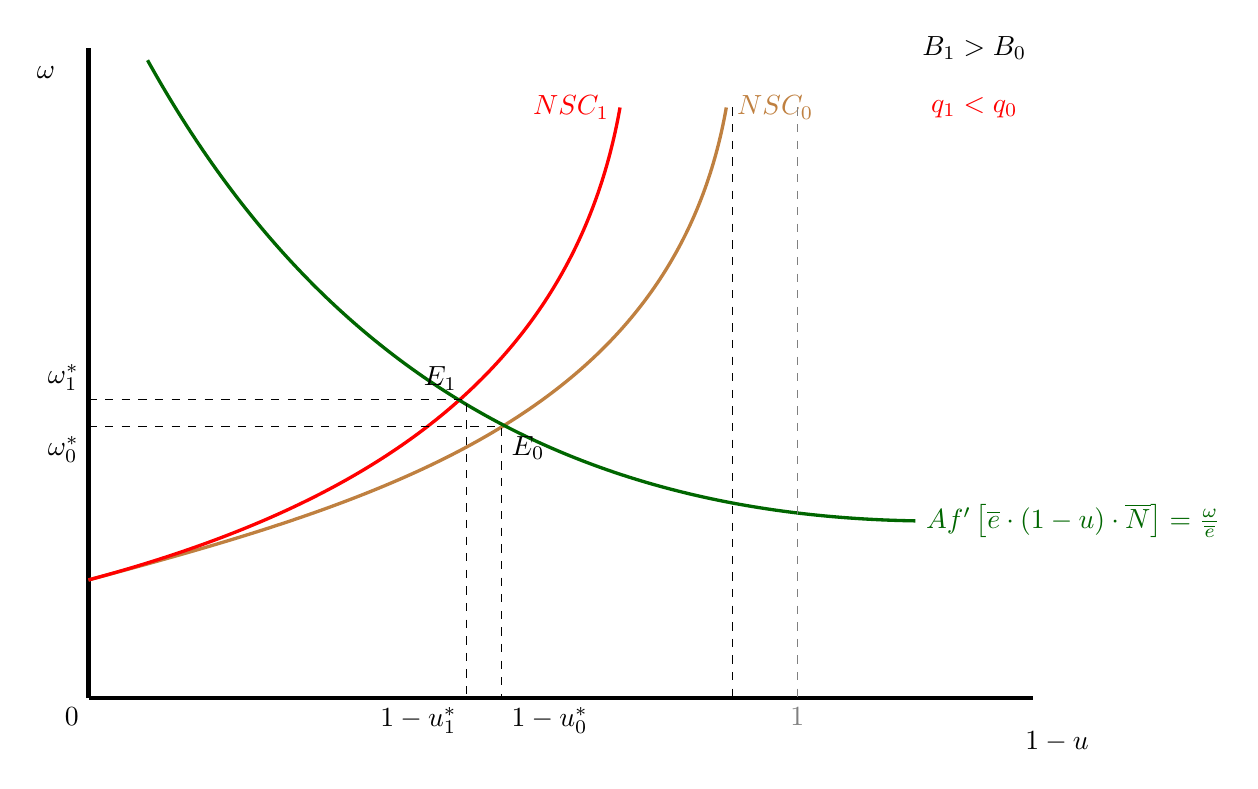
\begin{tikzpicture}[scale=1.5]

% Axis

\draw [ultra thick](0,0) -- (8,0);

\draw [ultra thick](0,0) -- (0,5.5);

\node [left] at (-0.2,5.3) {$\omega$};

\node [below] at (8.2,-0.2) {$1 - u$};
\node [below left] at (0,0) {$0$};

%\node [left] at (0,1) {$\left[ \frac { q B ^ { \alpha } } { ( 1 - \overline { e } ) ^ { 1 - \alpha } - ( 1 - q ) } \right] ^ { \frac { 1 } { \alpha } }$};


%\node[gray] [left] at (0,3.5) {$\left[ \frac { q \cdot \overline { \omega } ^ { \alpha } \cdot ( 1 - \overline { e } ) ^ { 1 - \alpha } } { ( 1 - \overline { e } ) ^ { 1- \alpha } - ( 1 - q ) } \right] ^ { \frac { 1 } { \alpha } }$};

%Curve
\draw[very thick, brown] (0,1) to [out=15,in=260]  (5.4,5) node[right]{$NSC_0$};
\draw[very thick, red] (0,1) to [out=15,in=260]  (4.5,5) node[left]{$NSC_1$};
\draw[very thick, black!60!green] (0.5, 5.4) to [bend right = 30] (7,1.5) node [ right] {$Af ^ { \prime } \left[ \overline { e } \cdot ( 1 - u ) \cdot \overline { N } \right] = \frac { \omega } { \overline { e } }$};

\draw [dashed] (5.45,5)--(5.45,0);

\draw [dashed] (0,2.525) node[above left]{$\omega^*_1$}  -- (3.2,2.525) node[above left]{$E_1$} -- (3.2, 0) node[below left] {$1 - u^*_1$};

\draw [dashed] (0,2.3) node[below left]{$\omega^*_0$} -- (3.5,2.3) node[below right] {$E_0$} -- (3.5, 0) node[below right] {$1 - u^*_0$}  ;


\node at (7.5,5.5) {$B_1 > B_0$};
\node [red] at (7.5,5) {$q_1 < q_0$};


\draw [dashed, gray] (6,5)--(6,0)node[below]{$1$};
\end{tikzpicture}

\caption{Equilibrium and shocks to the NSC}

\end{figure}


A negative shock to q, as in the graph, $q_{1}<q_{0}$ moves the NSC to the left, resulting in a higher real wage for workers, but reducing overall employment. A positive shock to unemployment benefits, as $B_{1}>B_{0}$, moves the right, making the real wage lower, but resulting in more employment.  

\newpage
\subsection{Search and Matching Model}
\subsubsection{The matching function}
\begin{equation}\label{Matching_function}
    M_{t}=M(u_{t}.L_{t},V_{t}.L_{t})
\end{equation}

Define $x=u.L, V.L$

\begin{itemize}
    \item $\frac{\partial M}{\partial x}>0$
    \item $\frac{\partial^{2}M}{\partial x^{2}}<0$
    \item $\frac{\partial^{2}}{\partial(u.L)}\frac{\partial^{2}}{\partial(V.L}-\frac{\partial^{2}M}{\partial(u.L\partial(V.L)}>0$
\end{itemize}

\begin{itemize}
    \item $M(\lambda u.L, \lambda v.L>\lambda M(u.L,V.L) \implies$ Thick market condition
    \item $M(\lambda u.L, \lambda v.L<\lambda M(u.L,V.L) \implies$ Crowding effects
\end{itemize}

\begin{equation*}
\begin{aligned}
    M_{t}=\xi(u_{t}.L_{t})^{1-\eta}(V_{t}L_{t})^{\eta} \\
    M_{t}=\xi u_{t}^{1-\eta}V_{t}^{\eta}L_{t} 
\end{aligned}
\end{equation*}

\begin{equation*}
\begin{aligned}
    m_{t}=\frac{M_{t}}{L_{t}}=\xi u_{t}^{1-\eta}V_{t}^{\eta} \implies v_{t}=\big(\frac{m_{t}}{\xi}\big)^{\frac{1}{\eta}}u_{t}^{-\frac{1-\eta}{\eta}}
\end{aligned}
\end{equation*}
$v_{t}=\big(\frac{m_{t}}{\xi}\big)^{\frac{1}{\eta}}u_{t}^{-\frac{1-\eta}{\eta}}$ is known as the Beveridge curve, and $\frac{m_{t}}{\xi}$ is a measure for the level of frictions in the labour market. 

\subsubsection{Labour-Market flows: Mortensen-Pisserides}
\begin{equation*}
\begin{aligned}
    \Delta N_{t+1}^{*}=M_{t} -\lambda N_{t}^{*} \\
    m_{t}=\xi\big(\frac{V_{t}}{u_{t}}\big)^{\eta}u_{t} \\
    m_{t}=\xi\theta_{t}^{\eta}u_{t}
\end{aligned}  
\end{equation*}

Where $\theta_{t}=\frac{v_{t}L_{t}}{u_{t}l_{t}}=\frac{v_{t}}{u_{t}}$ is the tightness ration.

We can define the job finding rate:
\begin{equation}\label{JFR}
    \phi_{t}=\frac{M_{t}}{u_{t}L_{t}}=\frac{m_{t}}{u_{t}}=\xi \theta_{t}^{\eta}
\end{equation}

And the vacancy filling rate: 
\begin{equation}\label{VFR}
    \beta_{t}=\frac{M_{t}}{u_{t}L_{t}}=...=\xi\theta_{t}^{\eta-1}
\end{equation}

\begin{equation*}
    \frac{\Delta N_{t+1}^{*}}{L_{t}}=m_{t}-\lambda(1-u_{t})=\xi\theta_{t}^{\eta}u_{t}-\lambda(1-u_{t})
\end{equation*}

\subsubsection{Intertemporal Optimization}

\begin{equation*}
    \mathcal{V}_{t}=E_{t}\sum_{\tau=t}^{\infty}(1+\rho)^{-(\tau-t)}.V_{\tau} 
\end{equation*}

\begin{equation*}
    \mathcal{V}_{t}=V_{t}+E_{t}\sum_{\tau=t+1}^{\infty}(1+\rho)^{-(\tau-t)}.V_{\tau} 
\end{equation*}

\begin{equation*}
    \mathcal{V}_{t}=V_{t}+\frac{1}{1+\rho}\sum_{\tau=t+1}^{\infty}(1+\rho)^{-[\tau-(t+1)]}.V_{t} 
\end{equation*}

\begin{equation*}
    \mathcal{V}_{t}=V_{t}+\frac{1}{1+\rho}\mathcal{V}_{t+1}
\end{equation*}

\subsubsection{Firms}
\begin{equation*}
y_{t}=A_{t}.N_{t}-\Phi
\end{equation*}
Firms produce only with labour, and we normalize their number of workers to one, so $N_{t}$ can only be one of two values: 

\[ 
N_{t}=\left\{
\begin{array}{l l}
    1 & \text{position filled (F)}  \\
    0 & \text {position vacant (V)}
\end{array}
\right.
\]
And so profits can also take one of only two values: 
\[ 
\pi_{t}=\left\{
\begin{array}{cc}
    \pi_{t}^{F}=A_{t}-\Phi-\omega_{t} & N_{t}=1  \\
     \pi_{t}^{V}=-\Phi & N_{t}=0 
\end{array}
\right.
\]

\begin{enumerate}
    \item $\mathcal{V}_{t}^{F}=\pi_{t}^{F}+\frac{1}{1+\rho}\bigg[(1-\lambda)\mathcal{V}_{t+1}^{F}+\lambda\mathcal{V}_{t+1}^{V} \bigg]$
    \item $\mathcal{V}_{t}^{V}=\pi^{V}_{t}=\frac{1}{1+\rho}\bigg[(1+\beta_{t+1})\mathcal{V}_{t+1}^{V}+\beta_{t+1}\mathcal{V}_{t+1}^{F} \bigg]$
\end{enumerate}

\subsubsection{Households}
\[ 
U_{t}=\left\{
\begin{array}{l l}
     U_{t}^{E}=\omega_{t} & L_{t}=1  \\
     U_{t}^{U}=B & L_{t}=0 
\end{array}
\right.
\]

$B< min [\omega_{t}, A_{t}]$

\begin{enumerate}
    \item $\mathcal{V}_{t}^{E}=\omega_{t}+\frac{1}{1+\rho}\bigg[ (1-\lambda)\mathcal{V}_{t+1}^{E}+\lambda\mathcal{V}_{t+1}^{U} \bigg] $, where, $\omega_{t}=U_{t}^{E}$
    \item $\mathcal{V}_{t}^{U}=B+\frac{1}{1+\rho}\bigg[ (1-\phi_{t+1})\mathcal{V}_{t+1}^{U}+\phi_{t+1}\mathcal{V}_{t+1}^{E} \bigg] $
\end{enumerate}

\subsubsection{Bargaining}
\begin{equation*}
\begin{aligned}
    \underset{{\mathcal{P}^{V}},\mathcal{P}^{U}}{max} & (\mathcal{V}_{t}^{F}-\mathcal{V}_{t}^{V})^{\varepsilon}(\mathcal{V}_{t}^{E}-\mathcal{V}_{t}^{U})^{1-\varepsilon} \\
    s.t. & \mathcal{P}^{V}+\mathcal{P}^{U}=\mathcal{P}_{t}
\end{aligned}
\end{equation*}
Note that $\mathcal{V}_{t}^{F}-\mathcal{V}_{t}^{V}=\mathcal{P}^{V}$, and, $\mathcal{V}_{t}^{E}-\mathcal{V}_{t}^{U}=\mathcal{P}^{U}$.
\paragraph{} 
From the first order conditions we get the Nash bargaining solution: 

\begin{equation}\label{Nas_Barg_Solution}
    \frac{\mathcal{P}_{t}^{U}}{\mathcal{P}_{t}^{V}}=\frac{1-\varepsilon}{\varepsilon}
\end{equation}

\subsubsection{Steady State}
We evaluate the system dynamics only at a steady state. For this purpose we'll compute the variables at a steady state. 

\begin{equation*}
    \Delta N_{t+1}^{*}=0 \implies o=\xi . \theta^{\eta}.u-\lambda(1-u) \implies u=\frac{\lambda}{\lambda + \xi.\theta^{\eta}}
\end{equation*}

Note: $\xi.\theta^{\eta}=\phi$ which is the Job finding rate. 

\begin{equation*}
\begin{aligned}
    \mathcal{V}^{V}=-\frac{1+\rho}{\rho+\beta}.\Phi+\frac{\beta}{\rho+\beta}.\mathcal{V}^{F} \\
    + \\
    \mathcal{V}^{F}=\frac{(1+\rho)(\rho+\beta)}{\rho(\rho+\beta+\lambda)}(A-\omega)-\frac{1+\rho}{\rho}\Phi \\ 
    = \\
    \mathcal{V}^{V}=-\frac{1+\rho}{\rho}.\Phi+\frac{\beta(1+\rho)}{\rho(\rho+\beta+\lambda)}(A-\omega) \\
   \implies \mathcal{P}^{V}=\mathcal{V}^{F}-\mathcal{V}^{V}=...=\frac{1-\rho}{\rho+\lambda+\beta}(A-\omega)
\end{aligned}
\end{equation*}

\begin{equation*}
\begin{aligned}
    \mathcal{V}^{E}=\frac{1+\rho}{\rho+\lambda}\omega+\frac{\lambda}{\rho+\lambda}\mathcal{V}^{U} \\ 
    + \\
    \mathcal{V}^{U}=\frac{(1+\rho)(\rho+\lambda)}{\rho+(\rho+\lambda+\phi<)} \\
    = \\
    \mathcal{V}^{E}=\frac{(1+\rho)(\rho+\phi)}{\rho(\rho+\lambda+\phi)}\omega+ \frac{\lambda(1+\rho)}{\rho(\rho+\lambda+\phi)}B \\
    \implies \mathcal{P}^{U}=\mathcal{V}^{E}-\mathcal{V}^{U}=...=\frac{1+\rho}{\rho+\lambda+\phi}(\omega-B)
\end{aligned}
\end{equation*}
We can now introduce these expressions in the Nash Bargaining Solution \ref{Nas_Barg_Solution};

\begin{equation*}
\begin{aligned}
    \frac{\mathcal{P}^{U}}{\mathcal{P}^{V}}=\frac{1-\varepsilon}{\varepsilon} \\
    \implies \omega=B+\frac{(1-\varepsilon)(\rho+\lambda+\phi)}{\rho+\lambda+(1-\varepsilon)\phi+\varepsilon\beta}
\end{aligned}
\end{equation*}

For $\phi=\beta \implies \omega-B=(1-\varepsilon)(A-B)$. Also, $\frac{\partial(\omega-B)}{\partial\beta}<0$.

\begin{equation*}
    \mathcal{V}^{V}=...=-\frac{1+\rho}{\rho}\Phi+\frac{\beta(1+\rho)\varepsilon}{\rho \big[\rho+\lambda+\phi(1-\varepsilon)+\varepsilon\beta \big]}(A-B)
\end{equation*}

\begin{equation*}
    u=\frac{\lambda}{\lambda +\xi\theta^{\eta}} \implies \theta=\bigg[\frac{\lambda(1-u)}{\xi u} \bigg]^{\frac{1}{\eta}}
\end{equation*}

Recall that $\beta$ in \ref{JFR} is the job finding rate (JFR), and $\phi$ in \ref{VFR} is the vacancy filling rate (VFR). 
\begin{equation*}
    \beta=\xi \bigg[\frac{\lambda(1-u)}{\xi u} \bigg]^{\frac{\eta-1}{\eta}} \implies \frac{\partial\beta}{\partial u}>0
\end{equation*}

\begin{equation*}
    \theta=\xi\frac{\lambda(1-u)}{\xi u} \implies \frac{\partial \phi}{\partial u}<0
\end{equation*}

\begin{equation*}
    \begin{aligned}
        \mathcal{V}^{V}=-\frac{\rho+1}{\rho}.\Phi+\frac{1+\rho}{\rho}\frac{\varepsilon\beta(u)}{\rho+\lambda+(1-\varepsilon)\phi(u)+\varepsilon\beta(u)}
    \end{aligned}
\end{equation*}
\begin{equation*}
     \mathcal{V}^{V}=-\frac{1+\rho}{\rho}\Phi+h(u)
\end{equation*}
$h'(u)>0$

\subsubsection{Free entry}
\begin{equation*}
    \mathcal{V}^{V}=0
\end{equation*}
\begin{equation*}
    0=-\frac{1+\rho}{\rho}.\Phi+h(u) \implies u^{*}=h^{-1}\big(\frac{1+\rho}{\rho}\Phi
\end{equation*}

\subsubsection{Changes in Productivity and Unemployment benefits}
\begin{equation*}
    \frac{\partial h}{\partial(A-B)}>0
\end{equation*}

\subsubsection{Welfare}
$L_{t}=L_{0}$

\begin{equation*}
    \frac{\Delta N_{t+1}}{L_{t}}=\frac{N_{t+1}^{*}-N_{t}^{*}}{L_{0}}=\frac{(1-u_{t-1})L_{0}-(1-u_{t})L_{0}}{L_{0}}=-\Delta u_{t+1}
\end{equation*}

\begin{equation*}
    \begin{aligned}
        \underset{u_{t},V_{t}}{max}\sum_{\tau=t}^{\infty}(1+\rho)^{-(\tau-t)}\bigg[(A_{t}-\Phi)(1-u_{t})+Bu_{t}-\Phi V_{t} \bigg] \\
    &   s.t. \Delta u_{t+1}=\lambda (1-u_{t}) - \xi V_{t}^{\eta}u_{t}^{1-\eta}
    \end{aligned}
\end{equation*}

\begin{equation*}
    H=(A_{t}-\Phi)(1-u_{t})+Bu_{t}-\Phi V_{t}+\mu_{t}\big[\lambda(1-u_{t})-\xi u_{t}^{1-\eta}V_{t}^{\eta} \big]
\end{equation*}

\begin{enumerate}
    \item $\frac{\partial H}{\partial V}= 0 \implies -\Phi-\mu_{t}\eta\xi u_{t}^{1-\eta} V_{t}^{\eta-1}=0$
    \item $\frac{\partial H}{\partial u}=0 \implies -(A_{t}-\Phi)+B-\mu_{t}\lambda u_{t}(1-\eta)\xi\mu_{t}^{-\eta}V_{t}^{\eta}=0$
\end{enumerate}

\begin{enumerate}
    \item $\mu.\eta.\xi.\big(\frac{V}{u}\big)^{\eta-1}=-\Phi \implies \mu=\frac{-\Phi}{\eta\beta}$. Note that $\frac{V}{u}=\theta$, and $\xi\big(\frac{V}{u}\big)^{\eta-1}=\beta(\theta)$ 
    \item $-(A-\Phi-B)=\big[\rho+\lambda+(1-\eta).\xi.(\frac{V}{u})^{\eta} \big].\mu \implies A-B=\frac{\lambda+\rho+(1+\eta).\phi+\eta.\beta}{\eta.\beta}.\Phi$. This gives us the Welfare-Maximizing solution for the central planner.
\end{enumerate}

\begin{equation*}
    \begin{aligned}
        \mathcal{V}^{V}=0 \\ \implies-\frac{1+\rho}{\rho}.\Phi+\frac{1+\rho}{\rho}.(a-B).\frac{\varepsilon\beta}{\lambda+\rho+(1-\varepsilon)\phi+\varepsilon\beta}=0 \\
        \implies A-B=\frac{\lambda+\rho+(1-\varepsilon)\Phi+\varepsilon\beta}{\varepsilon.\beta}.\Phi 
    \end{aligned}
\end{equation*}
Which is the decentralized equilibrium. 
\paragraph{} 
We can see the two are different, except for the case of $\eta=\varepsilon$ (Hosios solution), which is a very specific and sensitive situation, where a small deviation in one of the variables will put the economy in a different equilibrium. 






\newpage
\chapter{The New Macroeconomics}

\section{Problems and Puzzles}

Central questions of the validity of previous models etc. 
\begin{center}
    

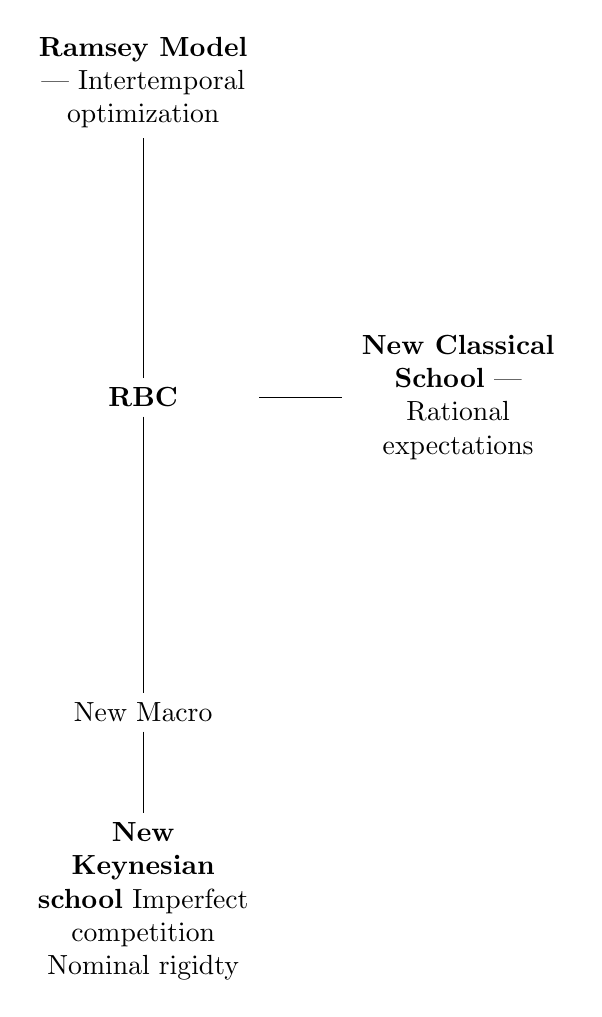
\begin{tikzpicture}[scale=0.8, grow cyclic, text width=2.7cm, align=flush center,
	level 1/.style={level distance=5cm,sibling angle=90},
	level 2/.style={level distance=3cm,sibling angle=45}]
 \node{\textbf{RBC}}
 	  	child { node {New Macro}
	        child { node {\textbf{New Keynesian school}
	        Imperfect competition
	        Nominal rigidty}}
	        }
	child { node {\textbf{New Classical School} --- Rational expectations}}
	child { node {\textbf{Ramsey Model} --- Intertemporal optimization }
	               }

;
\end{tikzpicture}
 \end{center}

\newpage
\section{The new keynesian-neoclassical synthesis}
\subsection{The Dixit-Stiglitz-Ramsay Model}
\subsubsection{The Model's structure} 

\paragraph{Households}

\begin{equation*}
\begin{aligned}
    \underset{C,L,c_{j}}{max}U=\int_{0}^{\infty}e^{-\rho t}\bigg[\frac{C^{1-\theta}-1}{1-\theta}+V(1-L) \bigg].dL \\
    s.t. \Dot{K}=w.L+R.K+\pi-C-T-\delta.K \\
    C=n^{\frac{1}{1-\sigma}}\bigg[\int_{0}^{n}c(j)^{\frac{\sigma-1}{\sigma}}.dj \bigg]^{\frac{\sigma}{\sigma-1}}
\end{aligned}
\end{equation*}

With, $V'(.)>0$ and $V''(.)<0$.
\paragraph{}
To solve the optimization problem, we get a Current Value Hamiltonian (CVH): 
\begin{equation*}
    H=u+\lambda\Dot{K}
\end{equation*}
And the F.O.C's come as:
\begin{enumerate}
    \item $\frac{\partial H}{\partial C}=0 \implies C^{-\theta}-\lambda=0$
    \item $\frac{\partial H}{\partial L}=0 \implies -V'(1-L)+\lambda.w=0$
\end{enumerate}
And the transversality condition:
\begin{equation*}
    \lim_{t\to \infty}\Bigg[e^{-\rho.t}.\lambda(t).K(t) \bigg]=0
\end{equation*}
Rearranging the F.O.C's:
\begin{enumerate}
    \item Consumption Euler equation $\frac{\Dot{C}}{C}=\frac{1}{\theta}(r-\rho)$
    \item Frisch Labour Supply $V'(1-L)=C^{-\theta}.w$
\end{enumerate}

The consumption for a specific good j comes as $c(j)=\big(\frac{p(j)}{P}\big)^{-\sigma}.\frac{C}{N}$
\paragraph{}

\paragraph{Firms}

The production function for an individual firm comes as $g(j)-\Phi=F(K(j);L(j))$ and it's a regular neoclassical production function. However, the $\Phi$ is a fixed cost, which makes the function have positive returns to scale. 

\begin{equation*}
    \begin{aligned}
        (1-\mu)MPL=w && (1-\mu)MPK=R
    \end{aligned}
\end{equation*}

The aggregate production function, for the n firms in the market comes as $Y=F(K,L)-n\Phi$
\newline
\newline
\paragraph{Profits}

\begin{equation*}
        \pi=Y-w.L-R.K 
\end{equation*}
\begin{equation*}
    \pi=\big[F(K,L)-n\Phi \big]-(1-\mu)\big[\frac{\partial F}{\partial L}.L+\frac{\partial F}{\partial K}.K \big] \\
\end{equation*}
\begin{equation*}
        \pi=\mu.F(K,L)-n.\Phi 
\end{equation*}

  \paragraph{Capital Accumulation}
First consider the situation where firms aren't free to enter and leave the market: 

\begin{equation*}
    \begin{aligned}
        \Dot{K}=F(K,L)-n\Phi-C-G-\delta.K
    \end{aligned}
\end{equation*}
Note that $F(K,L)-n\Phi$ is equal to $w.L+R.K+\pi$
\newline

Now with free entry, companies will be entering the market until there are no more pure profits;

\begin{equation*}
    \begin{aligned}
        \pi=0 \implies n=\frac{\mu.F(K,L)}{\Phi}
    \end{aligned}
\end{equation*}

So capital accumulation comes as: 
\begin{equation*}
    \Dot{K}=(1-\mu).F(K,L)-C-G-\delta.K
\end{equation*}
Note that $(1-\mu).F(K,L)=Y$
\begin{figure}[H]
    \centering
    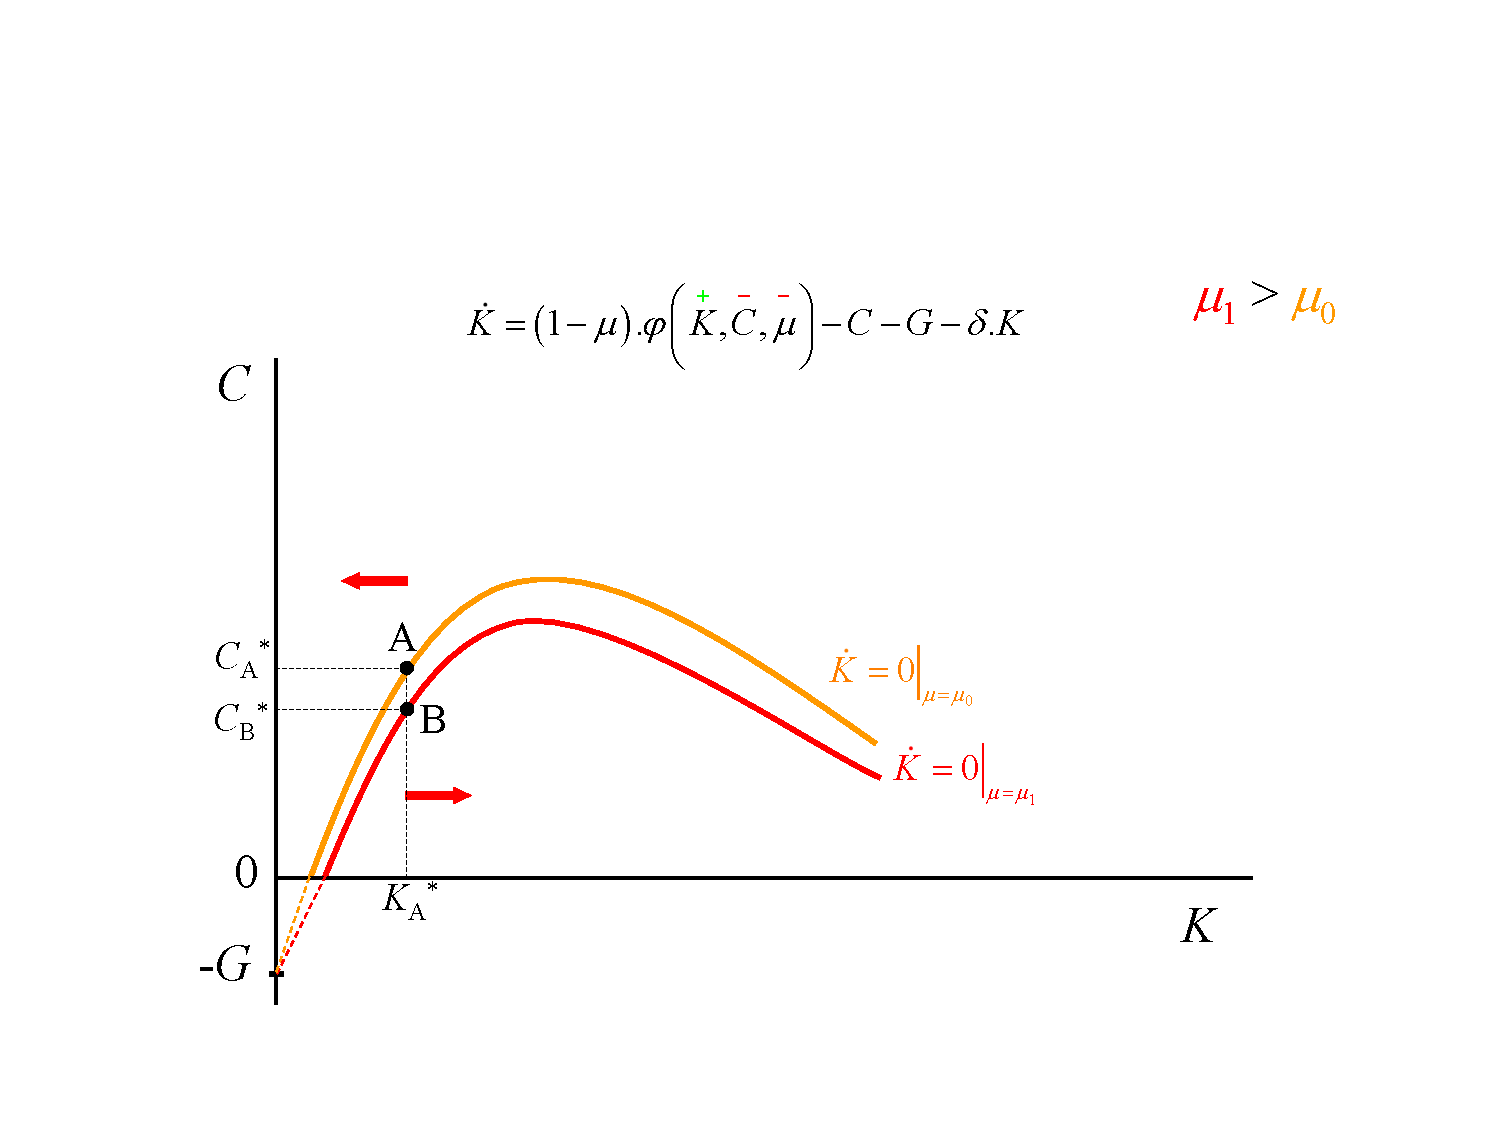
\includegraphics[max width=\linewidth]{5_0_The_New_Macroeconomics/Capital_accum_free_entry.pdf}
    \caption{Capital Accumulation with free entry}
    \label{Capital_Acc_free_entry}
\end{figure}

\paragraph{}
In order to get an equilibrium mapping capital and consumption, we'll reduce the equations of the model to take only these two variables into account, with the others still being relevant and having an impact, but getting a simpler model. 

\begin{equation*}
    r=R-\delta \implies r=(1-\mu).MPK-\delta
\end{equation*}
\begin{equation*}
    V'(1-L)=C^{-\theta}.w=C^{-\theta}(1-\mu).MPL(K,L)
\end{equation*}
\begin{equation*}
    L=\mathcal{L}(C,K,\mu)
\end{equation*}
$\mathcal{L}$ variates positively in $K$, and negatively in $C$ and $\mu$.
Replacing the L in $MPK(K,L)$ in $r$ by $\mathcal{L}$:
\begin{equation*}
        r=(1-\mu).MPK(K,\mathcal{L}(C,K,\mu))-\delta 
\end{equation*}
\begin{equation*}
        r=(1-\mu).\varphi_{K}(C,K,\mu)-\delta
\end{equation*}
Inserting these into the consumption Euler equation: 
\begin{equation*}
    \frac{\dot{C}}{C}=\frac{1}{\theta}\bigg[(1-\mu)\varphi_{K}(C,K,\mu)-\delta-\rho \bigg]
\end{equation*}
Note that $\varphi_{K}$ varies negatively on all parameters. 
\begin{figure}[H]
    \centering
    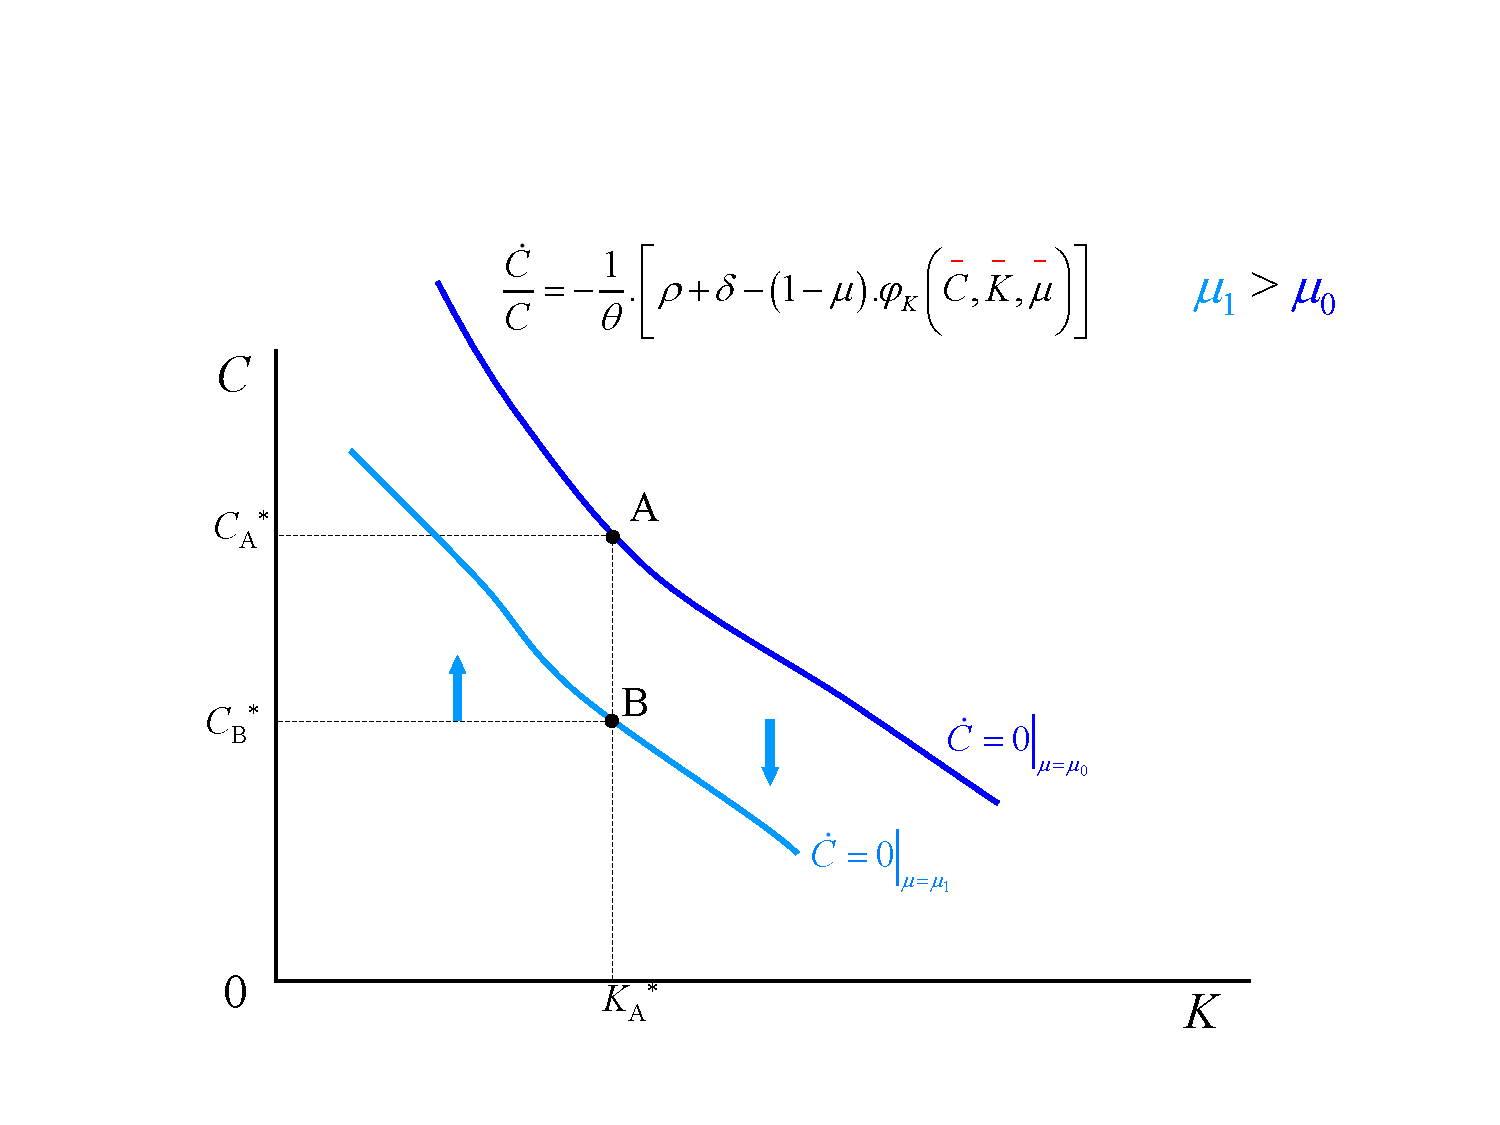
\includegraphics[max width=\linewidth]{5_0_The_New_Macroeconomics/Consumption_Euler_graph.pdf}
    \caption{Consumption Euler Equation and the Markup}
    \label{Consumption_Euler_Eq_Markup}
\end{figure}

 \paragraph{Steady State}
At a SS, $\dot{C}=0 \implies \varphi_{K}(C,K,\mu)=\frac{\rho+\delta}{1-\mu}$. 

\begin{equation*}
    F(K,L)=F(K,\mathcal{L}(C,K,\mu))=\varphi(K,C,\mu)
\end{equation*}
$\varphi(C,K,\mu)$ varies negatively in $\mu$ and $C$ because a higher $\mu$ or higher consumption result in less employment, and hence, less production. Varies positively in $K$ because more capital turns into more output. 

\begin{equation*}
\dot{C}=\dot{K}=0 \\
\implies C^{*}=\mathcal{C}(K^{*},\mu,G^{*})
\end{equation*}

$\mathcal{C}$ is positively impacted by $K^{*}$ and negatively by $\mu$ and $G^{*}$. 
In equilibrium:

\begin{equation*}
        (1-\mu)MPK(K^{*},L^{*})=\rho+\delta \\
\end{equation*}
\begin{equation*}
        (1-\mu)MPK \bigg[K^{*},\mathcal{L}(\mathcal{C}(K^{*},\mu,G^{*}),K^{*},\mu \bigg]=\rho+\delta
\end{equation*}
Define $\xi(K^{*}, \mu,G^{*})$, as $\xi(K^{*}, \mu,G^{*})= (1-\mu)MPK \bigg[K^{*},\mathcal{L}(\mathcal{C}(K^{*},\mu,G^{*}),K^{*},\mu \bigg]$. Capital and $\mu$ (the mark-up) have a negative impact in $\xi$, and government spending has a positive effect. 
\paragraph{}
See in the graph, a change in $\mu$ as $\mu_{1}>\mu_{0}$, moves $\xi$ down to the left, and makes the optimal level of capital lower.

\begin{figure}[H]
\centering
\begin{tikzpicture}[scale=1.5]

% Axis

\draw [thick](0,0) -- (8,0);

\draw [thick](0,0) -- (0,5.5);

\node [left] at (-0.2,5.3) {$\xi(K^{*},\mu,G^{*})$};

\node [below] at (8.2,-0.2) {$K$};

%Curve
\draw [thick] (1.1,5) to [out=285,in=155] (4.7,0.7) node[above]{$\xi_{1}$};
\draw [thick] (1.5,5) to [out=300,in=160] (6,1.5) node[above]{$\xi_{0}$};
\draw [thick] (0,2) -- (7,2) node[right]{$\rho+\delta$};
\draw [dashed] (2.8,2)--(2.8,0)node[below]{$K^{*}_{1}$};
\draw [dashed] (4.85,2)--(4.85,0)node[below]{$K^{*}_{0}$} ;
\end{tikzpicture}
\caption{Optimal Capital accumulation}

\end{figure}
\paragraph{Dynamics}

\begin{figure}[H]
    \centering
    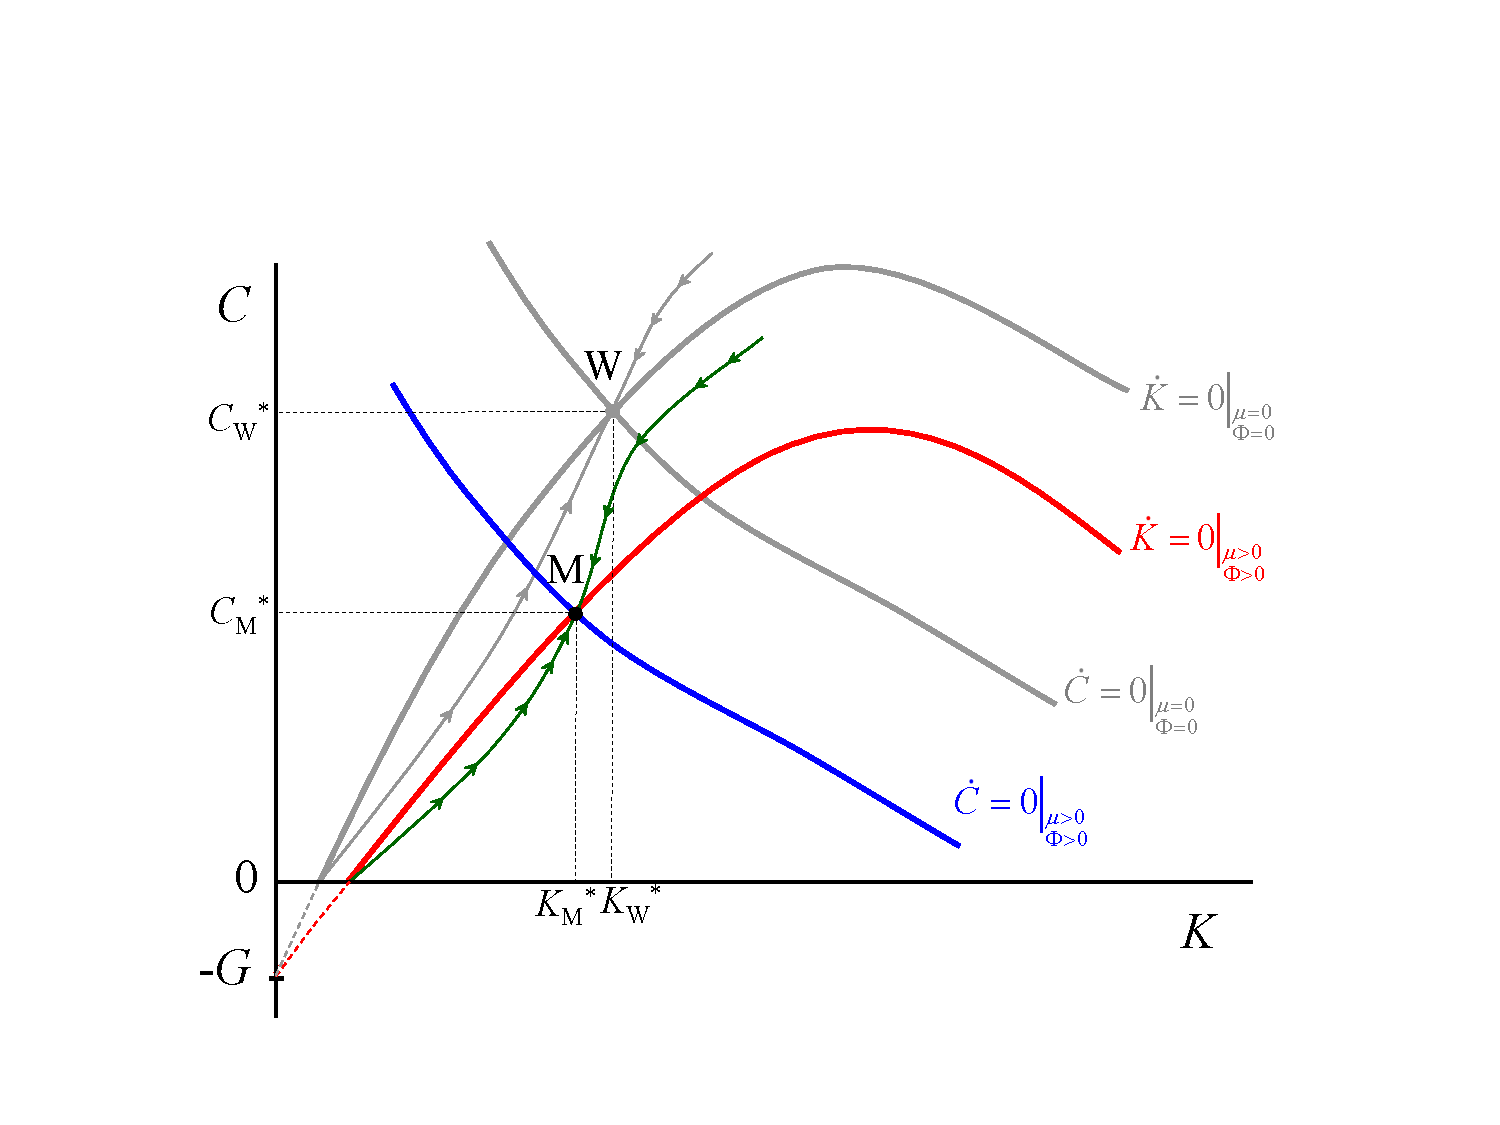
\includegraphics[max width=\linewidth]{5_0_The_New_Macroeconomics/long_run_eq.pdf}
    \caption{Long-run equilibrium in the Dixit-Stiglitz-Ramsey model with free entry}
    \label{LR_Equilibrium}
\end{figure}
Like in the Ramsay model, equilibrium isn't a single point, but an equilibrium path.

\paragraph{Fiscal Policy}

\begin{figure}[H]
    \centering
    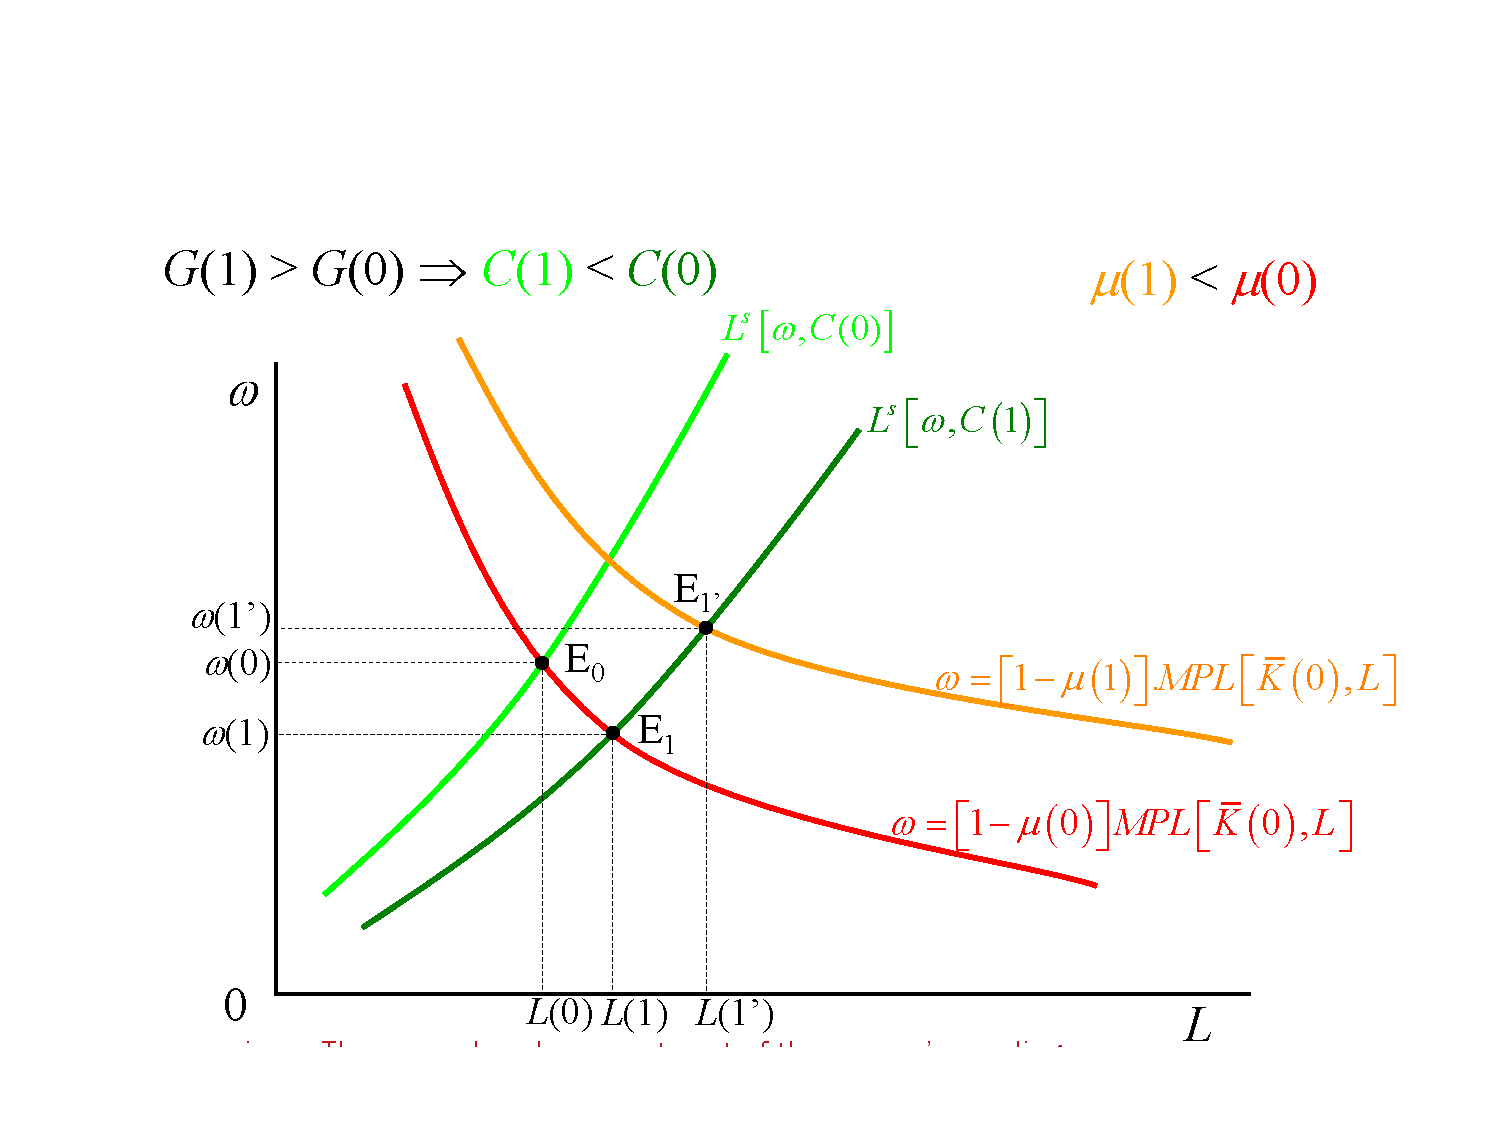
\includegraphics[max width=\linewidth]{5_0_The_New_Macroeconomics/Fiscal_Policy.pdf}
    \caption{Fiscal Policy, real wages, and the markup}
    \label{Fiscal_Policy}
\end{figure}

\paragraph{Measuring the Solow Residual} 
Introducing a measure of productivity $A$ in the production function: 
\begin{equation*}
    y(j)=A.\big[F(K(j),L(j))-\Phi \big]
\end{equation*}

And from that we get the aggregate production function: 
\begin{equation*}
    Y=A.F(K,L)-n.\Phi.A
\end{equation*}

\begin{equation*}
    \dot{Y}=\dot{A}.F+A\big[ \frac{\partial F}{\partial K}.\dot{K} + \frac{\partial F}{\partial L}.\dot{L} \big]-n.\Phi.\dot{A} 
\end{equation*}
\begin{equation*}
    \frac{\dot{Y}}{Y}=\frac{MPK.K}{Y}\frac{\dot{K}}{K}+\frac{MPL.L}{Y}.\frac{\dot{L}}{L}+\frac{(F-n\Phi).A}{Y}.\frac{\dot{A}}{A}
\end{equation*}

Note that $\frac{MPK.K}{Y}=\frac{Sh_{K}}{1-\mu}$ and $\frac{MPL.L}{Y}=\frac{Sh_{L}}{1-\mu}$.

\begin{equation*}
    g_{Y}=\frac{(1-\mu)MPK.K}{(1-\mu).Y}g_{K}+\frac{(1-\mu)MPL.L}{(1-\mu).Y}.g_{L}+g
\end{equation*}

Note that $(1-\mu)MPK=R$ and $(1-\mu)MPL=w$.

\begin{equation}\label{Output_growth}
    g_{Y}=\frac{1}{1-\mu}\big(Sh_{K}g_{K}+Sh_{L}.g_{L}\big)+g
\end{equation}

Because there can be pure profits, given the value of the markup, $Sh_{K}+Sh_{L}$ can be greater, smaller, or equal to 1, depending on the existence of pure profits. Recall $Y=w.L+R.K+\pi$; $Sh_{K}+Sh_{L}=1$ if there are no pure profits, $Sh_{K}+Sh_{L}\leq1$ if there are pure profits, and $Sh_{K}+Sh_{L}\geq 1$ if $\pi<0$.

\begin{equation*}
    \pi=y-(w.L+R.K)=\mu.A.F-n.\Phi.A
\end{equation*}
$w.L+R.K$ is the total cost (TC). This is because $\Phi$ is a total cost, but it's not necessarily a monetary cost, it's more of an inefficiency cost, resulting from the production function. This means that it's only a cost if the firm is actually producing. 

\begin{equation*}
    TC=(1-\mu).A.F
\end{equation*}
\begin{equation*}
    Sh_{L}=\frac{w.L}{Y}=\frac{w.L}{w.L+R.K}.\frac{w.L+R.K}{w.L+R.K+\pi}
\end{equation*}
The two fractions above have know values, depending on profits (for the second fraction) and on the production function you choose (for the first equation):
\[
\frac{w.L+R.K}{w.L+R.K+\pi}= \left\{
    \begin{array}{l}
         {\leq 1}  \longleftarrow \pi > 0 \\
         {= 1}   \longleftarrow \pi=0\\ 
         {\geq 1}  \longleftarrow \pi<0
    \end{array}
\right.
\]
If the production function is a Cobb-Douglas $\frac{w.L}{w.L+R.K}=1-\alpha$.

\begin{equation*}
    \frac{TC}{Y}=\frac{w.L+R.K}{Y}=\frac{(1-\mu).A.F}{A.F-n\Phi.A}=\frac{1-\mu}{1-\frac{n.\Phi.A}{A.F}} \implies A.F=Y+n.\Phi.A \implies A.F=(1-\mu)(1+\phi)
\end{equation*}
With 
\begin{equation*}
    \phi=\frac{n.\Phi.A}{Y}
\end{equation*}

For a Cobb-Douglas Production Function: 
\begin{equation*}
    Sh_{L}=(1-\alpha)(1-\mu)(1+\phi) \implies \alpha=1-\frac{Sh_{L}}{(1-\mu)(1+\phi)}
\end{equation*}

If there is free entry in the markets, in the long run profits will go to zero. In that case: 
\begin{equation*}
    \mu.A.F=n.\Phi.A \implies \mu=\frac{n.\Phi.A}{A.F} \implies \mu=\frac{\phi}{1+\phi} \implies 1-\mu=\frac{1}{1+\phi} \implies Sh_{L}=1-\alpha
\end{equation*}

Now to measure the Solow Residual (SR): 
\begin{equation*}
    SR=g_{Y}-(Sh_{L}.g_{L}+Sh_{K}.g_{K})
\end{equation*}

Replacing $g_{Y}$ by it's expression \ref{Output_growth}:
\begin{equation*}
    SR=\frac{\mu}{1-\mu}(Sh_{L}.g_{L}+Sh_{K}.g_{K})+g
\end{equation*}

\begin{equation*}
    g_{Y}=\frac{TC}{(1-\mu).Y}\bigg( \frac{w.L}{TC}.g_{L}+\frac{R.K}{TC}.g_{K}\bigg)
\end{equation*}

If the production function is a Cobb Douglas, $\frac{w.L}{TC}=1-\alpha$ and $\frac{R.K}{TC}?\alpha$. 

\begin{equation*}
    g_{Y}=(1+\phi)\big[ (1-\alpha).g_{L}+\alpha g_{K} \big]
\end{equation*}
If there is perfect competition, $\mu=0$, this is a good measure for the SR. If not, it's influenced by the business cycle, and it's no longer a good measure of the Solow Residual. 
\newline
Without free entry in the market, a marginal increase in a factor has a bigger impact on $g_{Y}$ than in perfect competition, because of increasing returns (introduced by the inclusion of $\Phi$)








\newpage



\printbibliography






% --------------------------------------------------------------
%     You don't have to mess with anything below this line.
% --------------------------------------------------------------

\end{document}
